\documentclass[]{article}



\usepackage{graphicx,forloop,caption,subcaption,float,hyperref,listings,color,booktabs,mathtools}
\usepackage{pdfpages}
\usepackage{float}
\usepackage[margin=1.2in]{geometry}
\usepackage{amsmath}
\usepackage{amsthm}
\usepackage{amsfonts}
\usepackage{multirow}
%vhdl code
\definecolor{dkgreen}{rgb}{0,0.6,0}
\definecolor{gray}{rgb}{0.5,0.5,0.5}
\definecolor{mauve}{rgb}{0.58,0,0.82}
\setlength{\parindent}{0pt}
\DeclareMathOperator*{\argmin}{\arg\!\min}
\newcommand{\rom}[1]{\uppercase\expandafter{\romannumeral#1}}

% declare theorem definitions
\newtheorem{thm}{Condition}

\lstset{frame=tb,
  language=VHDL,
  aboveskip=3mm,
  belowskip=3mm,
  showstringspaces=false,
  columns=flexible,
  basicstyle={\small\ttfamily},
  numbers=none,
  numberstyle=\tiny\color{gray},
  keywordstyle=\color{blue},
  commentstyle=\color{dkgreen},
  stringstyle=\color{mauve},
  breaklines=true,
  breakatwhitespace=true
  tabsize=3
}


%matlab code
\lstset{frame=tb,
  language=Matlab,
  aboveskip=3mm,
  belowskip=3mm,
  showstringspaces=false,
  columns=flexible,
  basicstyle={\small\ttfamily},
  numbers=none,
  numberstyle=\tiny\color{gray},
  keywordstyle=\color{blue},
  commentstyle=\color{dkgreen},
  stringstyle=\color{mauve},
  breaklines=true,
  breakatwhitespace=true
  tabsize=3
}


% Title Page
\title{UCLA\\EE230B\\Digital Communication Design Project\\Final Report}
\author{Alican Salor 404271991 \\  \href{mailto:alicansalor@ucla.edu}{alicansalor@ucla.edu} \\ \\
Darren Reis 804359840 \\
\href{mailto:darrer.r.reis@gmail.com}{darren.r.reis@gmail.com} }


\begin{document}
\maketitle

\newpage
\tableofcontents
\newpage
\section{Overview and Goals}
\label{sec:overview}

The purpose of this project is to provide simulation-based validation of digital communications theories.  To examine robustness, impairments are introduced to the system their impact on performance is studied. This project covers:
\begin{itemize}
\item 64-QAM/16-QAM/QPSK/BPSK modulation and demodulation
\item Pulse Shaping and its effects on ISI.
\item Frequency/Phase Offset between RX osciallator and received signal and its effects on the efficiency of the system.
\item Phase error recovery loops and their effect on the efficiency of the system.
\item Response of Bandlimited channels and their effect on ISI.
\item AWGN channel and its effects on the efficiency of the system
\item Bandlimited channel equalizers and their effect on ISI cancellation
\item DAC/ADC converters and the varying effects, based on choice of LPF cut-off frequency and sampling delay, on the efficiency of the system  
\end{itemize}

These topics were examined through five steps of the project. The goal of this report to explain these experiments and demonstrate a full system simulation utilizing QPSK and 16-QAM schemes.\\

The system setup is introduced and each block is explained in detail in Section~\ref{sec:setup}.  The major issues and challenges of building the system are discussed in Section~\ref{sec:issues}. Afterwards, the results of the simulations are given in Section~\ref{sec:results} and finally these are analyzed in Section~\ref{sec:conc}.  

\newpage
\section{System Setup}
\label{sec:setup}
To simulate the communications system, code was written for each block in the diagram of Figure~\ref{fig:system}.
 
\begin{figure}[H]
\centering
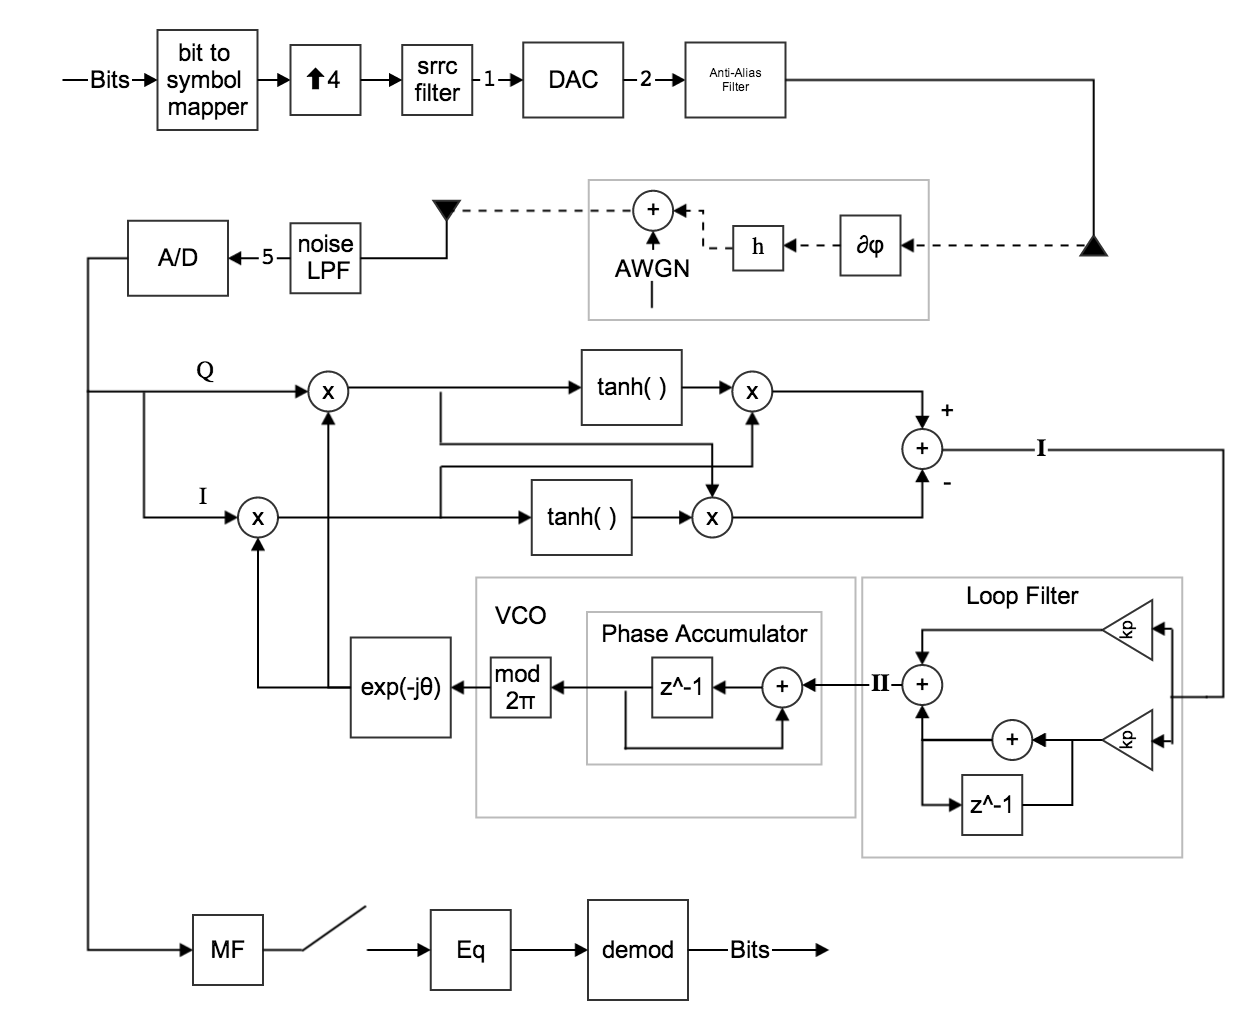
\includegraphics[width=\textwidth]{systemfinal.png}
\caption{Full System Block Diagram\label{fig:system}}
\end{figure}

Some vital information about the system parameters are listed below and each of the blocks seen on the figure are explained in detail in the following sections:
\begin{itemize}
\item Signal bandwidth = 10MHz
\item Square-root Raised Cosine Roll-off factor = 0.75
\item Channel Model = Bandlimited channel with AWGN and impulse response   $$h(t) = 0.1\delta(t + 100 \mathtt{ns}) + 0.8\delta(t -40 \mathtt{ns}) + 0.95\delta(t - 30 \mathtt{ns}) + 0.7\delta(t - 100 \mathtt{ns}) - 0.35\delta(t - 170 \mathtt{ns})  $$
\item Sampling Period = 0.1 ns
\item Equalizer Method: Zero Forcing
\item Number of taps = 2701
\item LPF Cut-off frequency = 5 MHz
\item Modulation scheme = QPSK/16QAM
\item Loop Filter coefficients =  0.05 and 0.001
\item Frequency offset = 5 kHz
\end{itemize}

\subsection{Bit Generation}
\label{sec:bits}
 To start with, a random bit generator output a stream of data (Appendix~\ref{app:random_bit_generator}). We used MATLAB psuedorandom generating functions to ensure the information would be as well distributed as possible. To further ensure the modeling was fair, the number of bits generated was set to 48000. 
\subsection{Modulation}
\label{sec:modulation}
The data stream was then passed into a bit-to-symbol mapper, transformed differently based on the modulation scheme  (Appendix~\ref{app:bittosym}).  Two modulation schemes were used as shown in Appendix~\ref{app:qpsk_mod},~\ref{app:qam_16_mod}.  These schemes were:
\begin{itemize}
\item Quadrature Phase Shift Keying [QPSK] which maps bits to symbols  as shown in the following constellation plot:

	\begin{figure}[H]
	\centering
	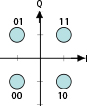
\includegraphics[width=.2\textwidth]{QPSK.jpg}
	\caption{QPSK constellation plot showing bit to 		symbol mapping}
	\end{figure}

\item 16 - Quadrature Amplitude Modulation [16-QAM] which maps bits to symbols as shown in the following constellation plot:

	\begin{figure}[H]
	\centering
	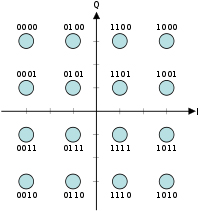
\includegraphics[width=.3\textwidth]	{16QAM.jpg}
	\caption{16-QAM constellation plot showing bit to 	symbol mapping}
	\end{figure}

\end{itemize}

It should be noted, both of the modulation schemes use Grey Coding.  Here, there is only one bit difference between neighboring symbols. This greatly decreases the bit error rate.

\subsection{Oversampling}
\label{sec:oversample}
In order to manipulate the signal without loss, the data was oversampled by four [Appendix~\ref{app:impulse_train}].  To do so, the code-block 'zero pads' the input so that an impulse train is passed along.  The sampling rate, because of this, exceeded the Nyquist sampling rule but allowed us to have some extra leeway for processing.   

\subsection{Pulse Shaping}
\label{sec:srrc}
To approximate a real system, the signal is put through a square root raised cosine filter in order to represent symbols as pulses that can be transferred over a channel. This filter has the following impulse response:

 \[
 h(t) = \begin{dcases*}
        1-\beta+4\frac{\beta}{\pi} &  $t = 0$\\ \\        
        \frac{\beta}{\sqrt{2}}\left[\left(1+\frac{2}{\pi}\right)\sin\left(\frac{\pi}{4\beta}\right)+\left(1-\frac{2}{\pi}\right)\cos\left(\frac{\pi}{4\beta}\right)\right] & $t=\pm \frac{T_s}{4\beta}$ \\ \\
        \frac{\sin\left[\pi\frac{t}{Ts}\left(1-\beta\right)\right]+4\beta\frac{t}{Ts}\cos\left[\pi\frac{t}{Ts}\left(1+\beta\right)\right]}{\pi\frac{t}{Ts}\left[1-\left(4\beta\frac{t}{Ts}\right)^2\right]} & $otherwise$ \\
        \end{dcases*}
\]

as implemented in Appendix~\ref{app:sqrt_raised_cosine}.  \\

One can question why another pulse shape, such rectangular function, isn't used in the project. The square root raised cosine pulse is a common and effective tool to combat inter symbol interference [Section~\ref{sec:ISIbackground}].  This interference is caused by the fact that it is a Nyquist pulse with a flat spectrum.  In other words, because the raised cosine has zero impulse response at all integer multiples of its period, correct sampling can perfectly reconstruct the signal without having delayed symbols muddle the waveform. 

\subsection{Digital-to-Analog Conversion}
\label{sec:da}
The output of this shaping filter (\#1 in Figure~\ref{fig:system}) is fed into a Digital-to-Analog Converter (DAC).  A DAC takes the digital samples and zero-order holds them at a constant voltage, creating an analog signal. At this point, the signal is assumed to be sent through physical components. The demonstration of this conversion can be seen in Figure~\ref{fig:dtoa} \\

The implementation of this block can is shown in Appendix~\ref{app:da}..

\subsection{Anti-Aliasing Reconstruction Filter}
\label{sec:reconstruction}
After the analog to digital conversion, a reconstruction filter (also called an anti-aliasing filter) bandlimits the analog waveform output from the DAC (\#2 in Figure~\ref{fig:system}).  The high frequency content contained in the stair-case digital signal is undesirable since it can create aliasing of wrongfully high frequency waves. To avoid this, the Low Pass Filter is used for the reconstruction.  Ours is modeled as a Butterworth filter, or a maximally flat magnitude filter.  The aim of the filter is to have uniformly flat passband frequency response and roll to zero in the stopband.  As with all filters, the cutoff frequency parameter sets the bands and the order of the filter determines the roll-off of the frequency response in the stopband.  We used a fourth order Butterworth so that the roll-off was $80 \mathtt{\frac{dB}{dec}}$.  We set the cutoff frequency approx. to 5 $\mathtt{kHz}$ at the TX part. The interior workings of the filter are not pertinent to this project, so the code in Appendix~\ref{app:butterworth} uses built-in MATLAB functions. Furthermore the issues and challenges caused by bilinear transformation of an analog filter to digital filter and TX cut-off frequency sensitivity are addressed in Section~\ref{sec:issues}. \\

At this point (\#3 in Figure~\ref{fig:system}), the waveform is ready to be transmitted through the medium.\\

A demonstration of the output of this filter can be seen in Figure~\ref{fig:dtoa}.

\begin{figure}[H]
\centering
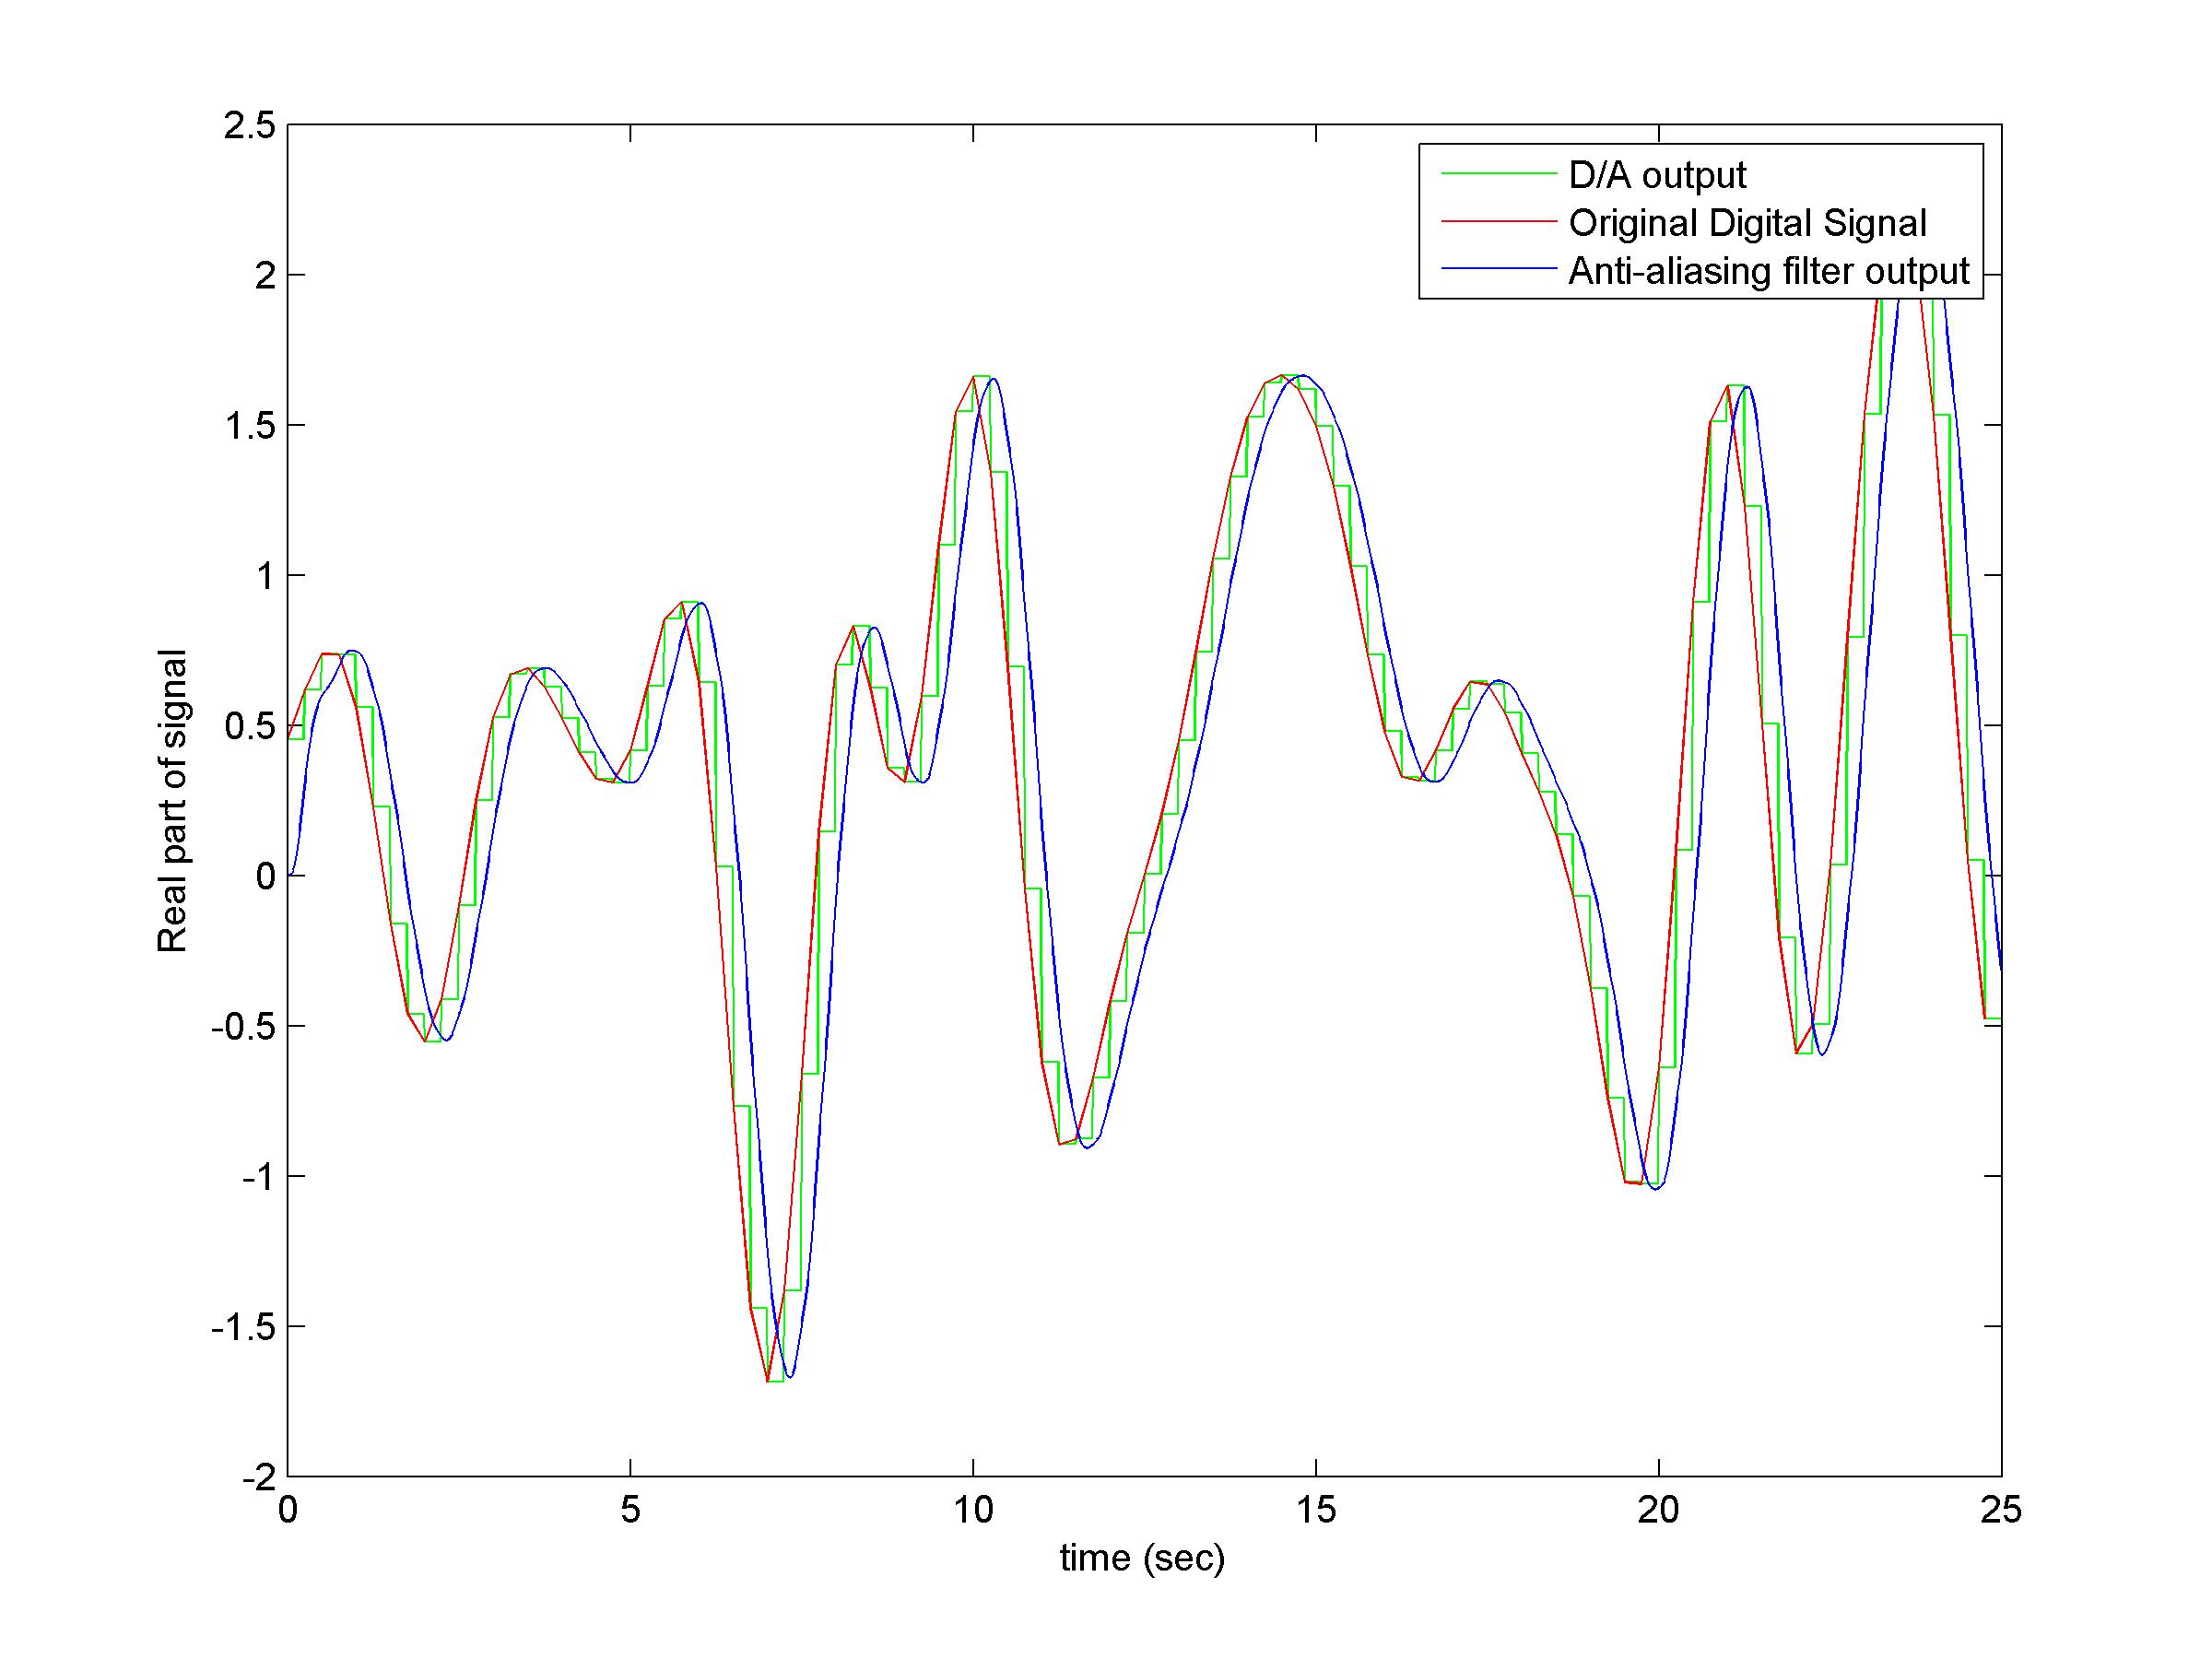
\includegraphics[width=\textwidth]{DtoA.jpg}
\caption{The original digital signal and the outputs of D/A converter and anti-aliasing filter at SNR=100dB for the first 100 symbols (QPSK modulation)\label{fig:dtoa}}
\end{figure}

\subsection{Channel Medium}
\label{sec:channel}
After processing the data at the TX end of the system, it is sent through a bandlimited channel which is modeled to produce a phase error and have additive white Gaussian noise. 

\subsubsection{Phase Error}
\label{sec:phaseError}
To enhance the realism of the model, non-coherent error was included in the transmission. The $\delta\phi$ block represents a frequency offset on the carrier.  The effect of this is to blur the symbol constellations.  The new block was modeled by introducing a first order phase term.  Recall, phase is related to frequency by Equation~\ref{eq:phaseToFreq}.

\begin{equation}
\label{eq:phaseToFreq}
f(t) = \frac{1}{2 \pi} \phi^\prime(t)
\end{equation}

Appendix~\ref{app:freq} shows how this was implemented in the simulations.  We used a frequency offset of $100 \mathtt{kHz}$.  

\subsubsection{Channel Gain}
\label{sec:channelFilter}
We have the following bandlimited channel response installed in our system model:
 $$h(t) = 0.1\delta(t + 100 \mathtt{ns}) + 0.8\delta(t -40 \mathtt{ns}) + 0.95\delta(t - 30 \mathtt{ns}) + 0.7\delta(t - 100 \mathtt{ns}) - 0.35\delta(t - 170 \mathtt{ns})  $$
 
This has to be converted into vector form in order to process in MATLAB. Thus the following calculation is made: 
 
 $$h(t) = 0.1\delta(t + 100 \frac{\mathtt{ns}}{T_s}) + 0.8\delta(t -40 \frac{\mathtt{ns}}{T_s}) + 0.95\delta(t - 30 \frac{\mathtt{ns}}{T_s}) + 0.7\delta(t - 100 \frac{\mathtt{ns}}{T_s}) - 0.35\delta(t - 170 \frac{\mathtt{ns}}{T_s})  $$
 
 $$ \Rightarrow h[k] = 0.1\delta(k + 1000) + 0.8\delta(k -400 T_s) + 0.95\delta(k - 300) + 0.7\delta(k - 1000) - 0.35\delta(k - 1700)$$
 
Although this channel introduces significant ISI, we have perfect knowledge of the channel, so handling the interference is not difficult. \\

The implementation of the bandlimited channel is shown in Appendix~\ref{app:bandlimited} and~\ref{app:chan_snip}.

\subsubsection{Noise}
\label{sec:awgn}
The channel additionally has a source of Additive White Gaussian Noise (AWGN) as implemented in Appendix~\ref{app:awgn_channel}. The variance of this channel noise is determined by the SNR values picked at the beginning of each simulation. We can relate the two by the following:

$$\sigma^2 = \frac{S}{10^{SNR/10}}$$
where S is the average signal power of the chosen modulation scheme.  The AWGN concludes the channel model (\#4 in Figure~\ref{fig:system}). \footnote{We could have made this noise be colored by the channel itself: move the summer before the channel block.  However, we then could easily introduce a whitening filter to flatten the frequency response back to Gaussian.  Such a complication could be added in future models.} 

\subsection{Noise Limiting Filter}
\label{sec:noiseLPF}
Prior to digitization, an anti-aliasing low-pass filter constrains, or bandlimits, the channel-filtered waveform (\#5 in Figure~\ref{fig:system}).  In this setting, the LPF protects against aliasing of high frequency content being recorded at the lower frequency.  We use the same Butterworth filter (implemented in Appendix~\ref{app:butterworth}) and set the cut-off frequency to approximately 5 $\mathtt{kHz}$ at the receiver. The output of this filter is demonstrated in Figure~\ref{fig:atod}. Again, issues and challenges caused by bilinear transformation of an analog filter to digital filter and RX cut-off frequency sensitivity are addressed in Section~\ref{sec:issues}.

\subsection{Analog-To-Digital Converter}
\label{sec:adc}
To bring the analog waveform back to the digital world, an Analog-to-Digital converter is used with the implementation shown in Appendix~\ref{app:ad}.  From here (\#6 in Figure~\ref{fig:system}) on out, the waveform is back in the digital domain for processing. \\

The output of this block can be seen in Figure~\ref{fig:atod}.  Issues and challenges caused by the converter sampling instances are addressed in Section~\ref{sec:issues}.

\begin{figure}[H]
\centering
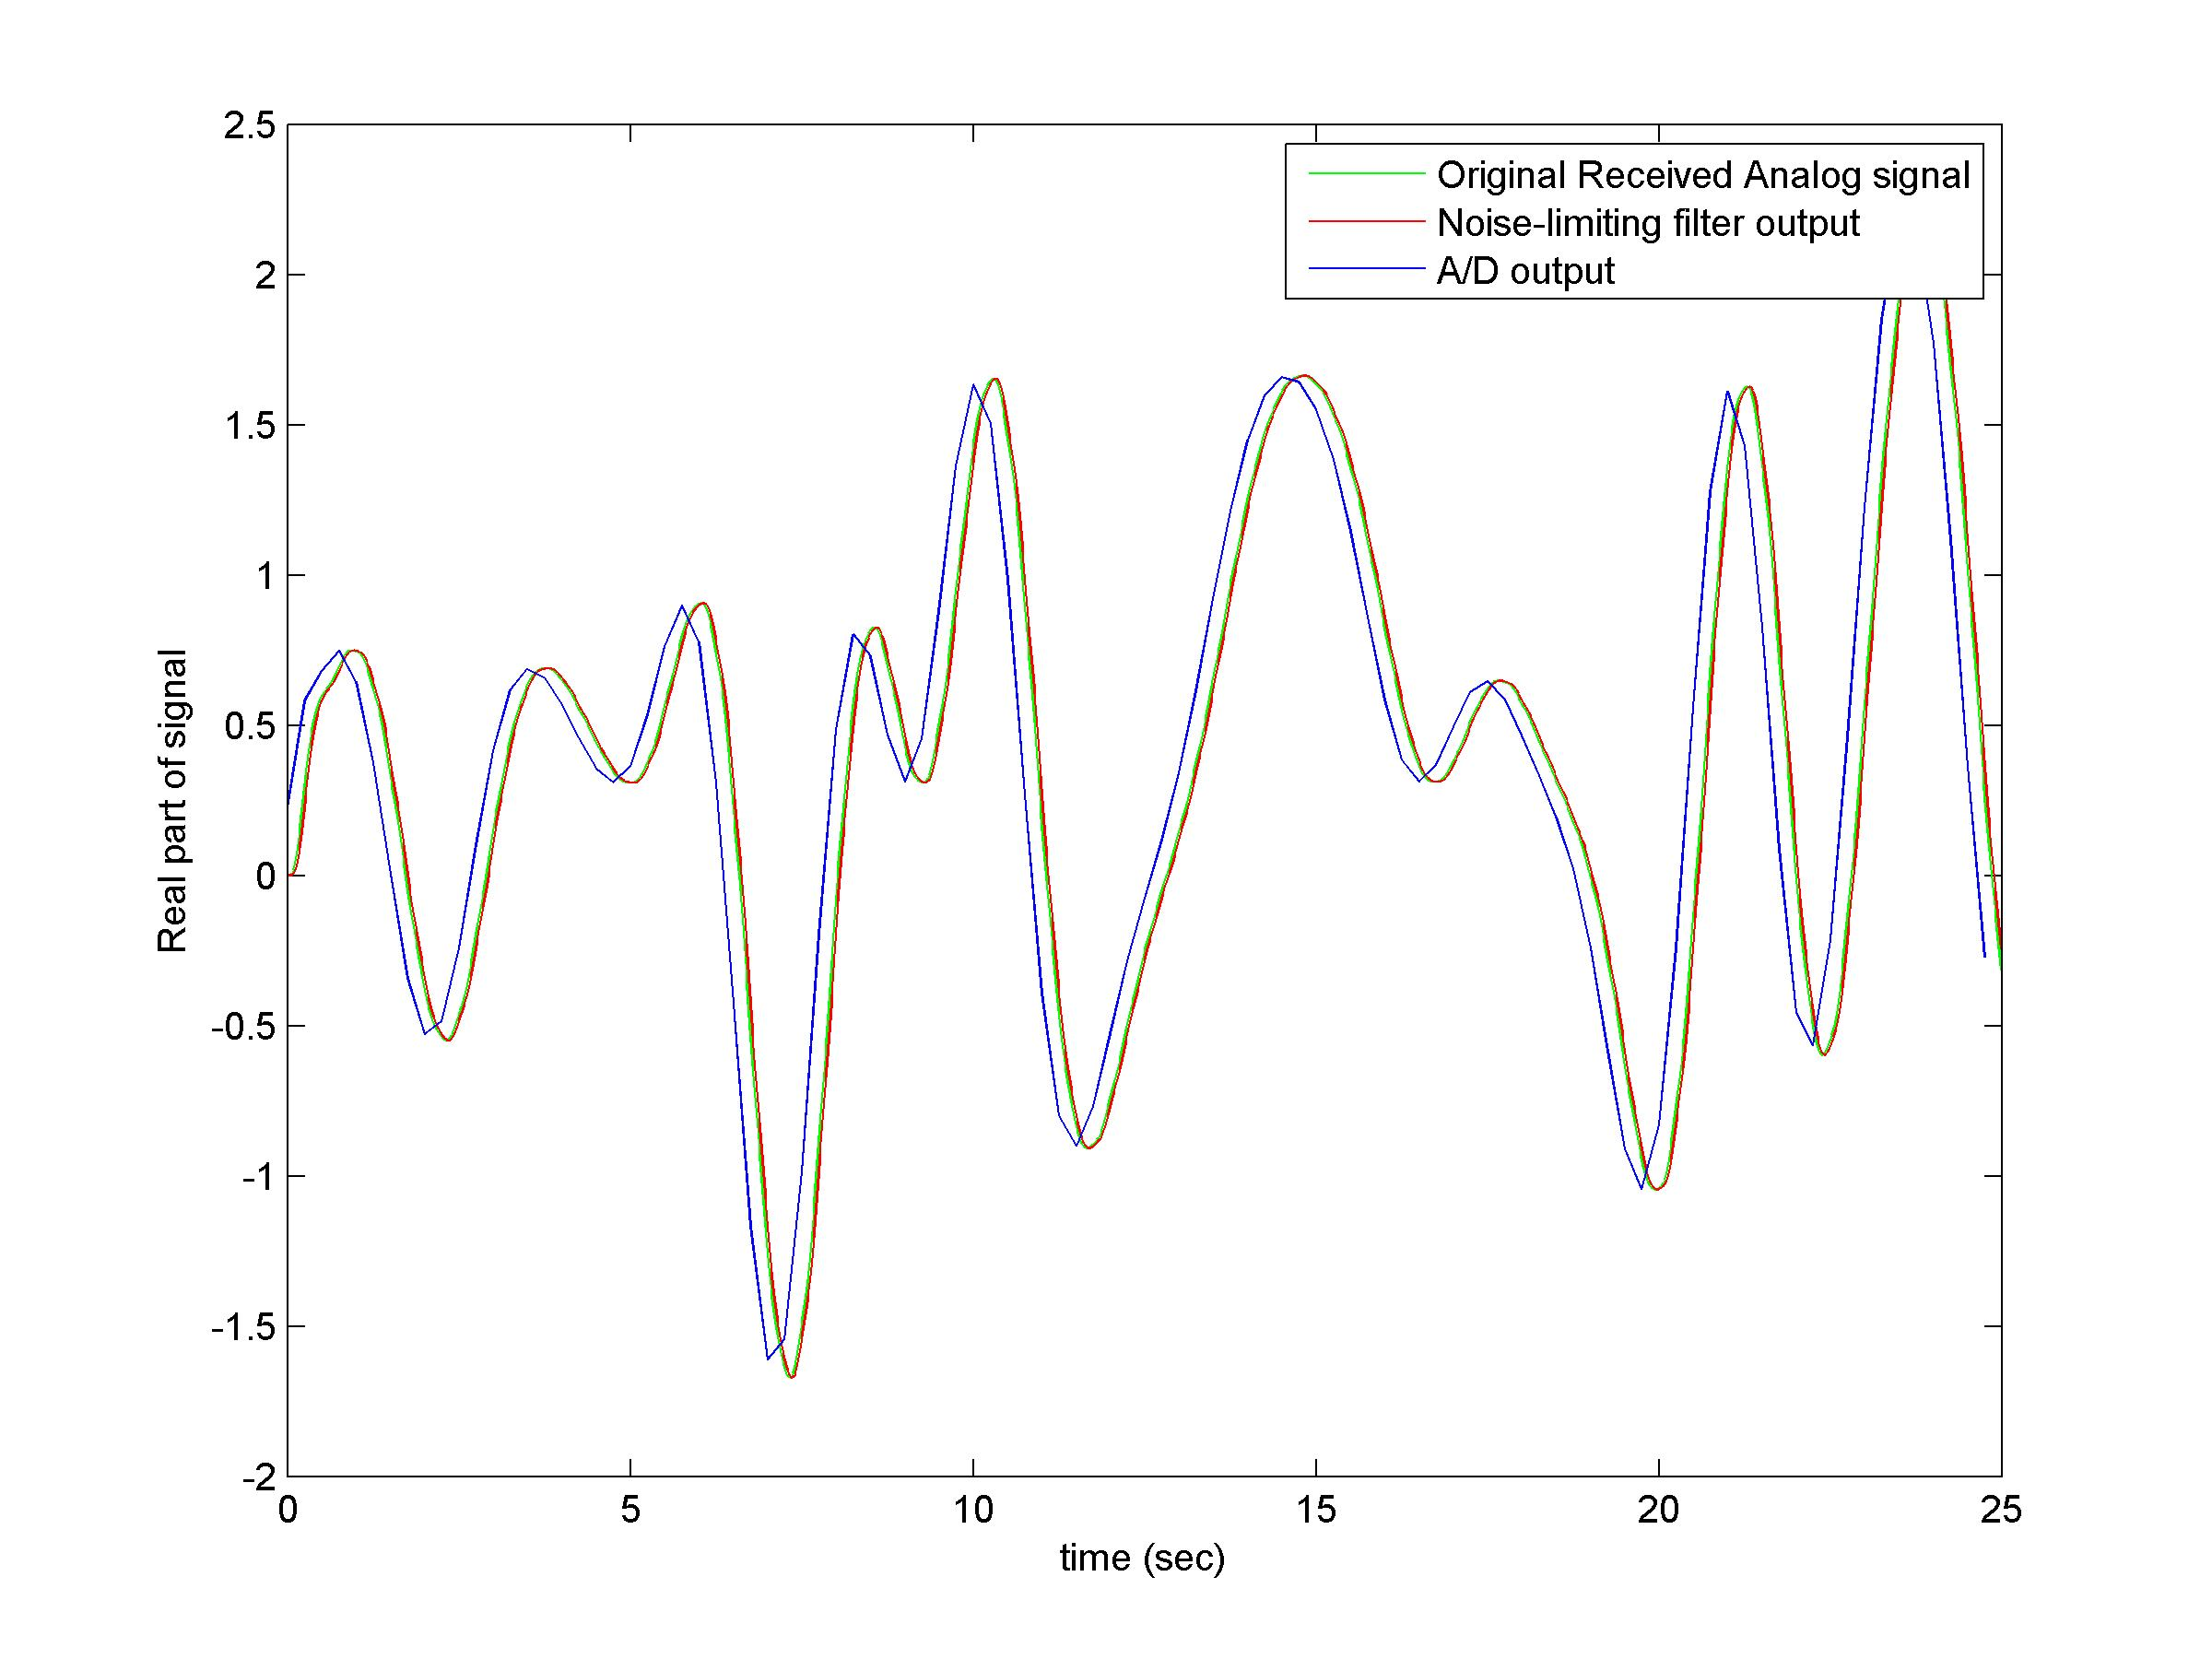
\includegraphics[width=\textwidth]	{AtoD.jpg}
\caption{The original received analog signal and the outputs of A/D converter and noise-limiting filter at SNR=100dB for the first 100 symbols (QPSK modulation)\label{fig:atod}}
\end{figure}

\subsection{Tracking Loop}
\label{sec:tracking}
The frequency offset recovery is accomplished via a Costas Loop whose implementation is given in Appendix~\ref{app:RX_snip}. The I and Q component of the received signal (\#7i and \#7q in Figure~\ref{fig:system}) are both sent through a $\tanh\left(\cdot\right)$ block in order to discern their sign.  This works because, for $k>>1$, $\text{sign}\left(x\right) \approx \tanh \left(x\right)$.  These $\pm1$ signals are multiplied by the opposite component signal.  The I component is then subtracted from the Q component, creating a phase error metric [Equation~\ref{eq:costas}].  The phase error is labeled in Figure~\ref{fig:system} as \#8. 

\begin{align}
  \label{eq:costas}
  S_{\rom{1}} &= \left[I\left(t\right)\sin\left(\phi_e\right)+Q\left(t\right)\cos\left(\phi_e\right)\right]\text{sign}\left(I\left(t\right)\cos\left(\phi_e\right)- Q\left(t\right)\sin\left(\phi_e\right)\right)\nonumber \\
  &\qquad {} - \left[I\left(t\right)\cos\left(\phi_e\right)-Q\left(t\right)\sin\left(\phi_e\right)\right]\text{sign}\left(I\left(t\right)\sin\left(\phi_e\right)+Q\left(t\right)\cos\left(\phi_e\right)\right)
  \end{align}

The error is run into the loop filter, the first integrator in the feedback leg of the loop.  Further background on feedback loops is given in detail in Section~\ref{sec:feedback}. The output of the loop filter is sent into another integrator, a Voltage Controlled Oscillator (VCO). \\

A VCO is a device whose output oscillation is variably controlled by the voltage level of the input.  The transfer function, relating the input to the output, for this block is shown in Equation~\ref{eq:vco}. The integral action can help eliminate phase error. To implement a VCO in simulation, a phase accumulator does the integration action and then, to keep the result in the correct domain, the result is put through a modulo $2\pi$ block. \\

\begin{align}
\label{eq:vco}
\phi_{\text{out}} &= \int \! k_{VCO}V_{in} \mathrm{d}t
\end{align}

Finally, after the VCO and feedback action, the I and Q components are recombined by a summer (\#10 in Figure~\ref{fig:system}). \\

The crucial point in designing the feedback loop is finding the right coefficients for the loop filter.  The filter must provide a fast tracking of the frequency offset. Doing so ensures the loop reaches the steady state as fast as possible, allowing for fewer errors in the output bits. \\

Another important issue we had to address is the challenges caused by using a phase tracker and two integrators to cancel out the frequency offset. This is discussed in Section~\ref{sec:issues}.

\subsection{Matched Filter}
\label{sec:matched}
After the signal is back to a complex form, a matched filter is used for optimal detection. The same square root raised cosine pulse (as implemented in Appendix~\ref{app:sqrt_raised_cosine}) is used to pick up the waveform (\#11 in Figure~\ref{fig:system}).

\subsection{Sampler}
\label{sec:sample}
After the matched filter, the signal has to be sampled at 10 $\mathtt{GHz}$.  We should keep in mind that the signal is oversampled by a factor of four in the TX end of the system. In other words the sampler has to pick one of the four oversampled points.  We would prefer the sampler pick the point with the highest value - this would mean it matched the best point. Usually this is the value at the integer multiples of  $T_s$. \\

The implementation of this block is shown in Appendix~\ref{app:sampler}.

\subsection{ZF Equalizer}
\label{sec:equal}
Because of Inter-Symbol Interference (ISI), there is an equalizer set to level the system frequency response.  Section~\ref{sec:ISIbackground} further explains ISI and equalization.

The equalizer implemented here is a Zero-Forcing (ZF) architecture, as shown in~\ref{app:RX_snip} and~\ref{app:zf}. To satisfy the Zero ISI Condition~\ref{thm:zero}, the weight vector, $\mathbf{f}$, must perfectly negate all taps except the present-time one.  The present received symbol is a column within the $R$ matrix: $\mathbf{r}[i]$, often chosen to be the center one.  
$$ \mathbf{f}^{\ast}R = \mathbf{w}[i]^{\top} $$
Here, we used  $\mathbf{w} [i] \in \mathbb{R}^n$ to represent the i$^{th}$ Standard basis vector, or a column of zeros except in row $i$.  In this setting, we can find the tap weight vector to accomplish this by Equation~\ref{eq:zf}. 

\begin{equation}
\label{eq:zf} 
\mathbf{f}_{ZF} = R \left(R^{\ast}R \right)^{-1} \mathbf{w}
\end{equation}

\subsection{Demodulation}
\label{sec:demod}
After the equalization (\#11 in Figure~\ref{fig:system}), the signal is ready to be mapped back into bits.  The demodulation in this block is the reverse of mapper used in the transmitter.  The implementation of this is shown in Appendix~\ref{app:16qam_demod}.  \\

At this step, we are finally ready to evaluate how well the system worked.

\section{Issues and Challenges}
\label{sec:issues}
\subsection{Bilinear Transformation}
An important issue we had to deal with was the bilinear transform MATLAB uses to transform the analog Butterworth filter into the discrete domain.  As shown in the figure below, the $tan(.)$ function is nonlinear at higher frequencies and linear at frequencies close to zero:

\begin{figure}[H]
\centering
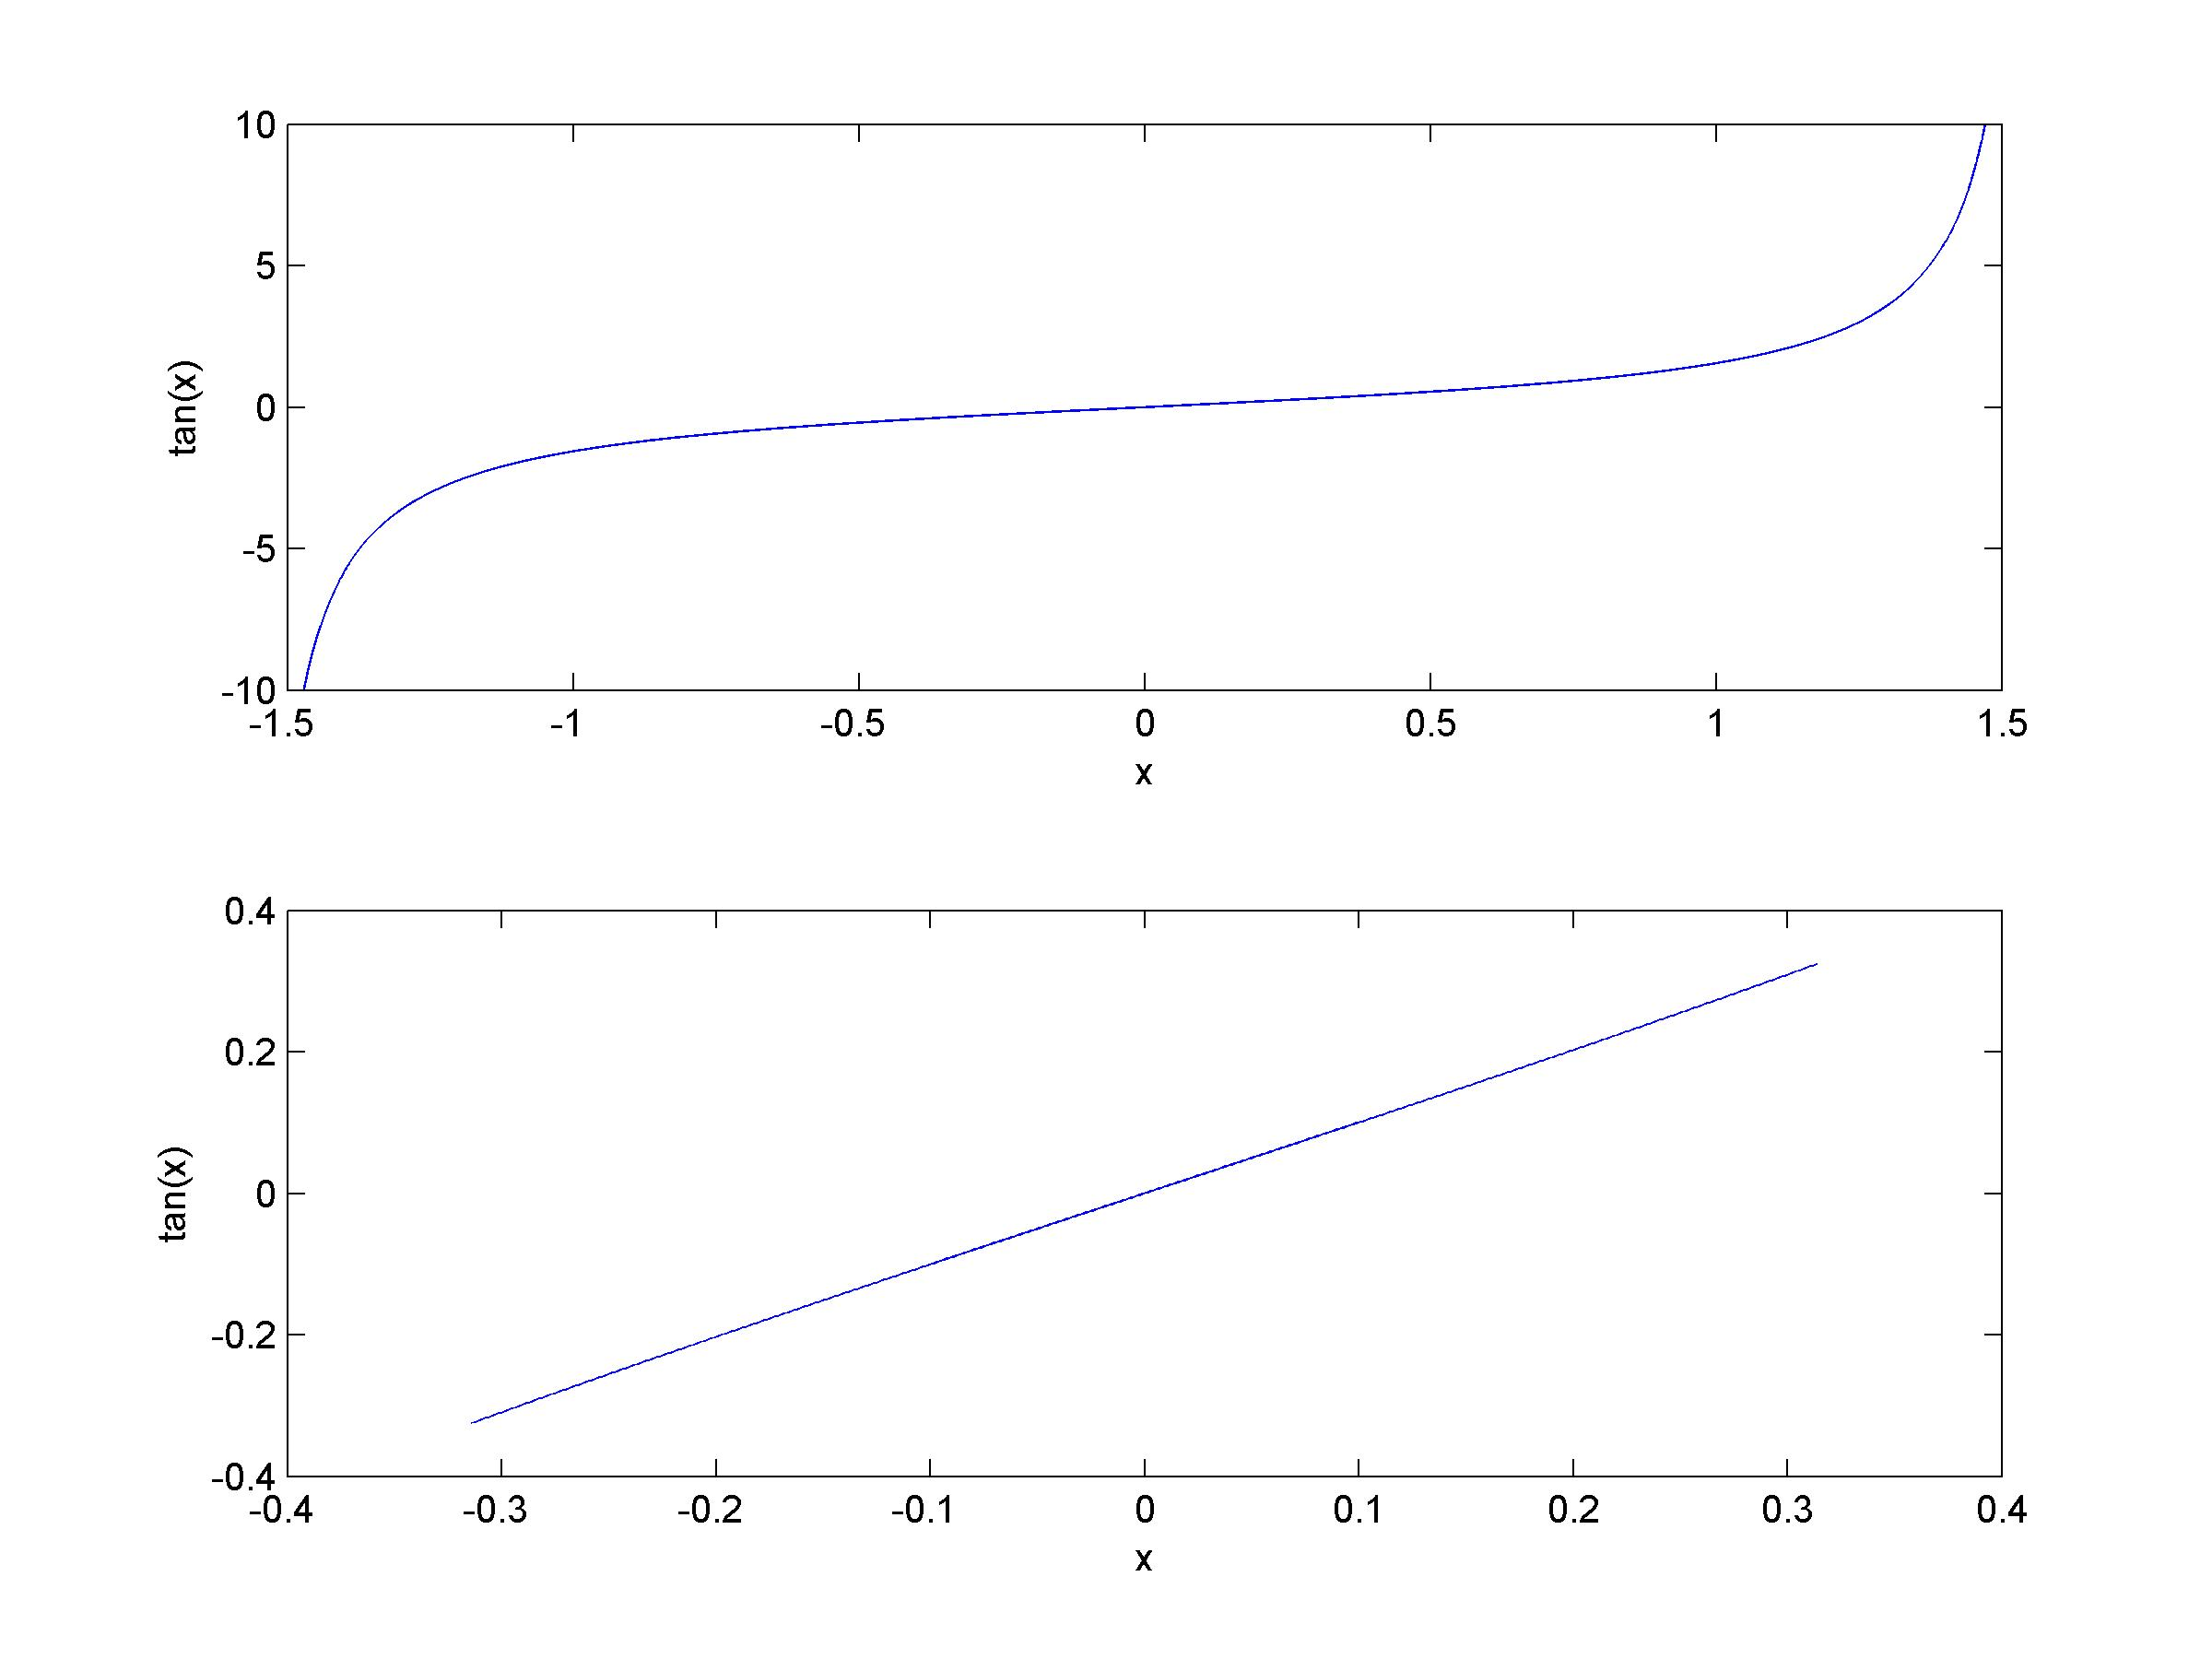
\includegraphics[width=0.7\textwidth]{tan_graph.jpg}
\caption{SER plot as a function of delay at the samplin g points of the A/D converter at SNR=20dB (QPSK modulation). \label{fig:delay}}
\end{figure} 

Thus, in order to have normalized cut-off frequencies at the linear regions (assumed to be linear around $\left[ -\pi/10,\pi/10 \right] $) of the $tan(.)$ function, the over sampling rate of the analog signal is set to 80 times more than the digital signal. \\

\subsection{TX Cut-off Frequency Sensitivity}
\label{sec:TXcutoff}
A sensitivity analysis is done for the cutoff frequency of the TX reconstruction filter. Recall, this filter is in place to bandlimit the DAC output so the high frequency content in the `stairs' does not create aliases in the lower passband. The filter model is controlled by a normalized cutoff frequency, where zero and one are mapped to $\left(0,f_s\right)$.  As such, we expect that the cutoff frequency will not make much difference except if it is lower than $\pi/$(over sampling size of analog signal).  Even by choosing $f_c$ near $\pi/10$, the end of assumed linear region, all frequencies above the sampling frequency will be attenuated and the filter serves its purpose.  However, if $f_c$ gets too low, the information in the waveform may be lost. Figure~\ref{fig:freqTX} shows the sensitivity analysis of the anti-aliasing LPF normalized cutoff frequency. The graph confirms the expected behavior discussed above.

\begin{figure}[H]
\centering
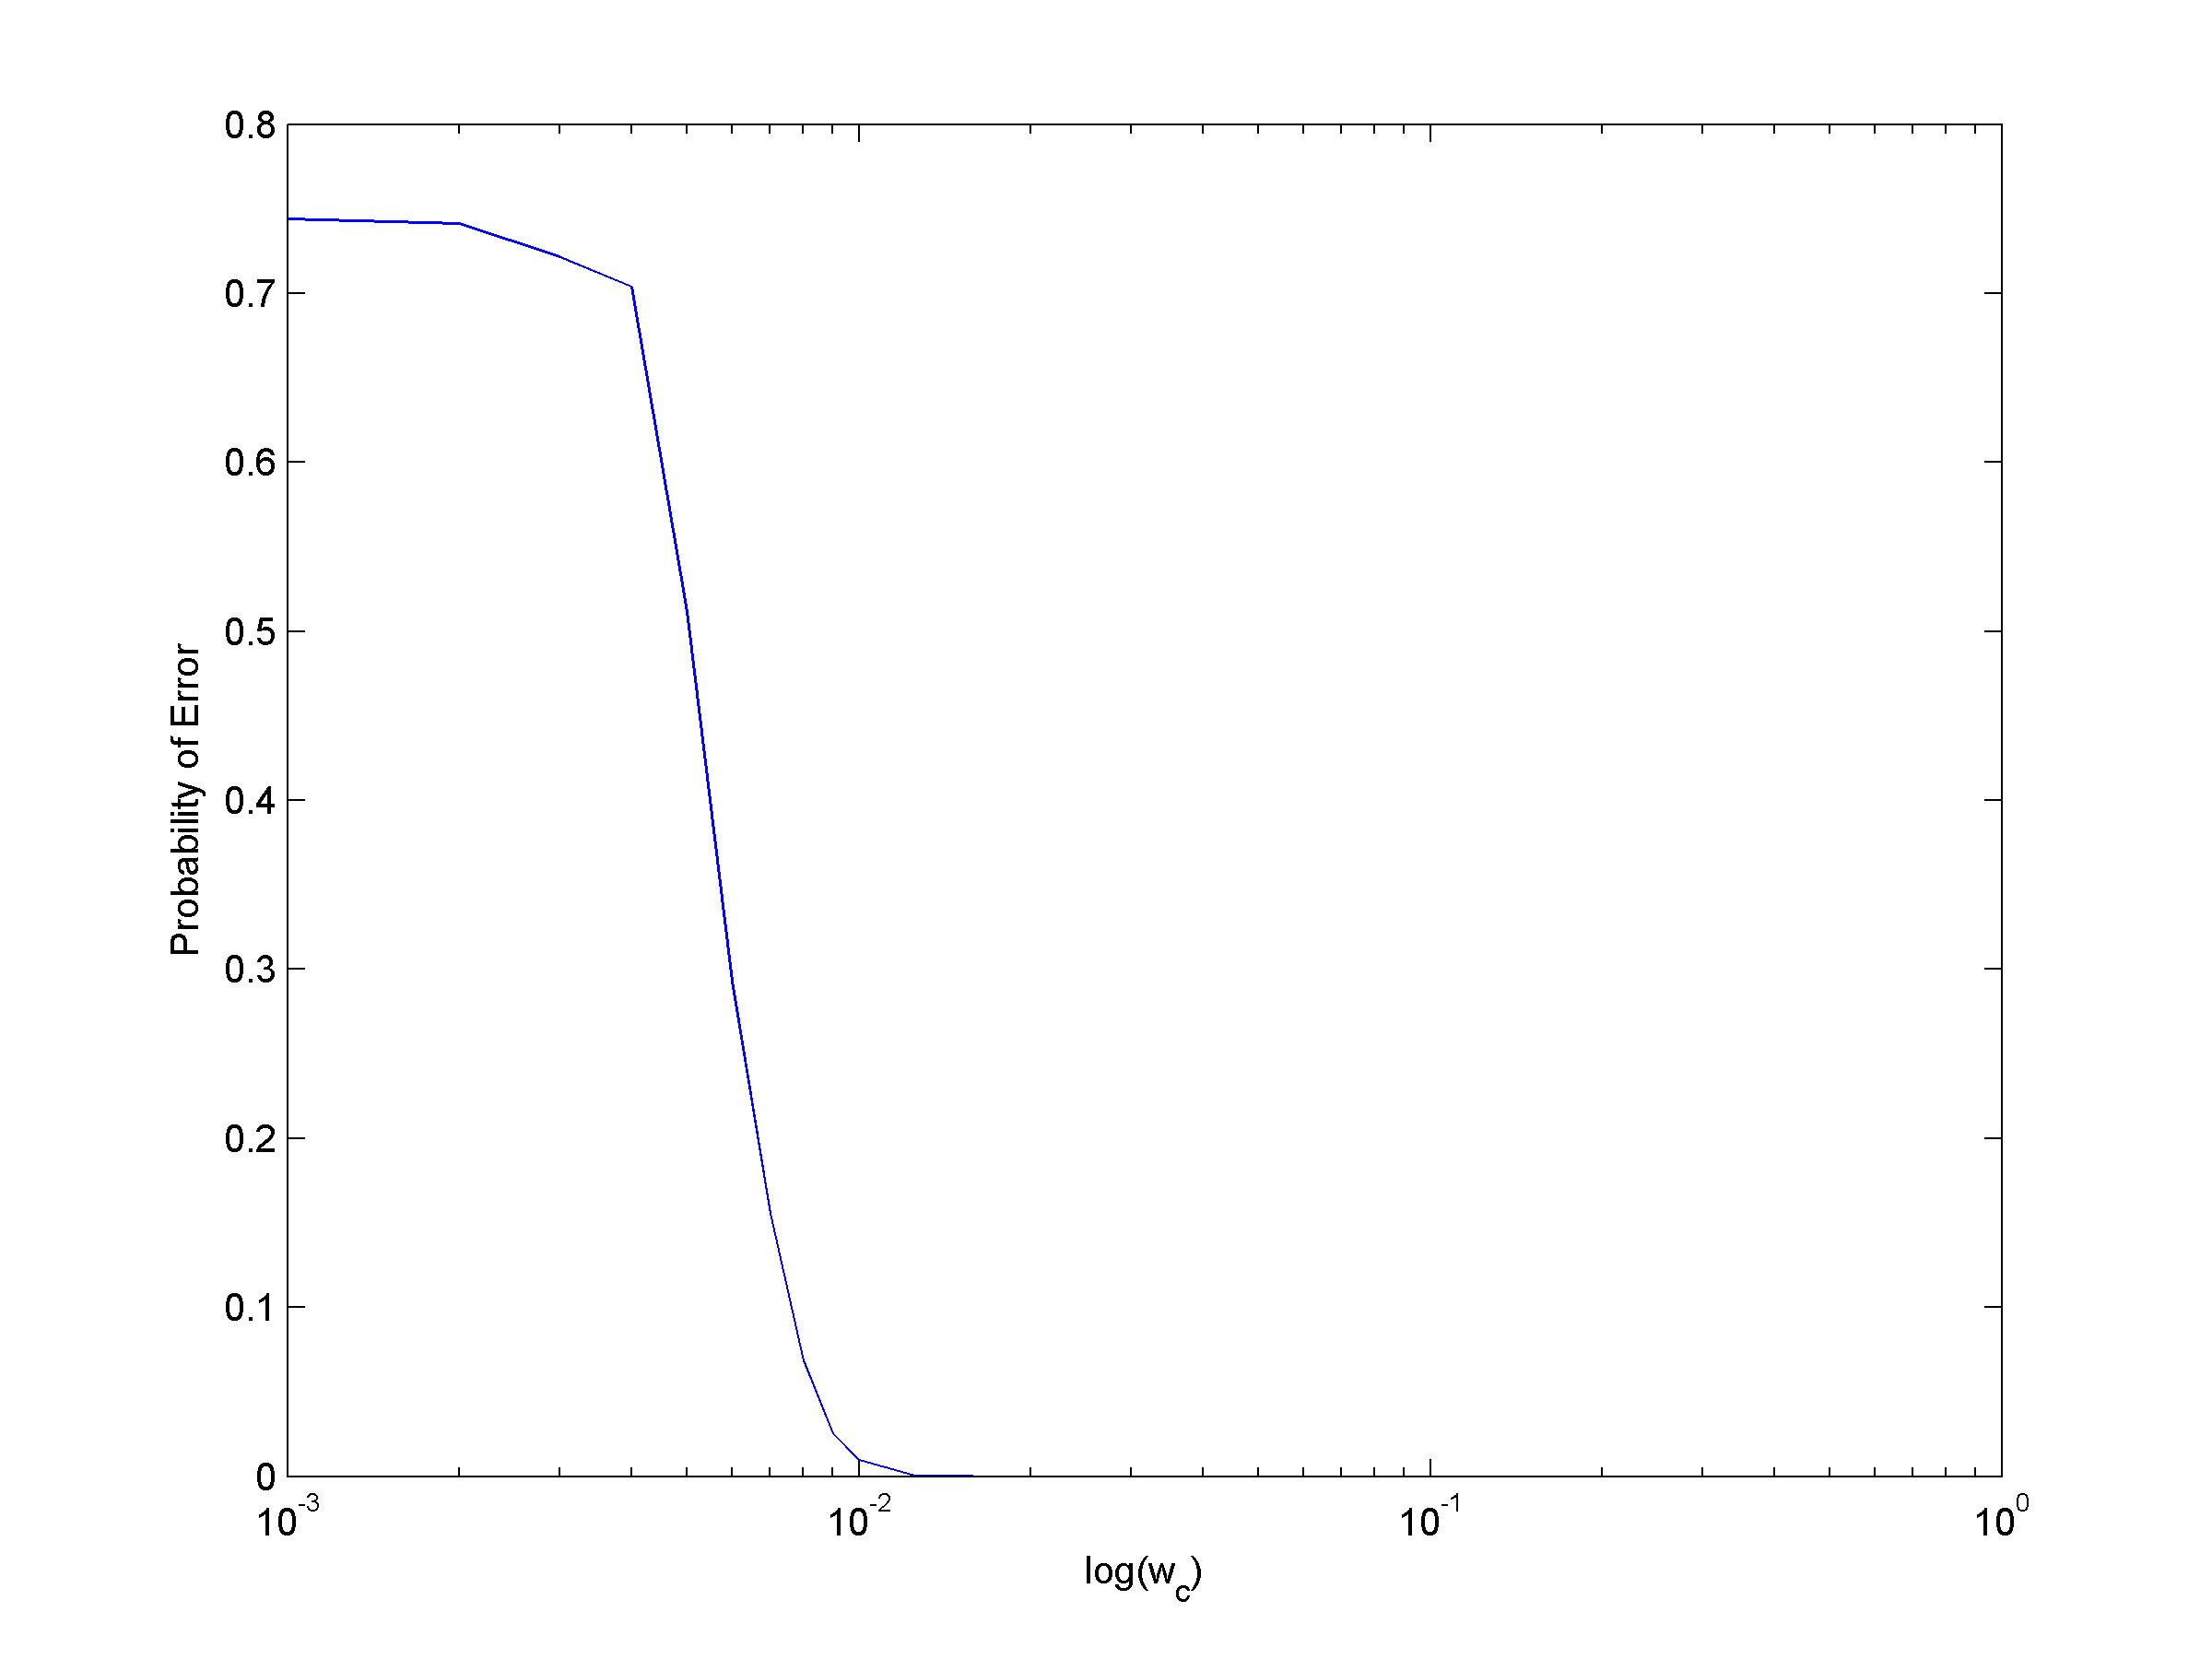
\includegraphics[width=0.6\textwidth]{freqTX.jpg}
\caption{SER plot as a function of cutoff frequency in the TX anti-aliasing Reconstruction filter at SNR=20dB (QPSK modulation). \label{fig:freqTX}}
\end{figure}

\subsection{RX Cut-off Frequency Sensitivity}
\label{sec:RXcutoff}
We also performed a sensitivity analysis on the cutoff frequency in the RX noise-limiting filter. This filter was aimed to low pass filter the high frequency content from the noise and only allow the signal through. The same filter model was used with a lower cut-off frequency, so a similar trend was expected. Again at near zero cutoff,  we expect loss of data. But this time, when the cut-off frequency is increased to the limits of the linear region, we see an increase of the Bit Error Rate due to the fact that more noise is passing through the filter. Figure~\ref{fig:freqRX} shows the sensitivity analysis of the noise-limiting LPF normalized cutoff frequency. 

\begin{figure}[H]
\centering
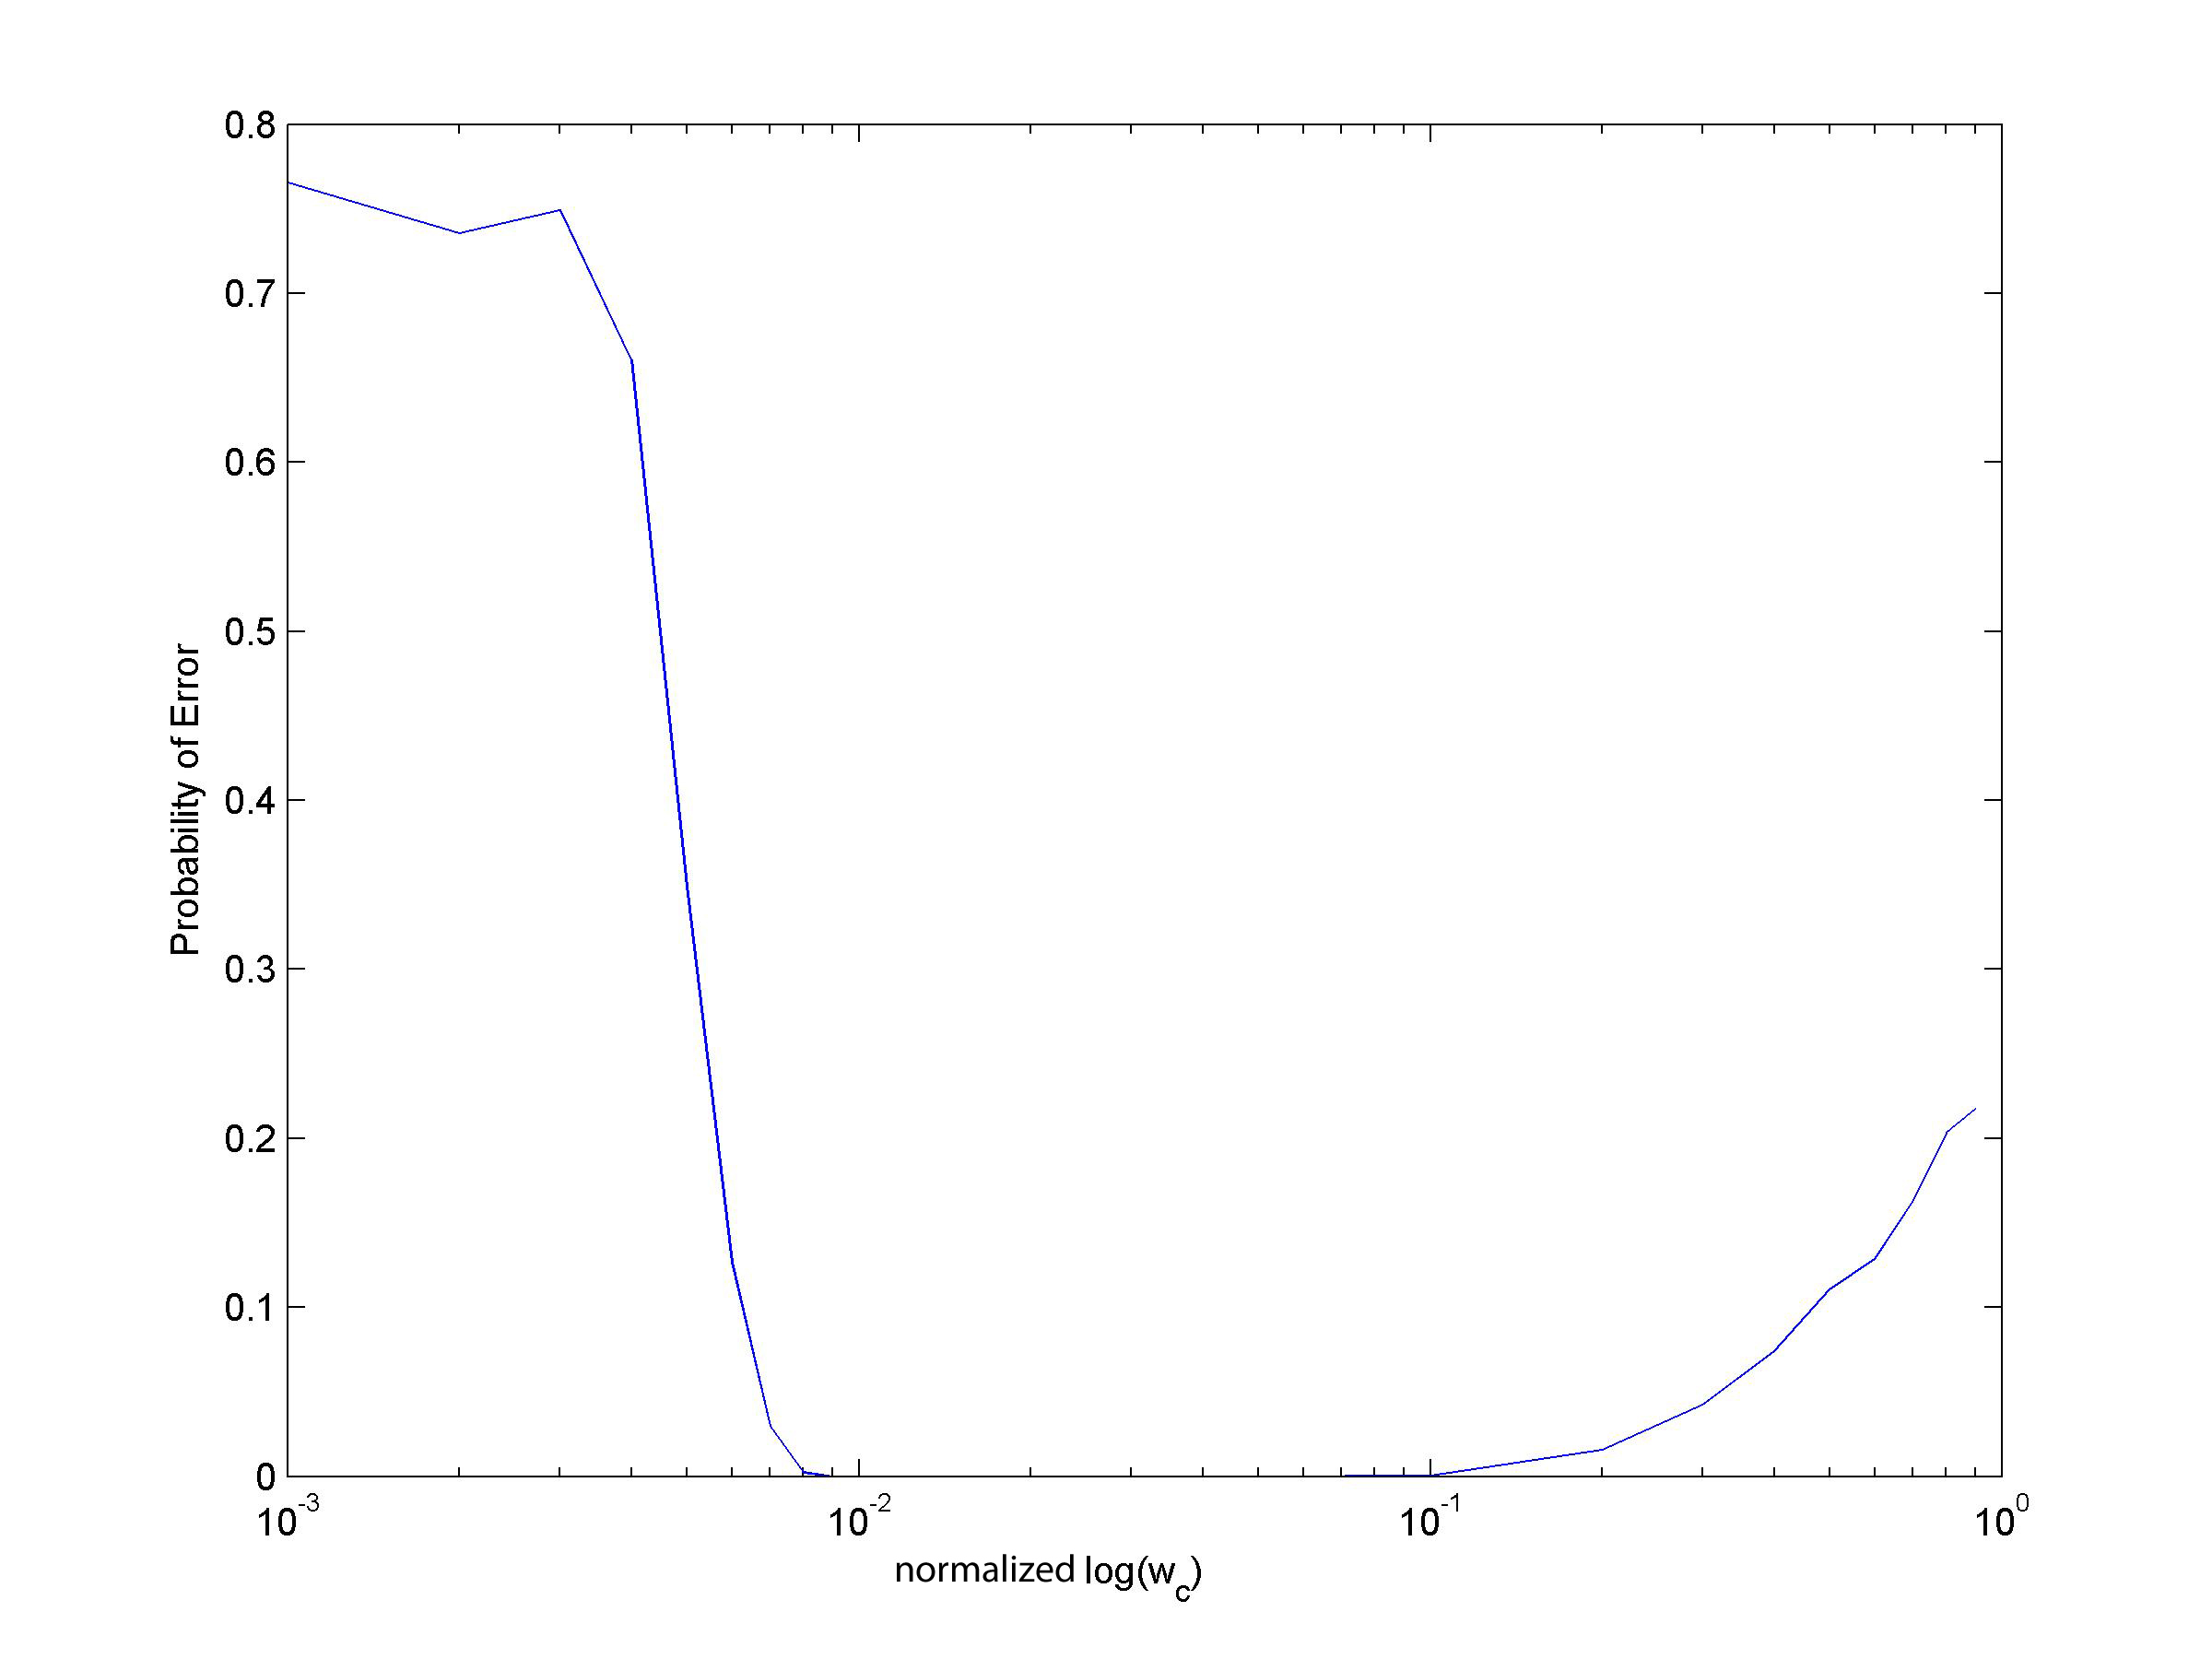
\includegraphics[width=0.6\textwidth]{freqRX.jpg}
\caption{SER plot as a function of cutoff frequency in the RX noise-limiting filter at SNR=20dB (QPSK modulation). \label{fig:freqRX}}
\end{figure}

\subsection{Sampling Delay Sensitivity}
\label{sec:delaySensitivity}
The importance of sampling timing on the bit error rate is crucial due to the fact that we use low pass filters at both RX and TX.  These filters delay the signals passing through them and may through off the sampling timing. By doing a sensitivity analysis of the delay through the system, we found the A/D will sample at varying degrees of synch.  As seen in Appendix~\ref{app:delay}, when all other parameters (SNR and cutoff frequencies, etc.) are kept at their optimal, we find the system works best at sampling delays of one and two. This is shown in Figure~\ref{fig:delay}.

\begin{figure}[H]
\centering
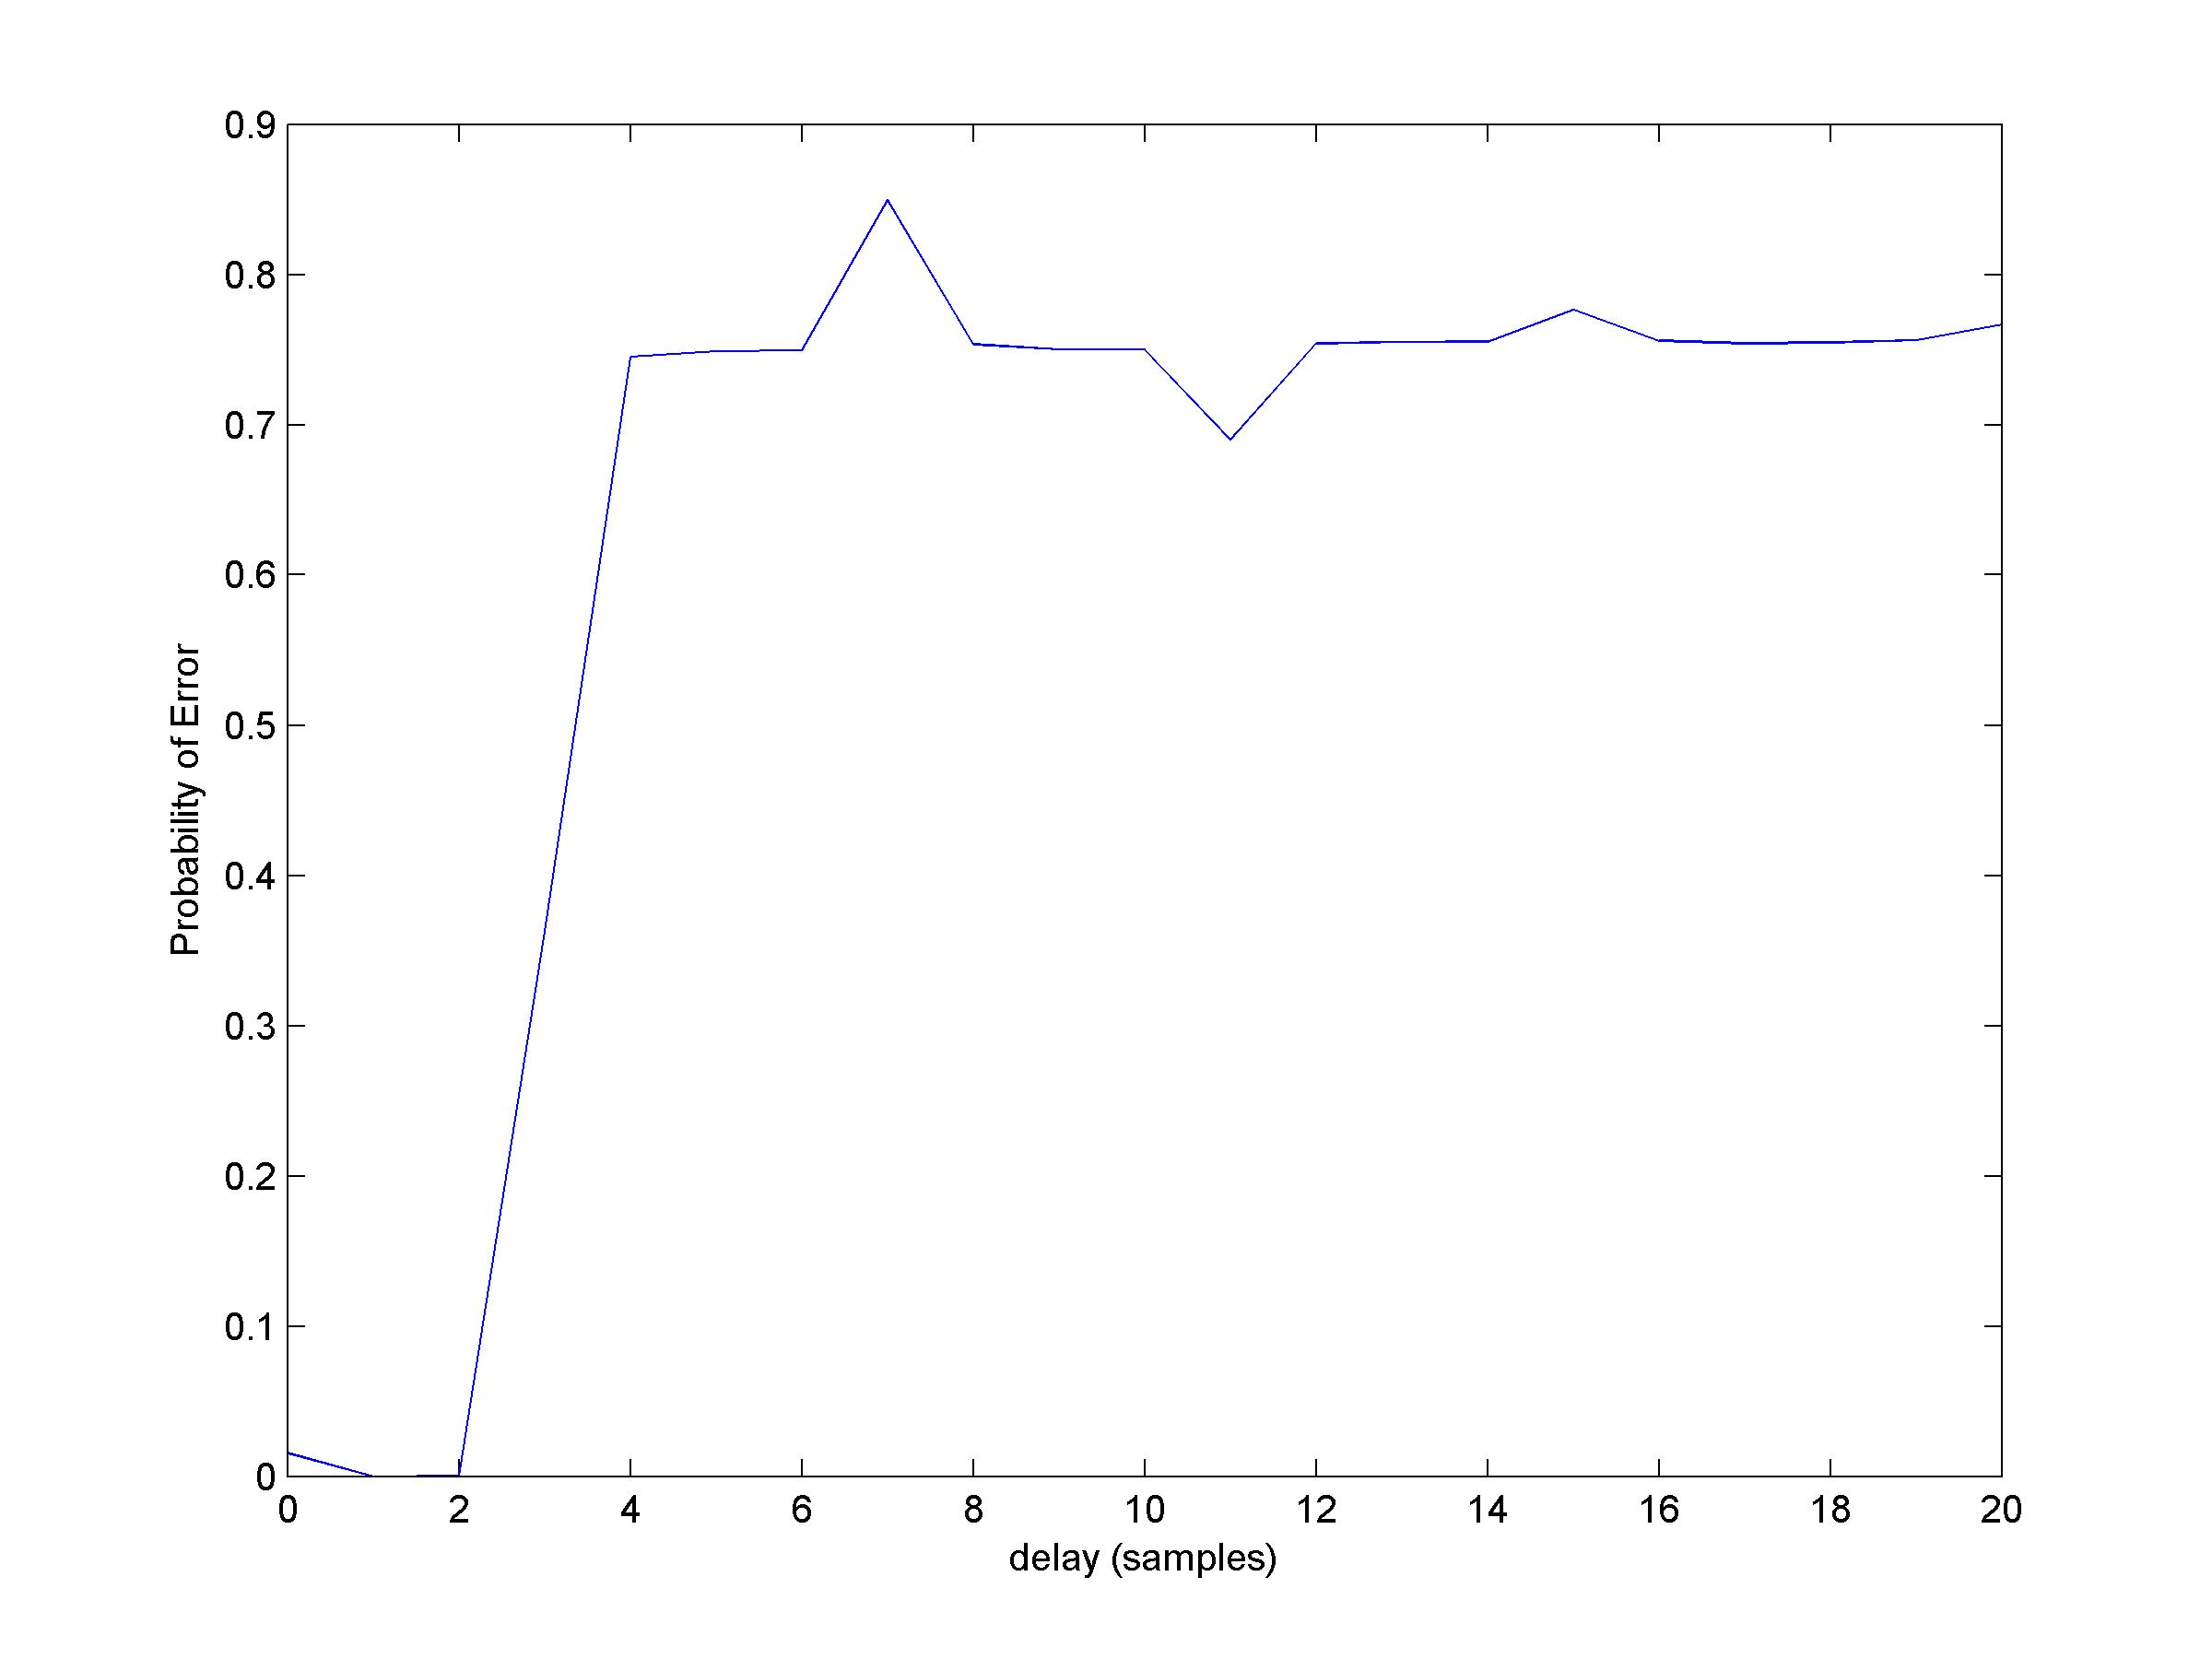
\includegraphics[width=0.6\textwidth]{delaySensitivity.jpg}
\caption{SER plot as a function of delay at the samplin g points of the A/D converter at SNR=20dB (QPSK modulation). \label{fig:delay}}
\end{figure}

\subsection{ZF Equalizer Noise-Enhancement}
\label{sec:noiseEnhancement}
A common metric for the cost of using Zero Forcing is \emph{noise enhancement}.  Because the equalizer is amplifying the system frequency response in the channel-attenuated zones in order to maintain a uniformly flat character, the noise from the channel gets similarly amplified by the equalizer.  This is the cost of knocking out Inter-Symbol Interference.  For ZF, this is a factor by which the system SNR must be scaled by in order to maintain equivalent performance after the equalizer.  The reference level is the system output after the matched filter in a no-ISI setting.  Noise enhancement can lead to cases where there is large noise PSD after a ZF equalizer where there would not have been if the equalizer was omitted.

\subsection{Costas Loop Frequency Offset Tracking}
As explained in Section~\ref{sec:phaseError}, a phase tracker with two integrators cancels out the frequency offset introduced to the system in the channel medium. The problem with using a phase tracker instead of a frequency tracker to deal with a frequency offset is that the feedback loop will only get rid of the offset if it is relatively small compared to the sampling period.  Again, refer to Appendix~\ref{app:feedback} for further discussion of feedback.\\

Because both the frequency offset (period of $10 \mathtt{\mu s}$) is small compared to our signal bandwidth and the fact we want our tracking loop settling time to be reasonable, we decided to sample the waveform much faster than necessary.  A higher sampling rate gives greater time resolution, allowing more data points per period and a faster understanding of the frequency offset.

\newpage
\section{Results}
\label{sec:results}
The results of the simulations are presented in this section. These include the following for both QPSK and 16-QAM schemes:
\begin{itemize}
\item Phase error between the local oscillator at the RX and the incoming signal. In other words the output of the loop filter in the Costas Loop.
\item Eye diagram of the signal after the RX matched filter, and after the equalizer for the bandlimited channel case.
\item Eye diagram of the signal after the RX matched filter for the AWGN only case.
\end{itemize}


\subsection{QPSK Scheme Results}

\begin{figure}[H]
\centering
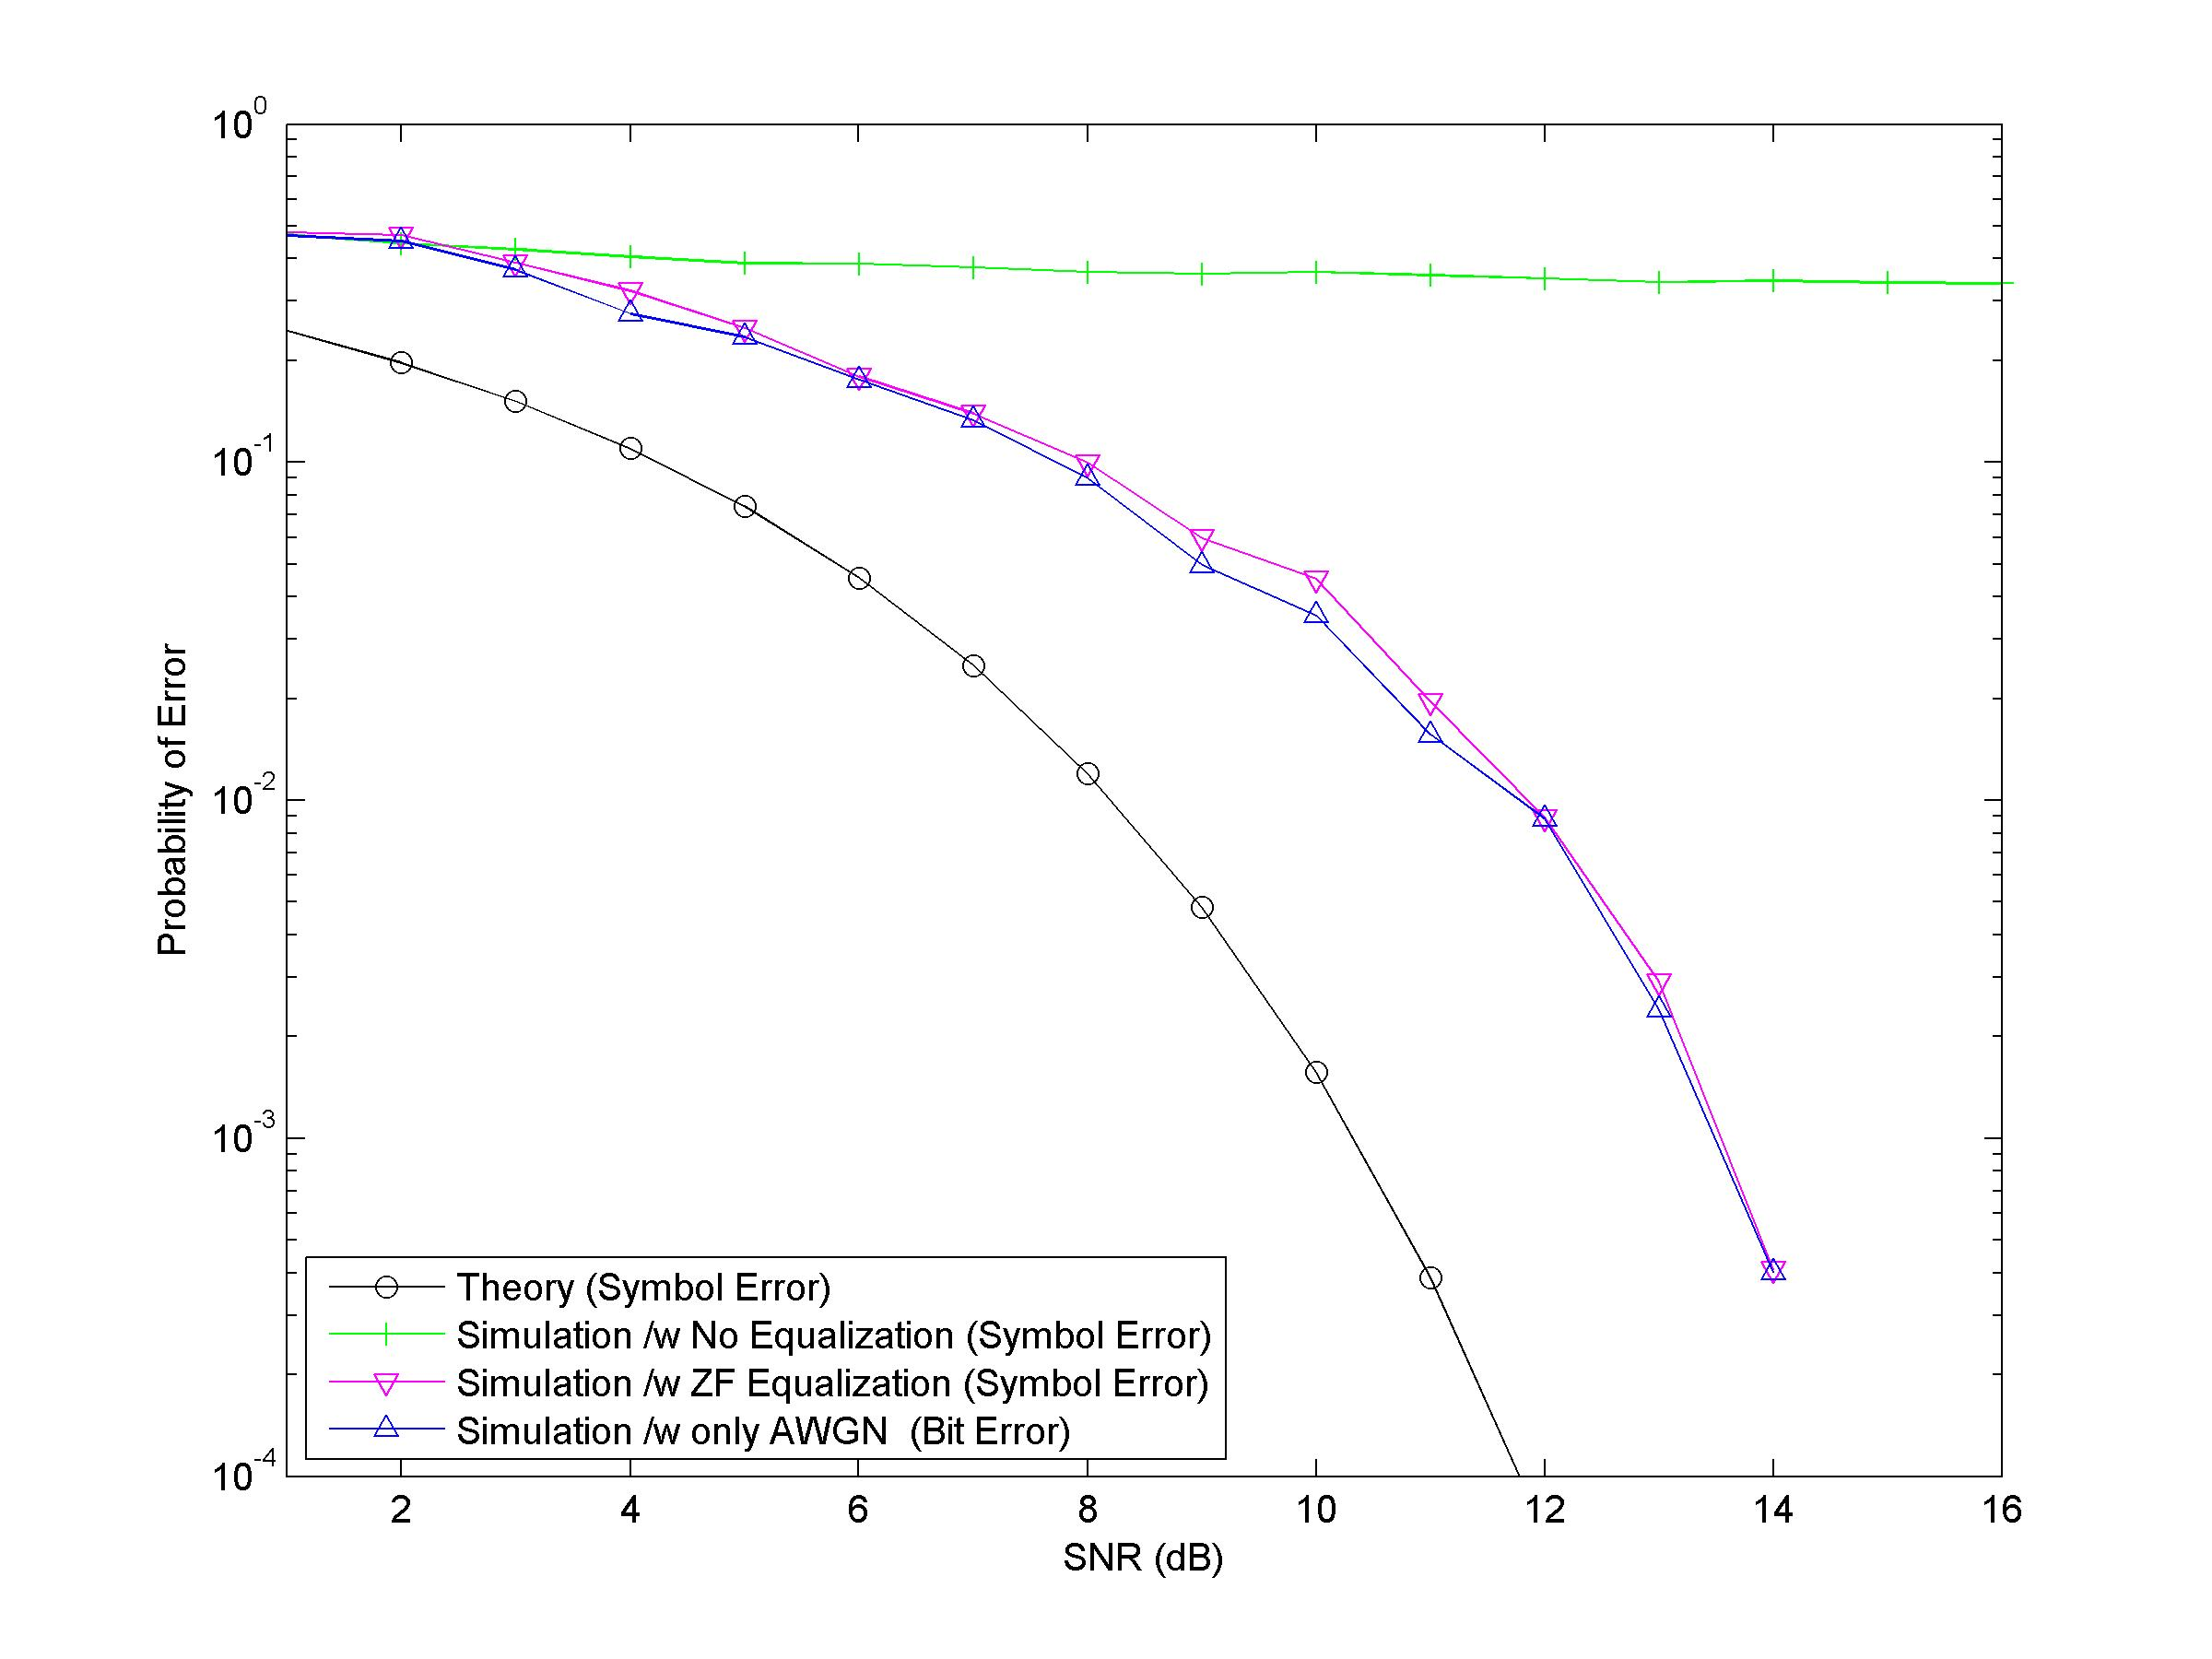
\includegraphics[width=0.8\textwidth]{qpSNR.jpg}
\caption{Probability of error graph for QPSK scheme, showing the results of different simulations done with no equalizer, with equalizer, with only AWGN, and the theoretical limit \label{fig:qpBER}}
\end{figure}

\begin{figure}[H]
\centering
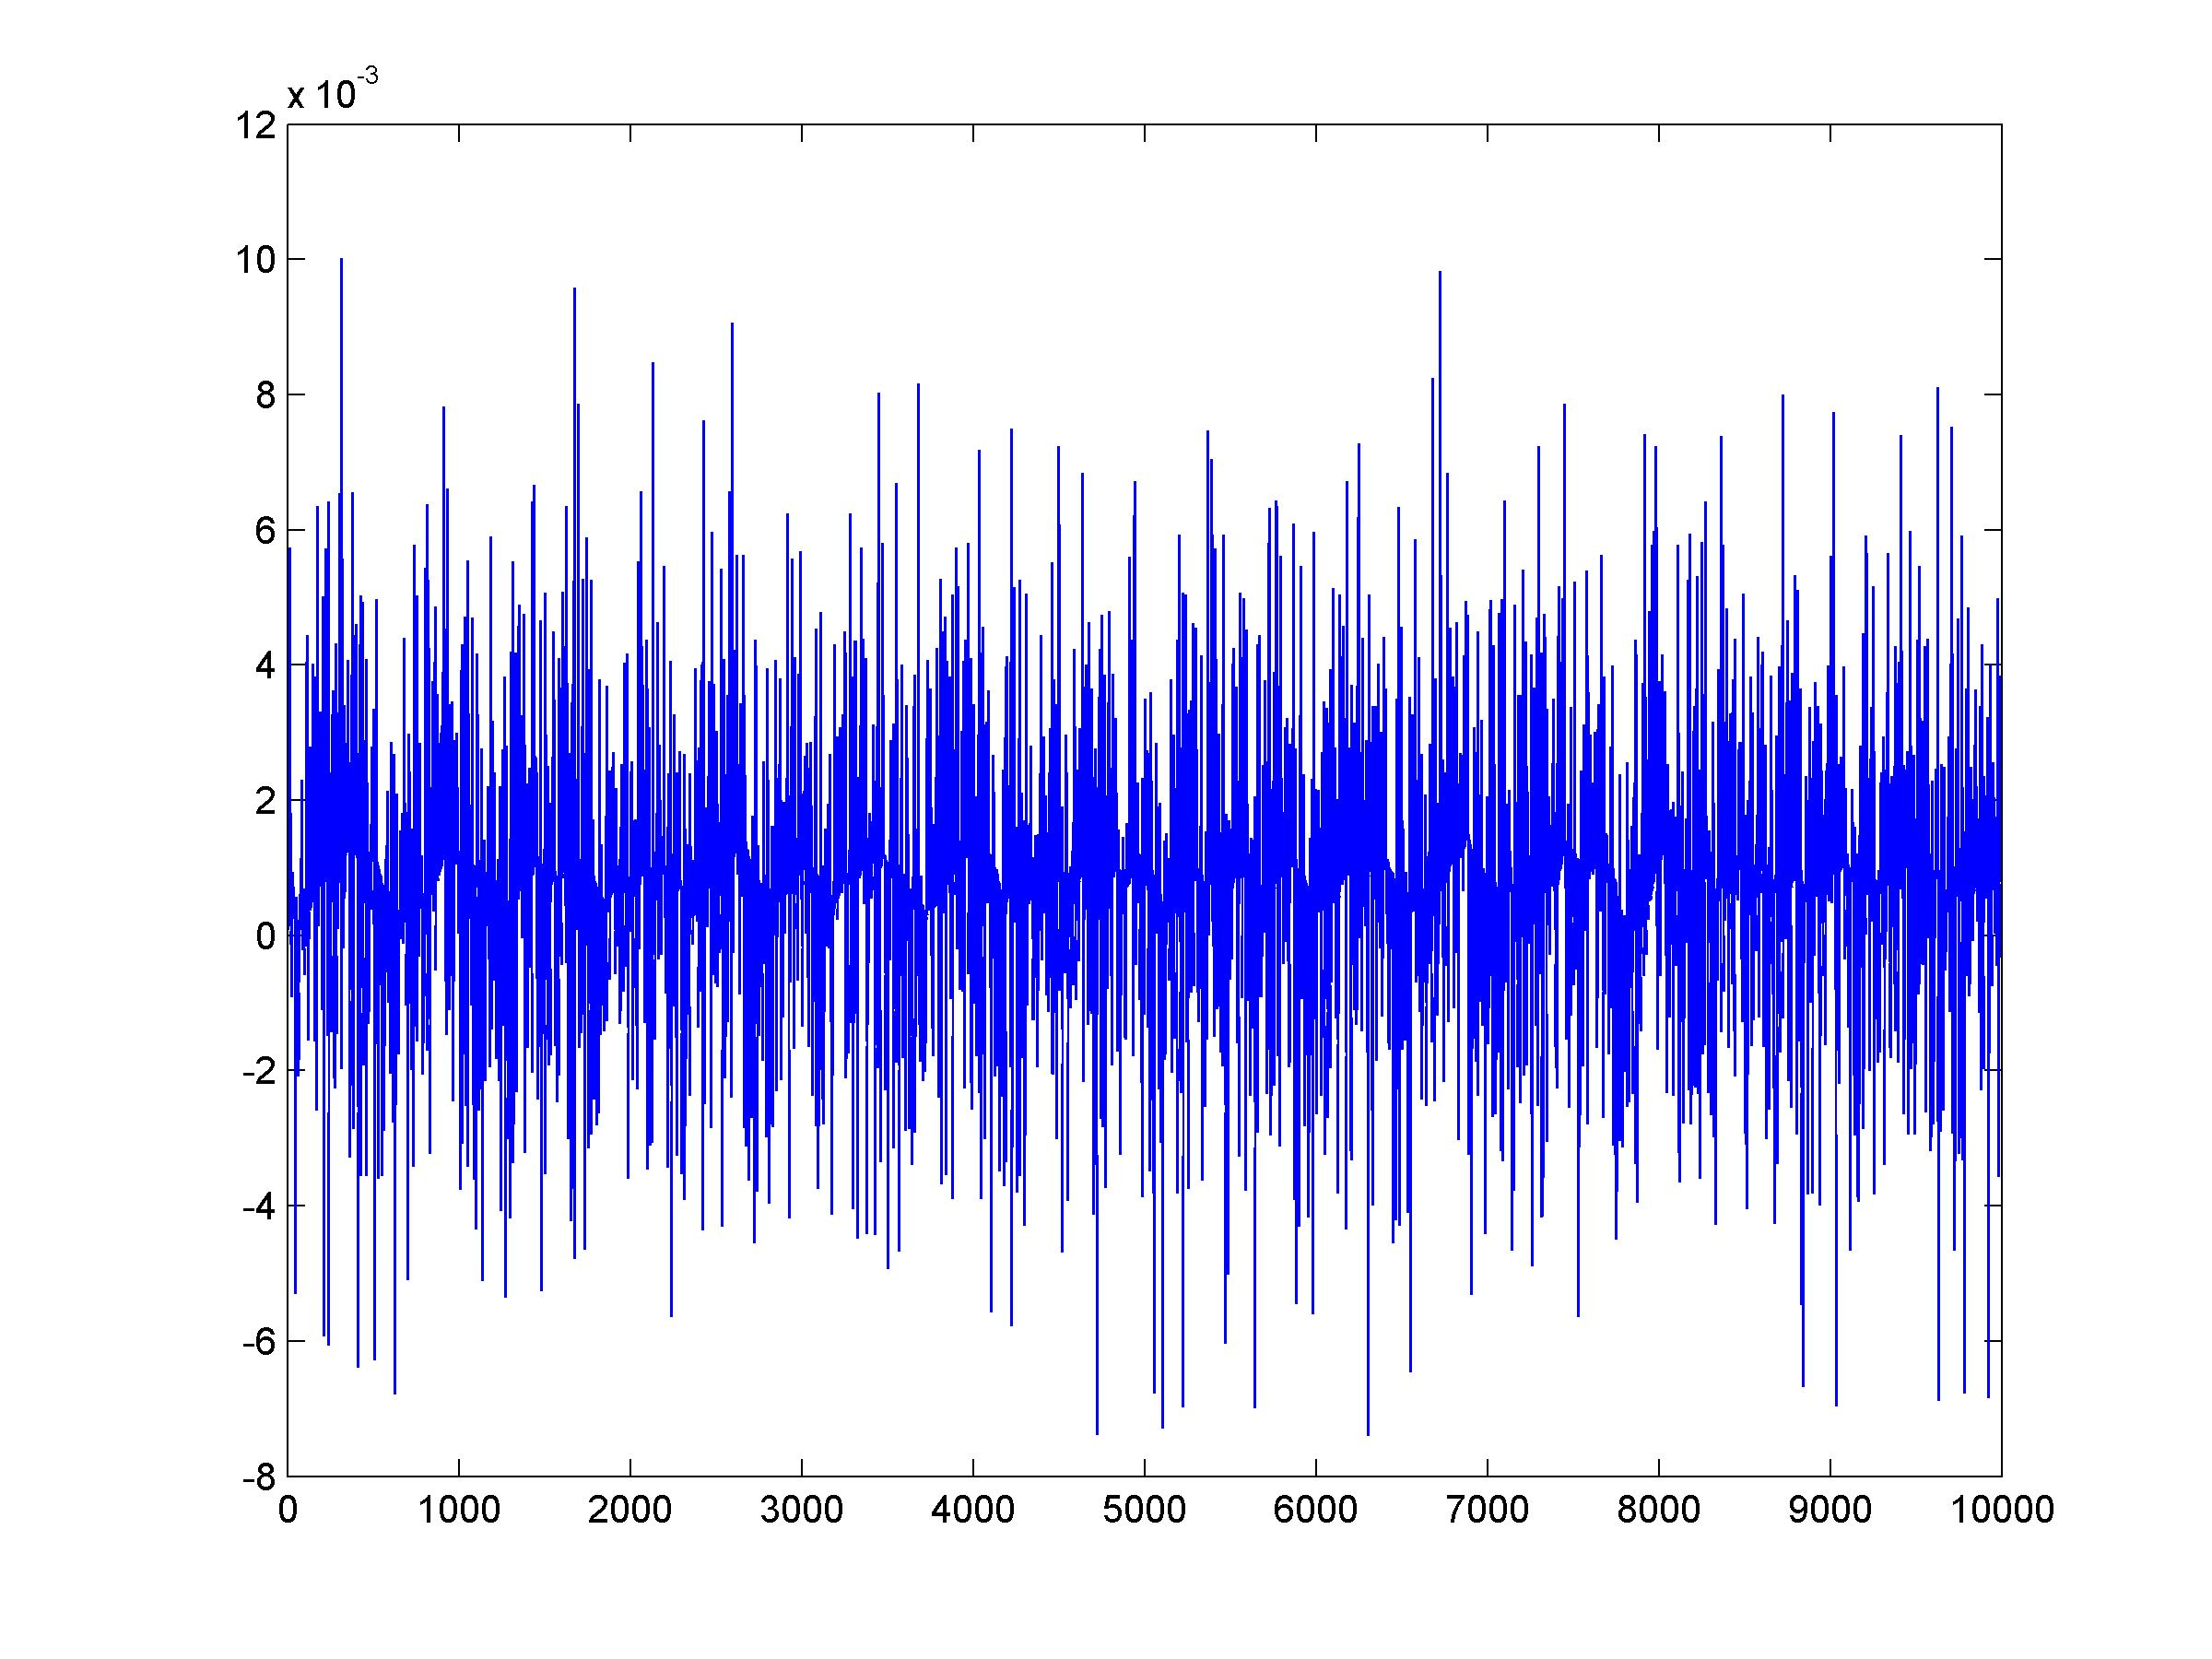
\includegraphics[width=0.8\textwidth]{loop_filter_qpsk20.jpg}
\caption{The output of the loop filter used in the Costas recovery loop.  This shows there is phase error between the local oscillator at RX-end and the incoming signal. Simulated at 20 dB SNR. \label{fig:qpLoop}}
\end{figure}

\begin{figure}[H]
\centering
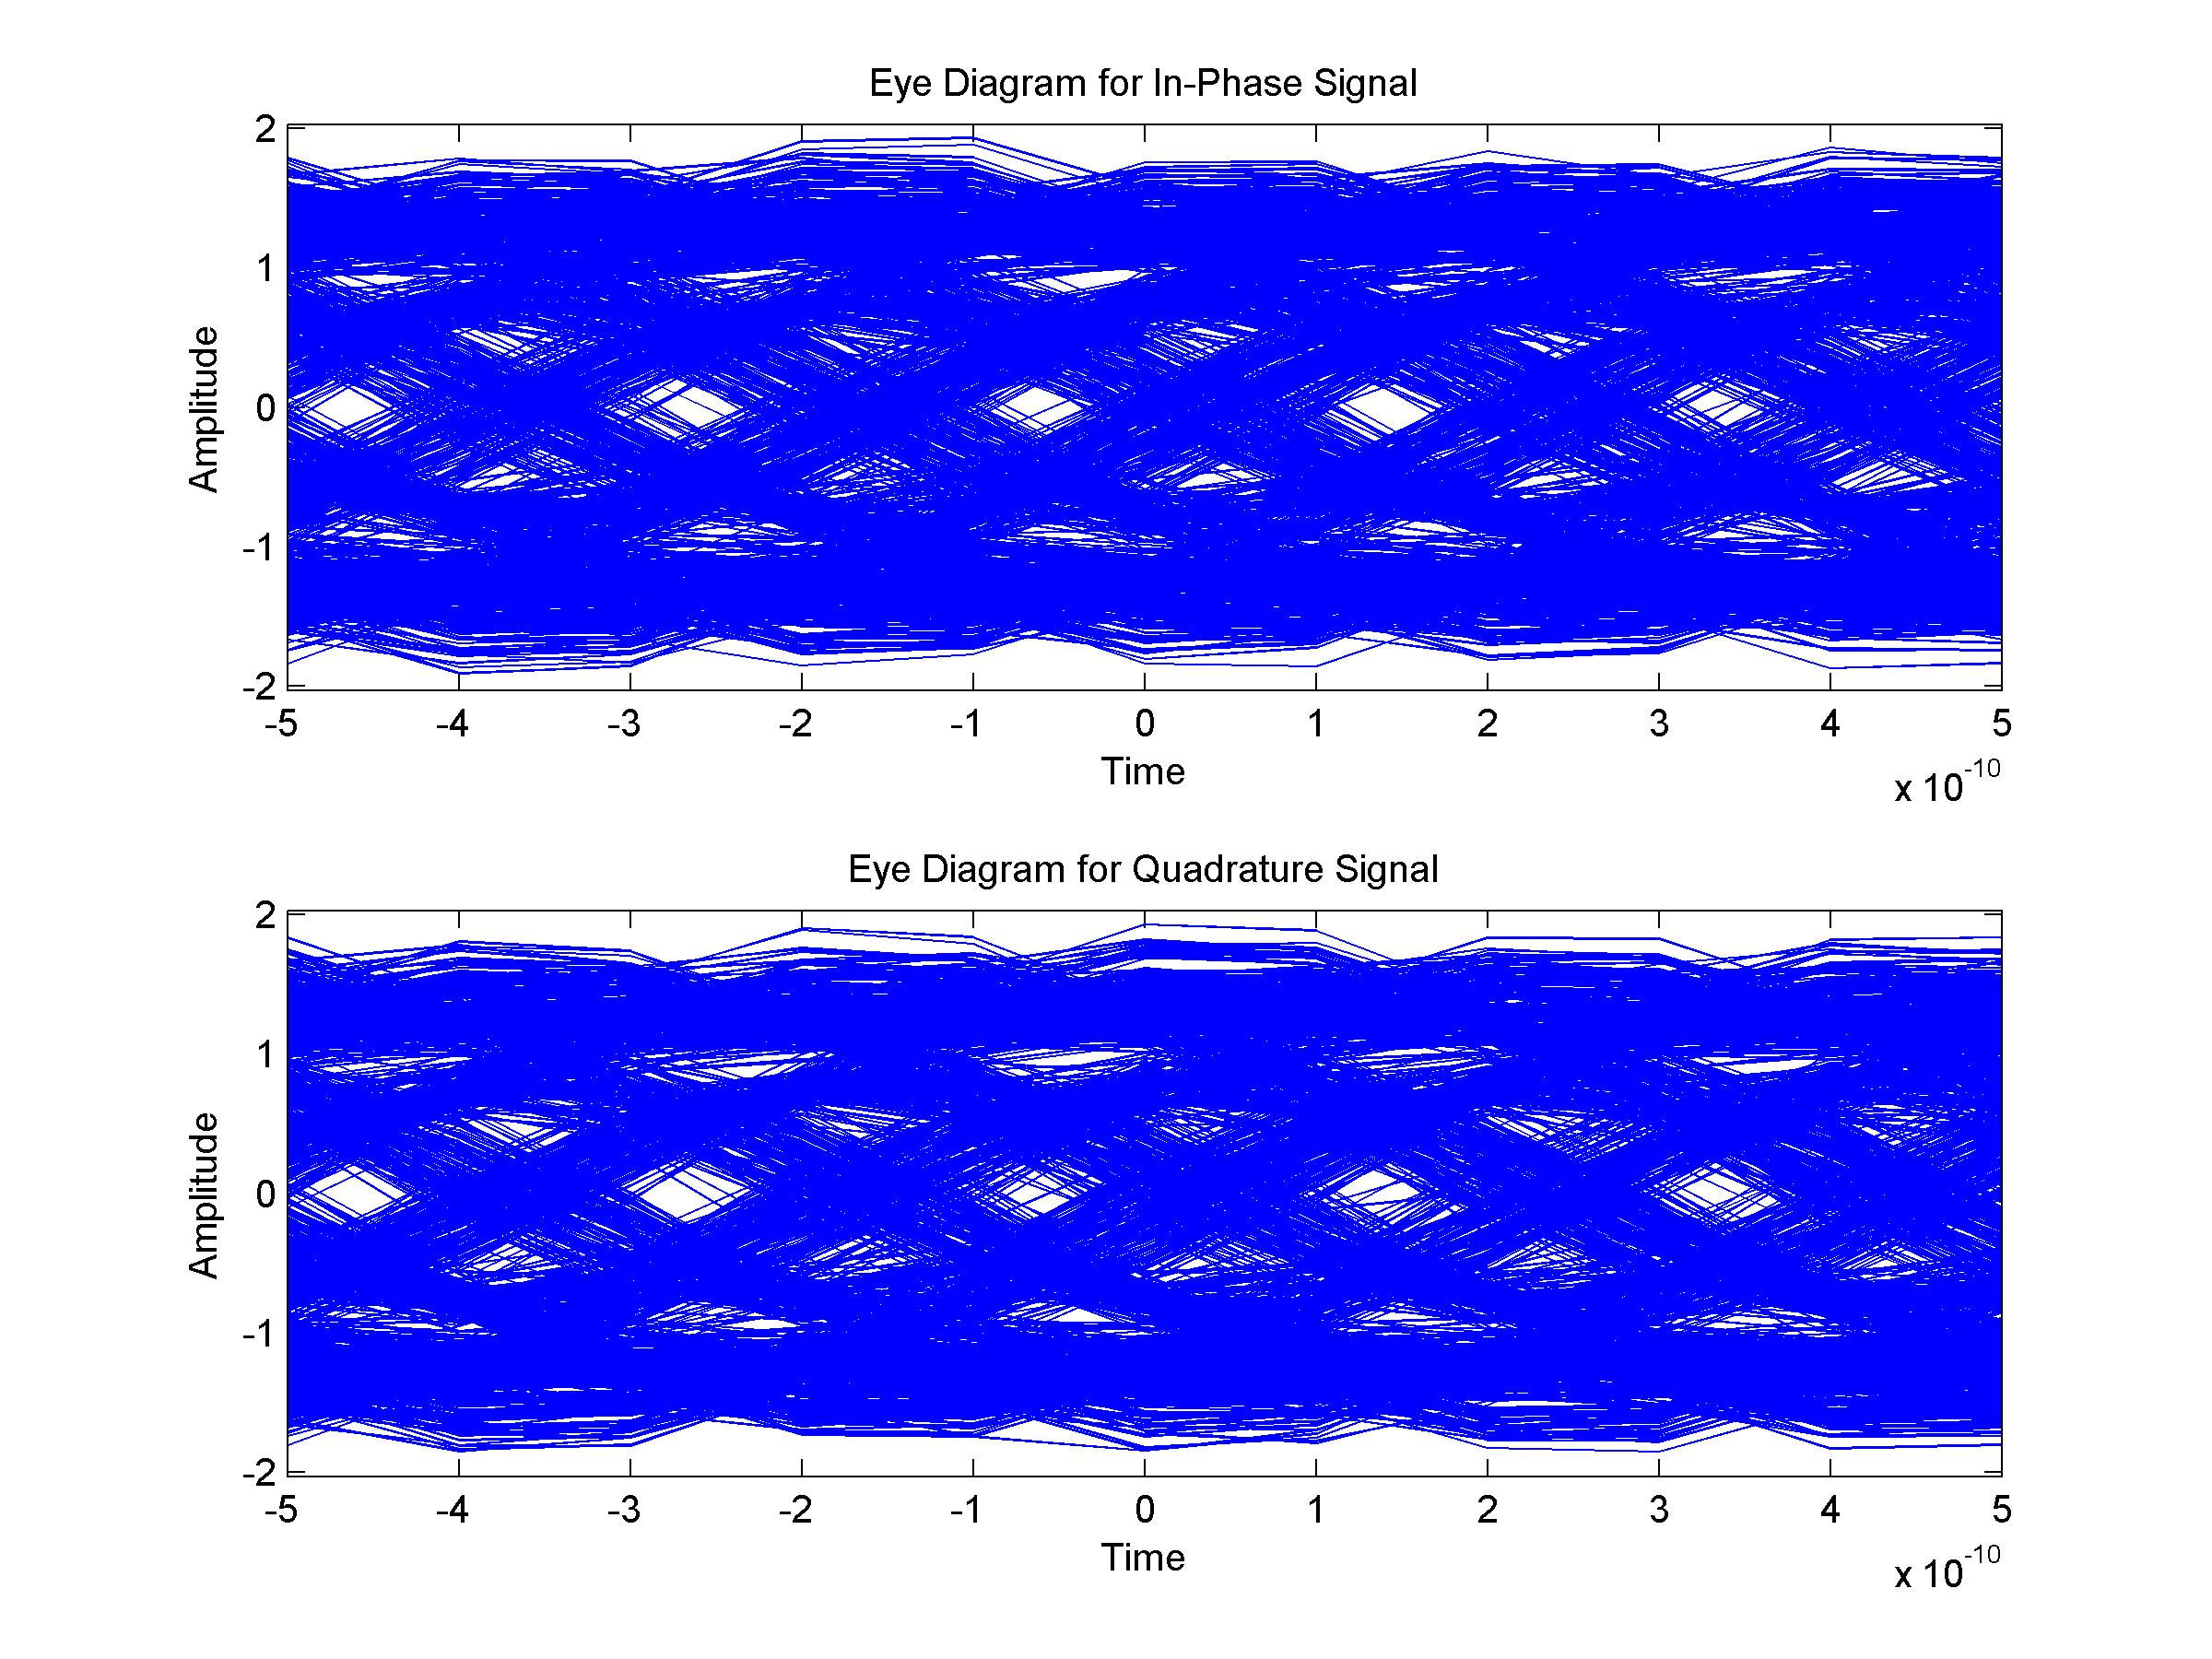
\includegraphics[width=0.8\textwidth]{matched_eye_qpsk20.jpg}
\caption{The eye-diagram of the output of the matched filter at RX-end under bandlimited channel condition is shown. Simulated at 20 dB SNR. \label{fig:qpEyeMatch}}
\end{figure}

\begin{figure}[H]
\centering
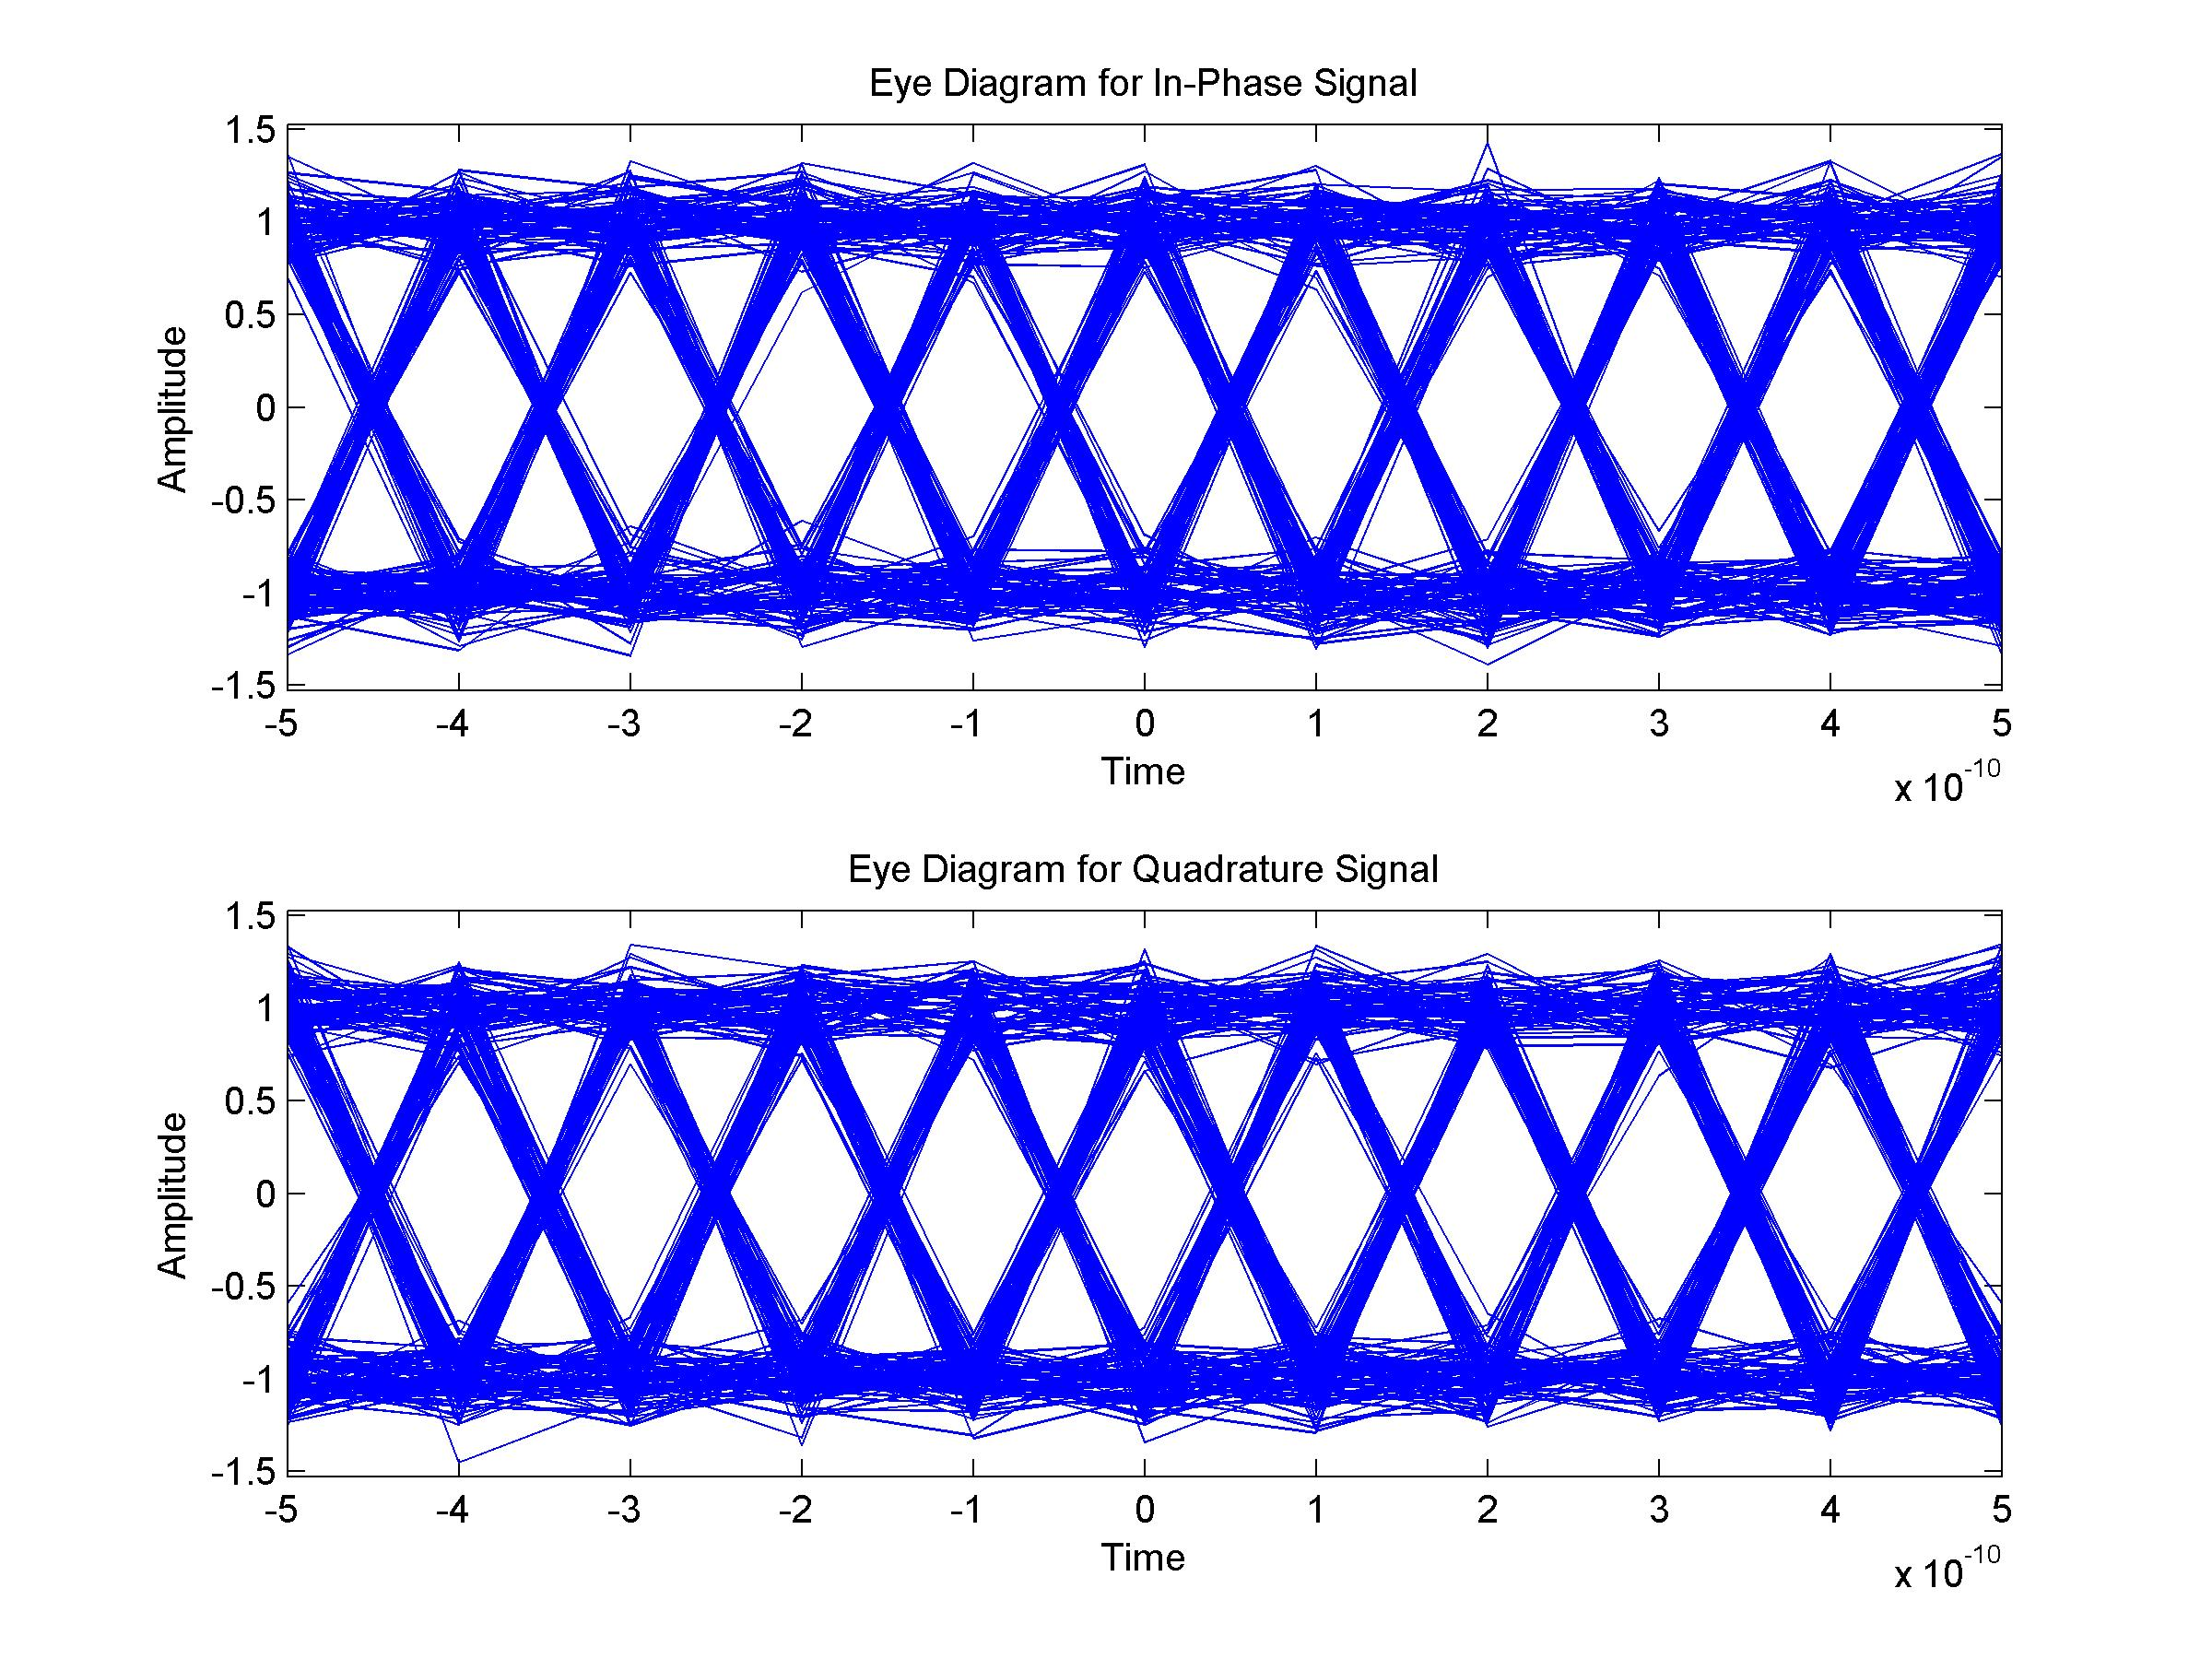
\includegraphics[width=0.8\textwidth]{equalized_eye_qpsk20.jpg}
\caption{ The eye-diagram of the output of the ZF equalizer at RX-end under bandlimited channel condition is shown. Simulated at 20 dB SNR.\label{fig:qpEyeEqu}}
\end{figure}


\begin{figure}[H]
\centering
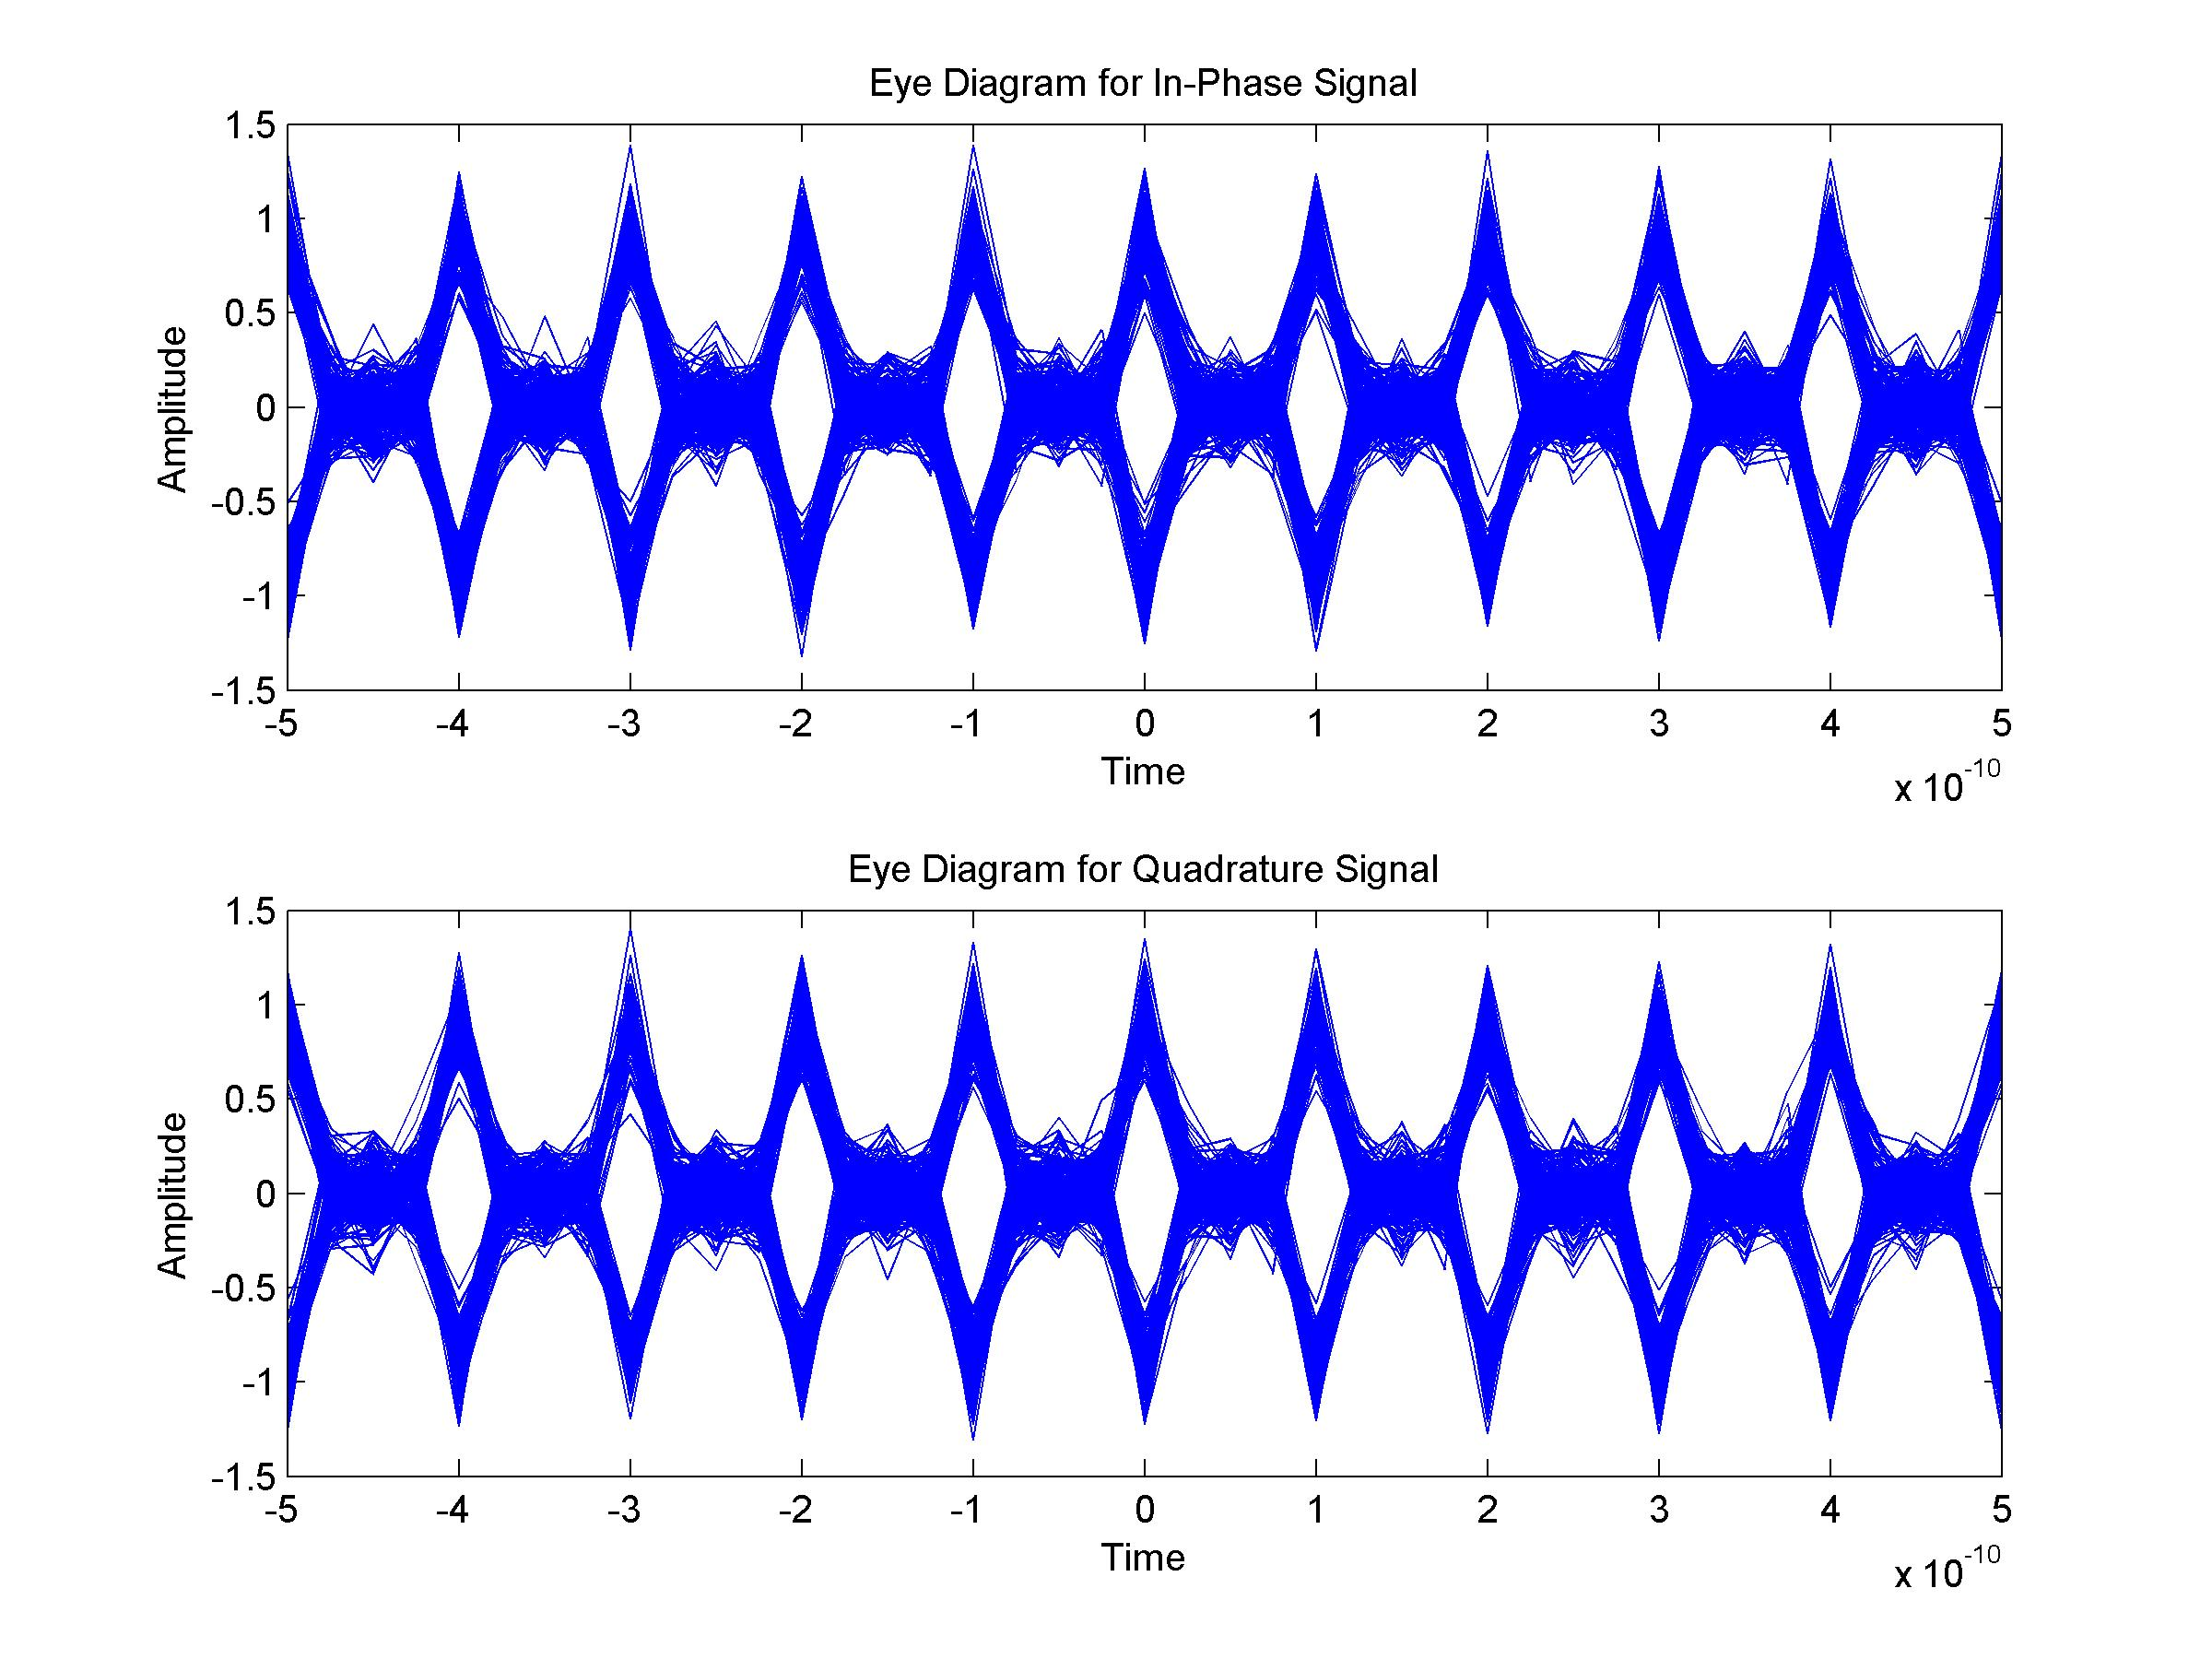
\includegraphics[width=0.8\textwidth]{awgn_eye_qpsk20.jpg}
\caption{The eye-diagram of the output of the matched filter at RX-end under AWGN condition is shown. Simulated at 20 dB SNR. \label{fig:qpEyeAWGN}}
\end{figure}

\subsection{16-QAM Scheme Results}

\begin{figure}[H]
\centering
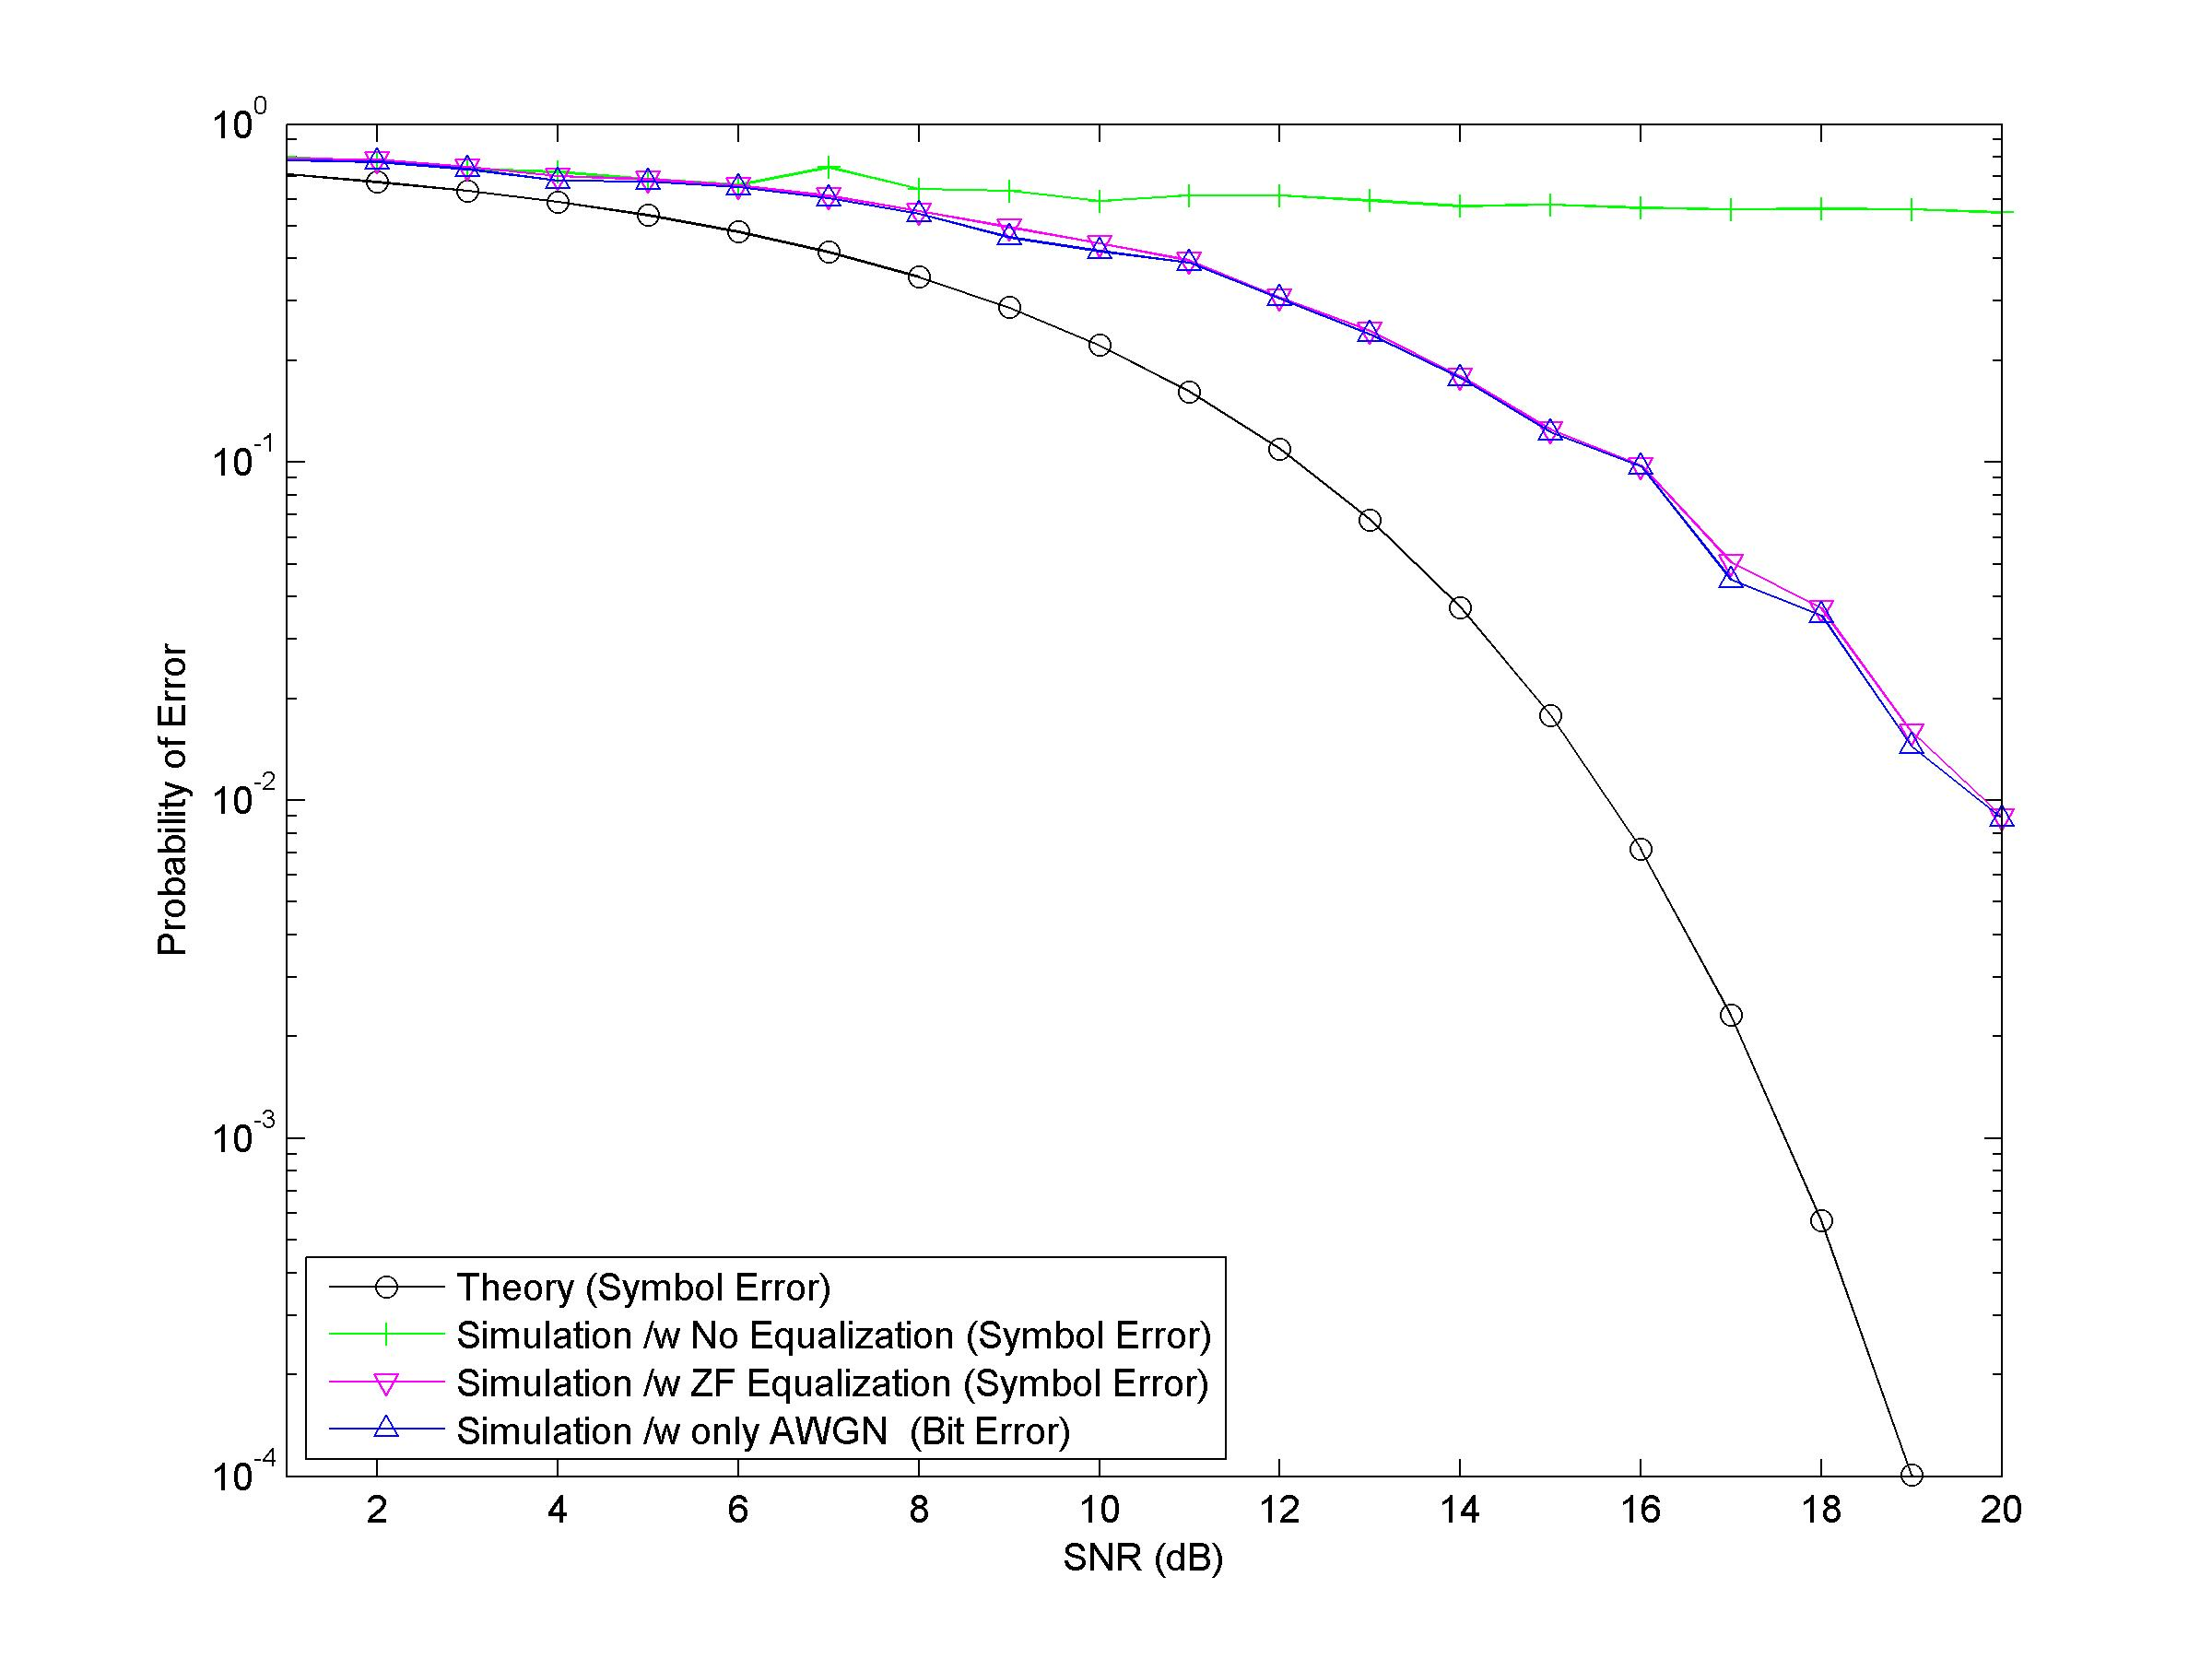
\includegraphics[width=0.8\textwidth]{qam16SNR.jpg}
\caption{Probability of Error graph for QPSK scheme, showing the results of simulations dones with no equalizer, with equalizer, with only AWGN, and the theoretical limit. \label{fig:qamBER}}
\end{figure}

\begin{figure}[H]
\centering
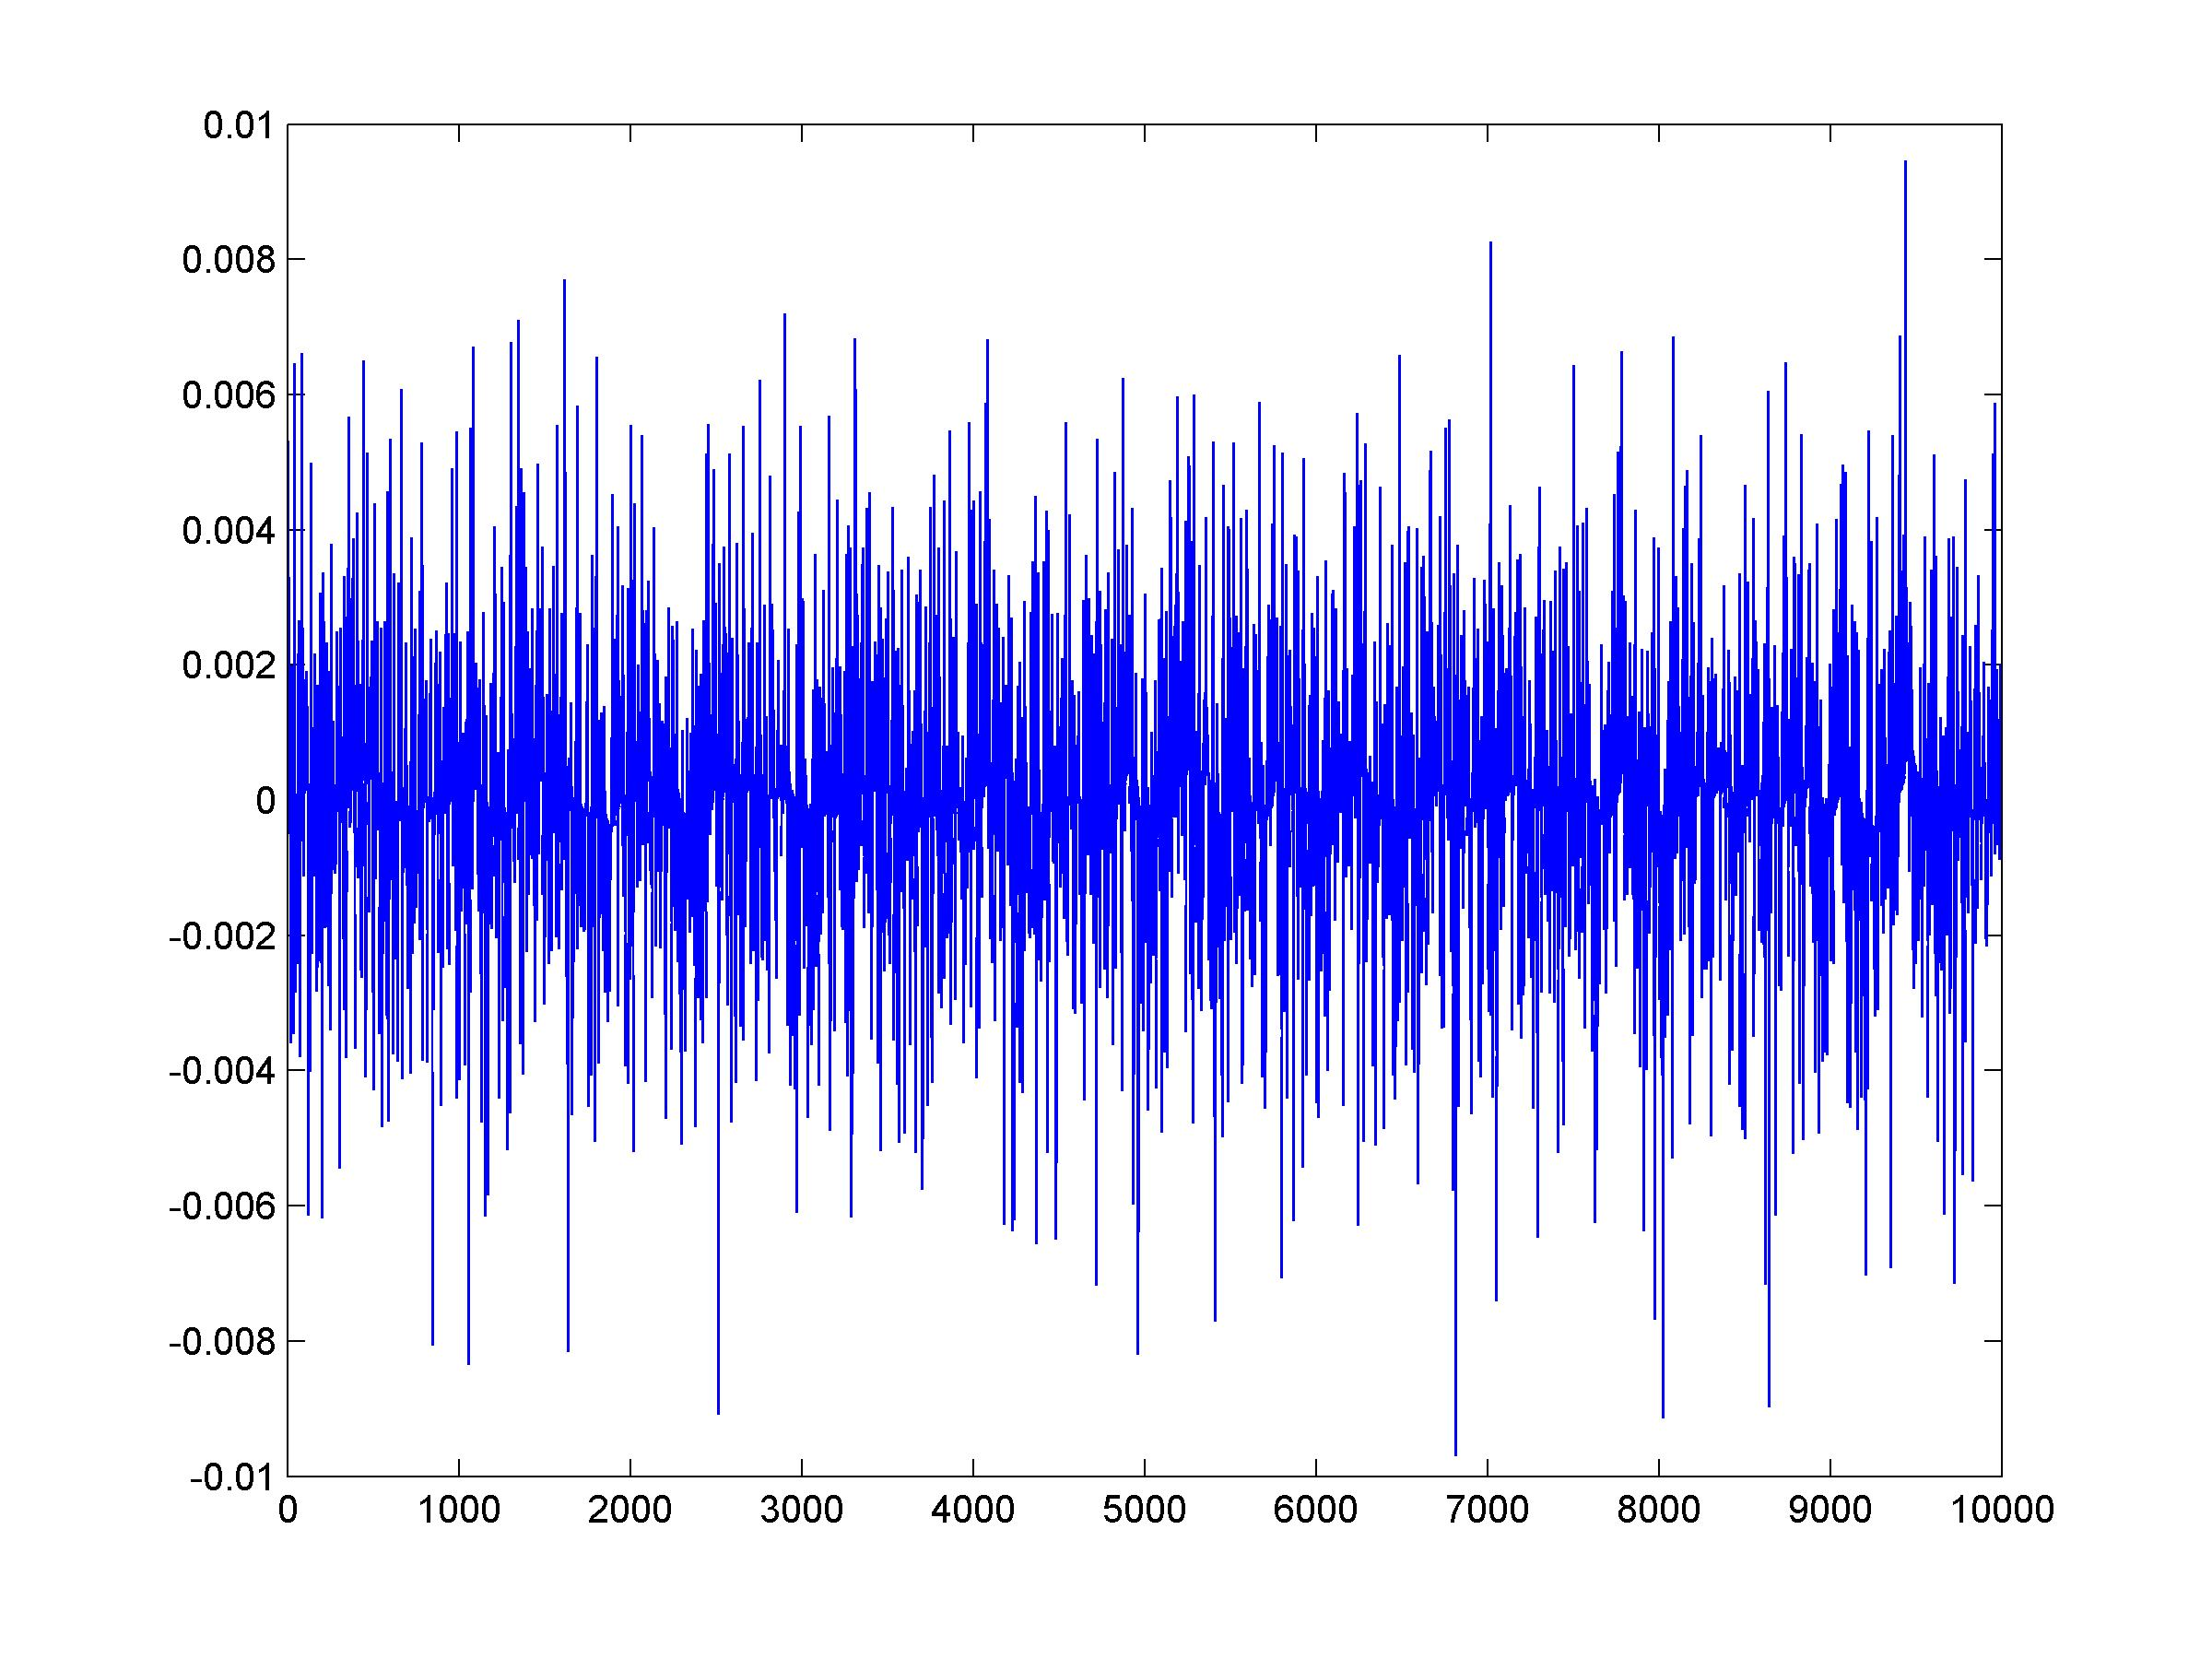
\includegraphics[width=0.8\textwidth]{loop_filter_qam20.jpg}
\caption{The output of the loop filter used in the Costas recovery loop.  This shows there is phase error between the local oscillator at RX-end and the incoming signal. Simulated at 20 dB SNR. \label{fig:qamLoop}}
\end{figure}

\begin{figure}[H]
\centering
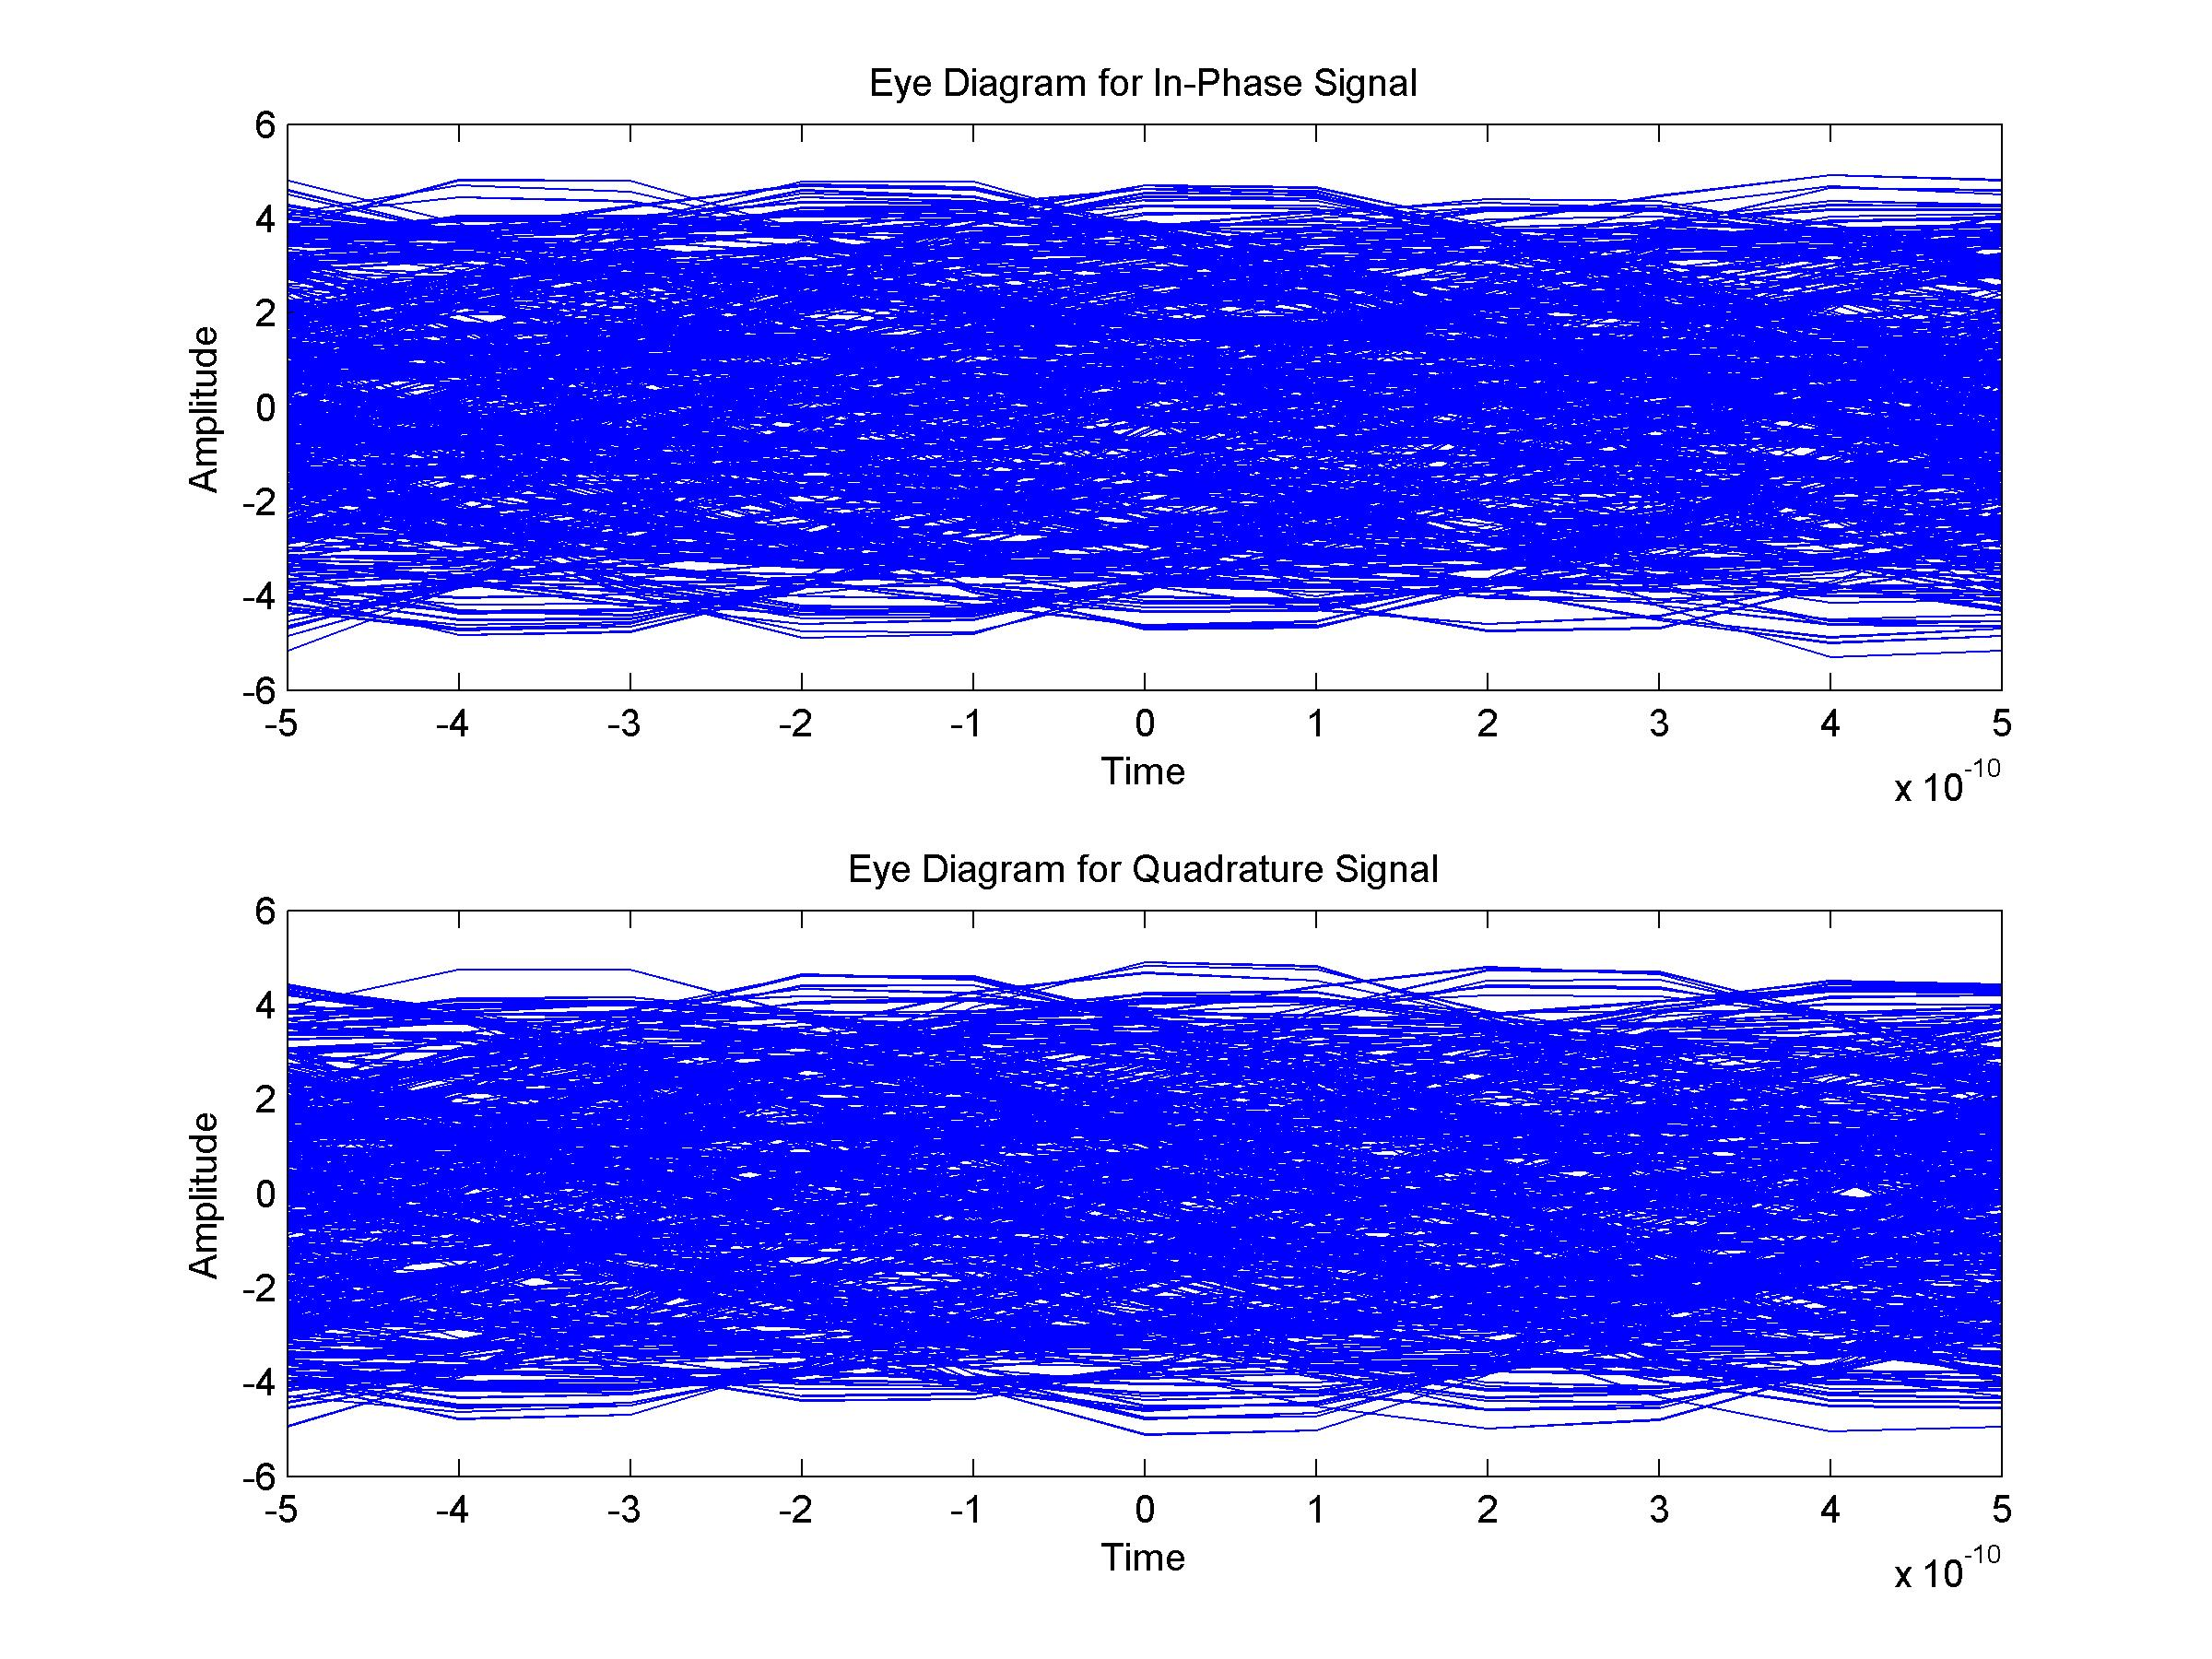
\includegraphics[width=0.8\textwidth]{matched_eye_16qam20.jpg}
\caption{The eye-diagram of the output of the matched filter at RX-end under bandlimited channel condition is shown. Simulated at 20 dB SNR. \label{fig:qamEyeMatch}}
\end{figure}

\begin{figure}[H]
\centering
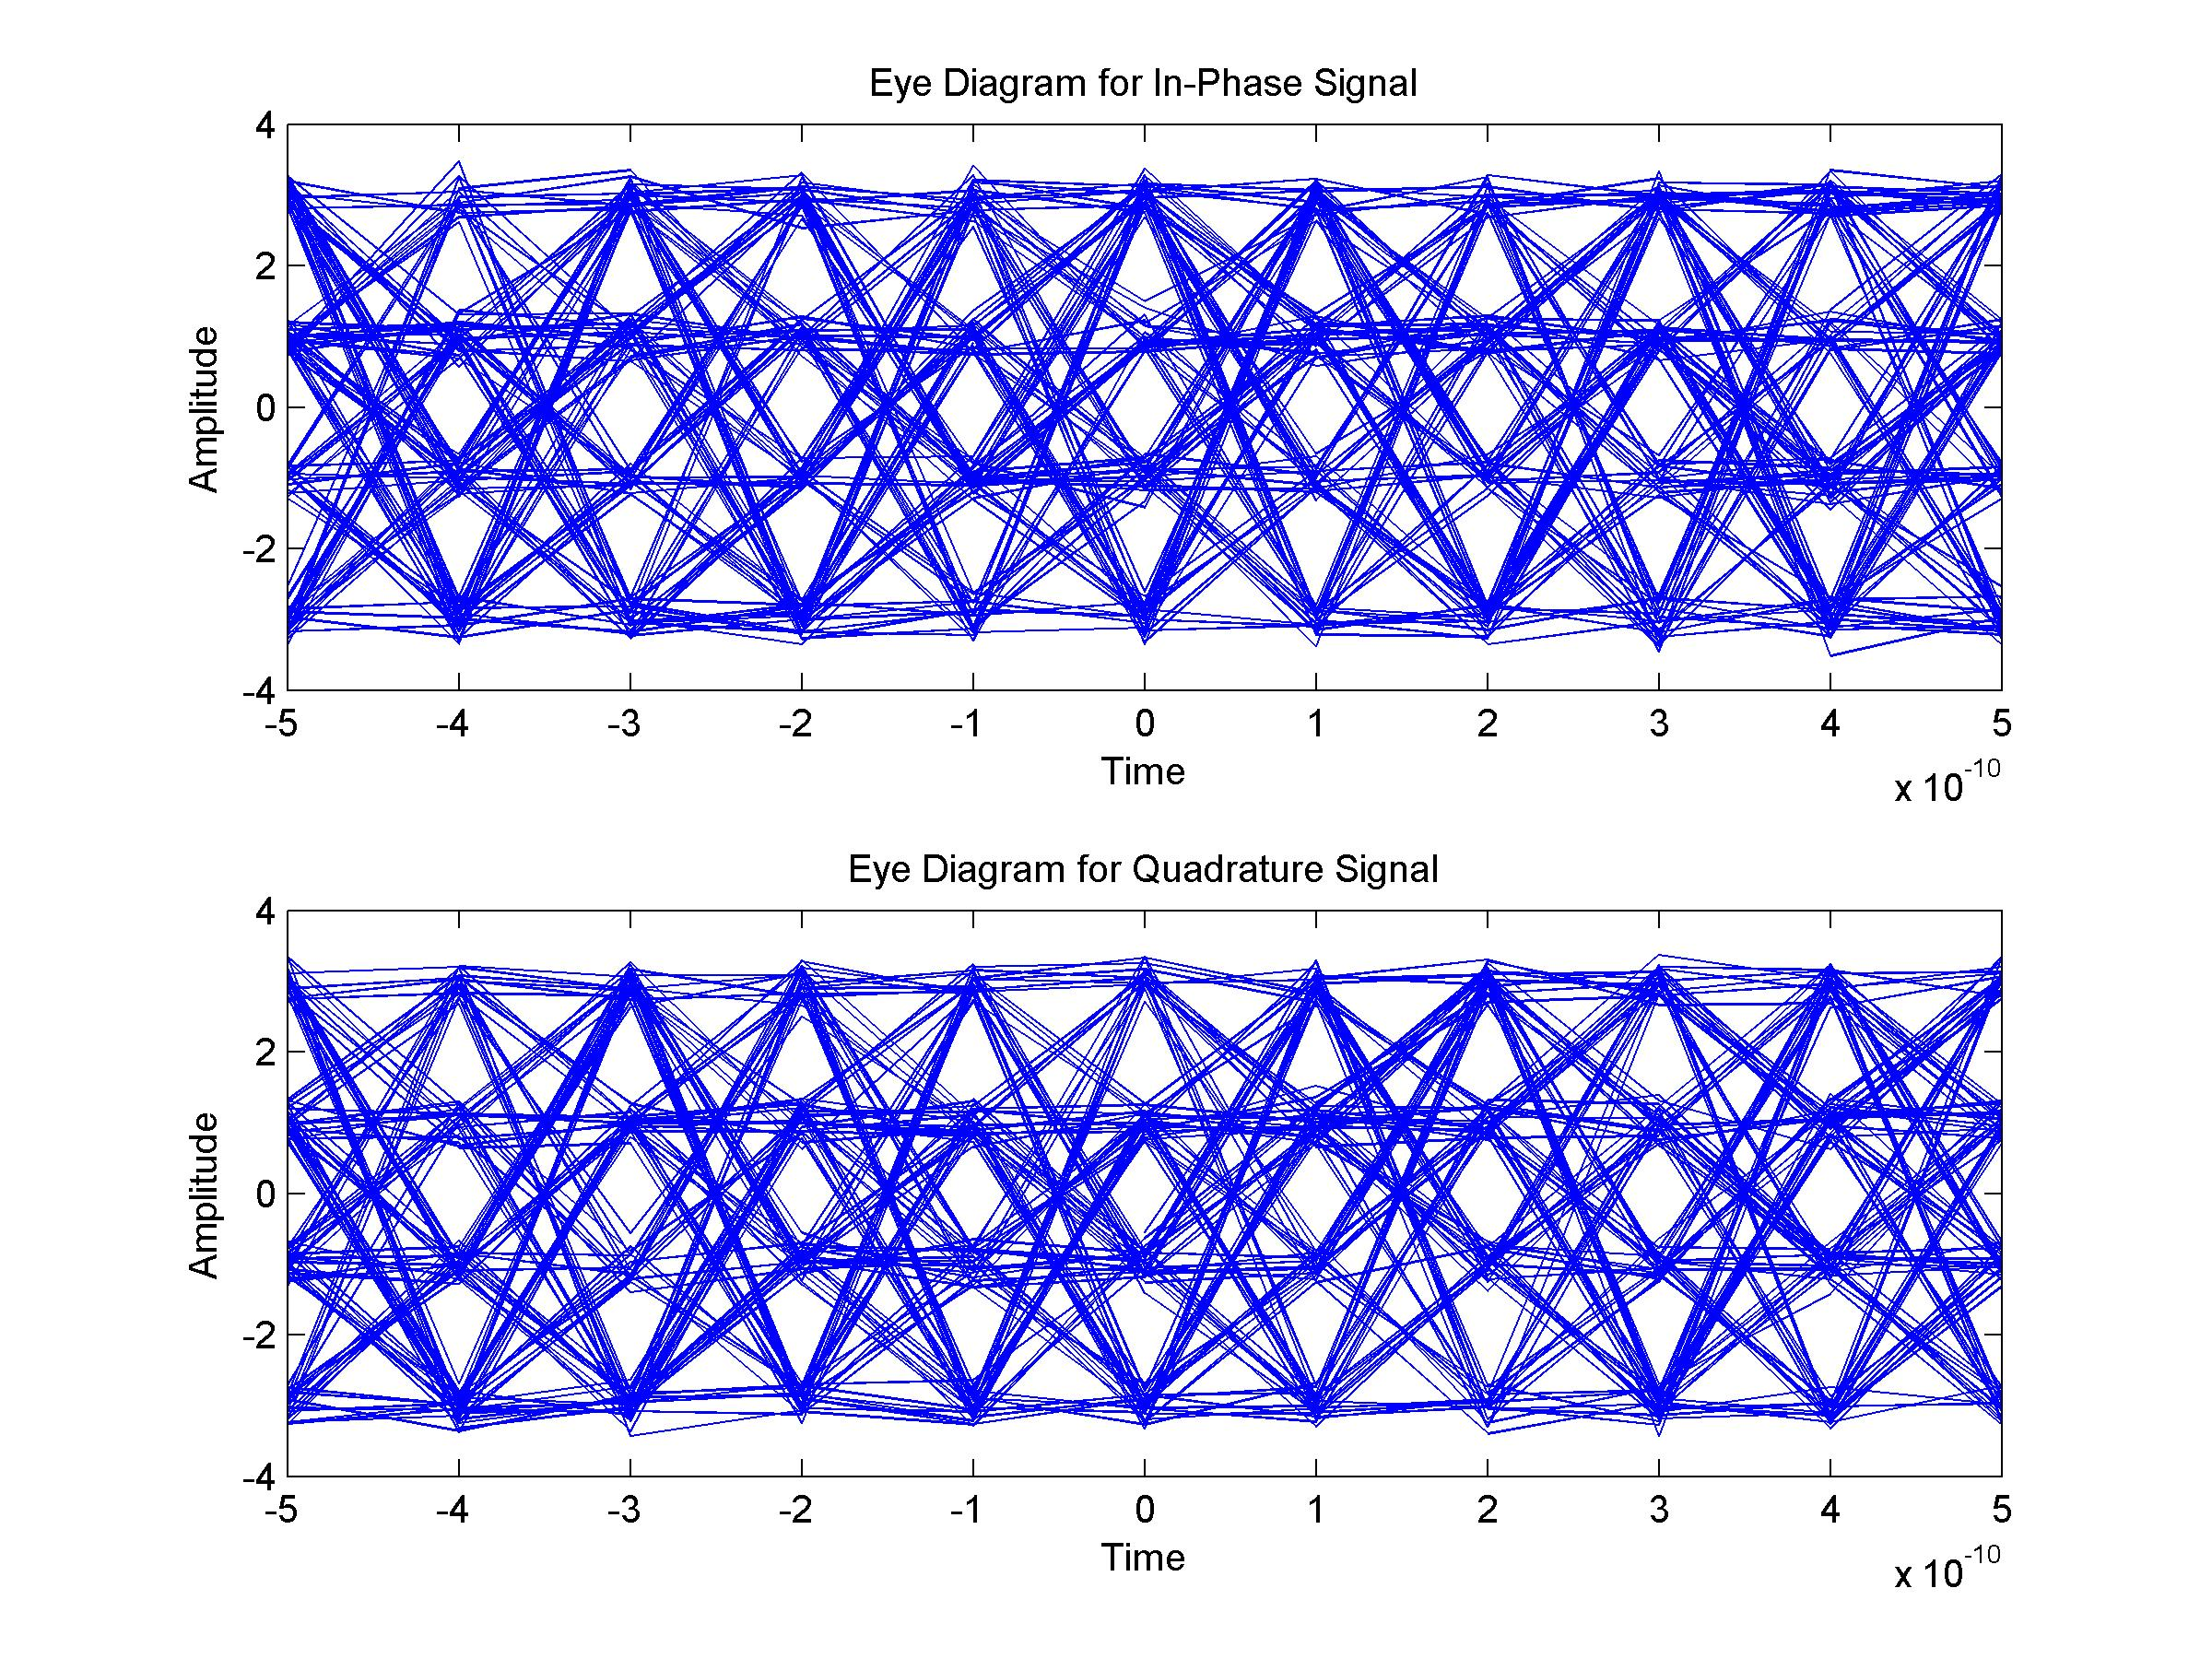
\includegraphics[width=0.8\textwidth]{equalized_eye_qam20.jpg}
\caption{The eye-diagram of the output of the ZF equalizer at RX-end under bandlimited channel condition is shown. Simulated at 20 dB SNR \label{fig:qamEyeEqu}}
\end{figure}

\begin{figure}[H]
\centering
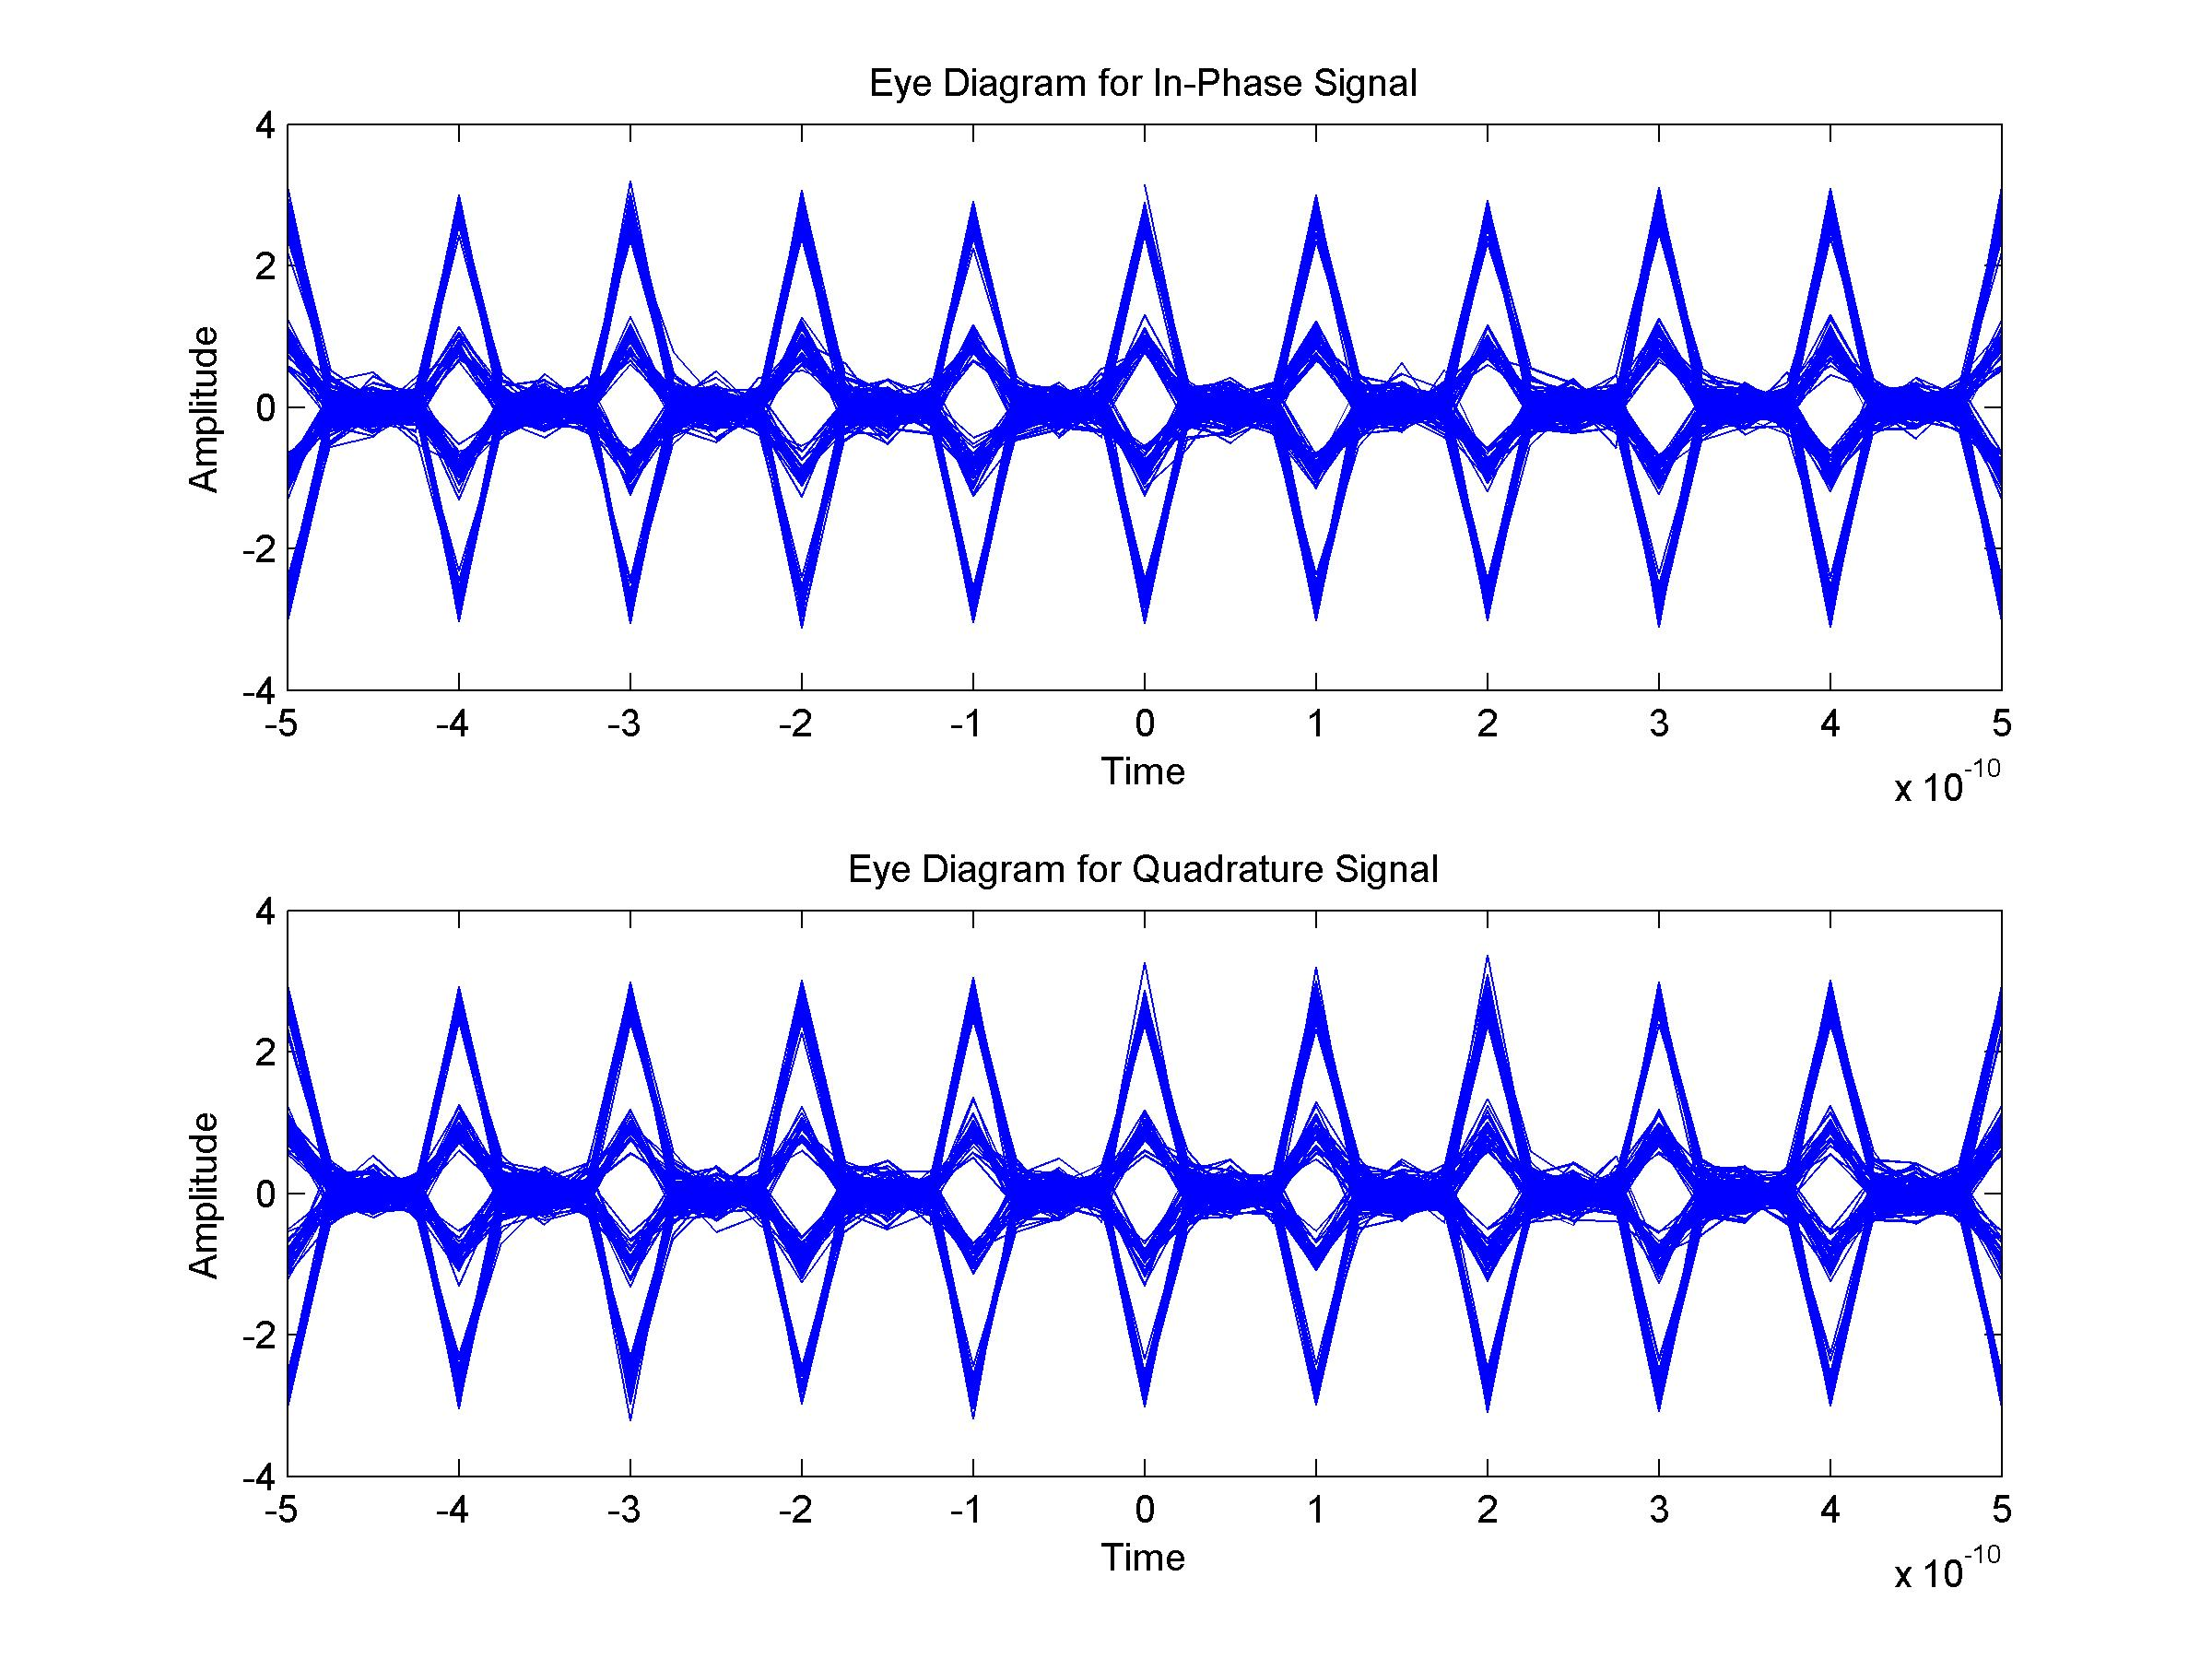
\includegraphics[width=0.8\textwidth]{awgn_eye_qam20.jpg}
\caption{The eye-diagram of the output of the matched filter at RX-end under AWGN condition is shown. Simulated at 20 dB SNR.\label{fig:qamEyeAWGN}}
\end{figure}

\newpage
\section{Conclusion}
\label{sec:conc}
The purpose of this project was to simulate a communication link and send a signal with 10MHz bandwidth using QPSK/16QAM modulation schemes over a bandlimited channel with AWGN and impulse response  $h(t) = 0.1\delta(t + 100 \mathtt{ns}) + 0.8\delta(t -40 \mathtt{ns}) + 0.95\delta(t - 30 \mathtt{ns}) + 0.7\delta(t - 100 \mathtt{ns}) - 0.35\delta(t - 170 \mathtt{ns})$. \\

In addition, to make the simulation realistic, some impairments are introduced to the system.  The effect of these errors are dealt with and studied.  These impairments are:
\begin{itemize}
\item Pulse Shaping and its effects on ISI.
\item Frequency/Phase Offset between RX osciallator and received signal and its effects on the efficiency of the system.
\item Phase error recovery loops and their effect on the efficiency of the system.
\item Response of Bandlimited channels and their effect on ISI.
\item AWGN channel and its effects on the efficiency of the system
\item Bandlimited channel equalizers and their effect on ISI cancellation
\item DAC/ADC converters and the effect of different LPF cut-off frequencies and sampling delays on the efficiency of the system  
\end{itemize}

In order to realize this system and simulate it, the block diagram in Figure~\ref{fig:system} was implemented and results of the simulations are given in Section~\ref{sec:results}.

From the analysis of these results, we can deduce the following conclusions about our communication system:
\begin{itemize}
\item Looking at the probability of error rate graphs for both QPSK and 16-QAM schemes given in Figures~\ref{fig:qpBER} and~\ref{fig:qamBER}, we see that the theoretical limits form a lower bound and our simulations cannot reach this lower bound. There is almost a 3dB difference (at high SNR values) between the theoretical limit and the simulations with equalizers for both QPSK and 16-QAM. This is caused by the fact that we are using A/D and D/A converters in our system. Although the results obtained are fairly close to the theoretical values, they can never achieve the limit due to the fact that we need infinite over-sampling to construct an analog signal from a digital signal. 

Furthermore, the success of the system with only AWGN and with equalizers handling ISI are almost the same. This was expected since the equalizer is designed to cancel out the ISI effect of the bandlimited channel.  The fact that the two scenarios perform comparably indicates the ZF equalizer is working correctly.  

On the other hand, the when the system is left without equalization, the performance is terrible.  An error on the order of .1 is not suitable for communication.  The effects of ISI sufficiently muddle the received signal so that it cannot be recovered without equalization. 

\item The objective of the Costas Loop is to recover and track out any phase or frequency offsets that might be present in the received signal.  The integral feedback handles the phase error between the local oscillator at the receiver and the incoming signal.  

The Figures~\ref{fig:qamLoop} and~\ref{fig:qpLoop}, both at 20dB SNR, show the feedback filter tracks to zero the phase error.  The settling time is BLAH.  This is sufficient for our stetting.  The response structure exists in the lower SNR case, but the settling time happens in only a few samples and gets lost in the plot.  Note that the noise level sits around zero. 

By setting the loop filter coefficients to the right values and increasing the sampling rate, we can improve the settling time, [Section~\ref{sec:issues}]. The loop filter output graphics prove this result: the frequency error estimate converges to steady state very fast. This also means that we don't really need to throw any of the received bits.

\item Looking at the eye-diagrams of the matched filter output, shown in Figures~\ref{fig:qamEyeMatch} and~\ref{fig:qpEyeMatch}, we observe that there are no "eyes" present at the sampling points $T_s$. This shows that the system has a very poor performance if no equalization block is present at the RX-end. This conclusion is supported by the Probability of Error Rate graph of the system with no equalization. \\

On the other hand, in the eye-diagrams of the equalizer output the "eye" structures are evident [Figures~\ref{fig:qamEyeEqu} and~\ref{fig:qpEyeEqu}].  At the sampling points $T_s$, it is clear there are four possible constellation points for 16-QAM and two possible constellation points for QPSK.  This nice alignment makes the signal demodulation in the case with an equalizer painless as compared to the case without equalization.  \\

Furthermore, the eye-diagrams of the AWGN-only system make a reference point for the system with bandlimited channel.  We expect close similarities between the eye diagram of the equalizer outputs and the matched filter outputs under only AWGN.  These are shown in Figures~\ref{fig:qamEyeAWGN} and~\ref{fig:qpEyeAWGN}. 
\end{itemize}



\section{Future Work}
\label{sec:future}
In the future, the system modified in order to both improve the results and enhance realism of the model. \\

In order to make the system more realistic, a colored gaussian noise channel might be used. As the implementation requires only one extra block, a whitening filter could then also be added to deal with the coloring. \\

Alternatively, the oversampling rate of the digital to analog conversion could be increased.  Increased bandwidth would improve the performance of the system by doing a better job moving between the analog and digital signals.   Increasing the oversampling rate would bring the performance closer to the theoretical limit.  Doing so, while beneficial to the conversion, would increase the processing time of the model.  We chose sufficient oversampling rate to accurately model the analog anti-aliasing filters, yet not so excessive that the simulation speed is compromised. \\

Another improvement to the system would be using a Minimum Mean Square Error Decision Feedback Equalizer (MMSE-DFE) equalizer instead of the ZF equalizer.  The noise enhancement danger, present in any Zero Forcing equalizer, is  dealt with by the use of mean square error optimization in a feedback loop.  Although adding a feedback loop at the equalizer would mean more complexity, the MMSE-DFE would improve performance if noise enhancment became a problem.  \\

Finally, instead of a phase tracker, a frequency tracker could be used in the Costas Loop to handle the frequency offset.  Instead of using two integrators to hande the error, a gamble since the settling time of the loop may not be able to deal with frequencies above a certain level, the system could use a different loop to directly approximate the frequency error.  This would make the system more robust to higher frequency offsets since the error metric would then be Type 0 [See Appendix~\ref{app:feedback}].  In this case, we would no longer need to use a relatively large sampling period compared to the frequency offset.  


\appendix
\newpage
\bibliographystyle{plain}
\bibliography{final}
\newpage
% the \\ insures the section title is centered below the phrase: Appendix B
\section{Project Assignment}
\label{app:assign}
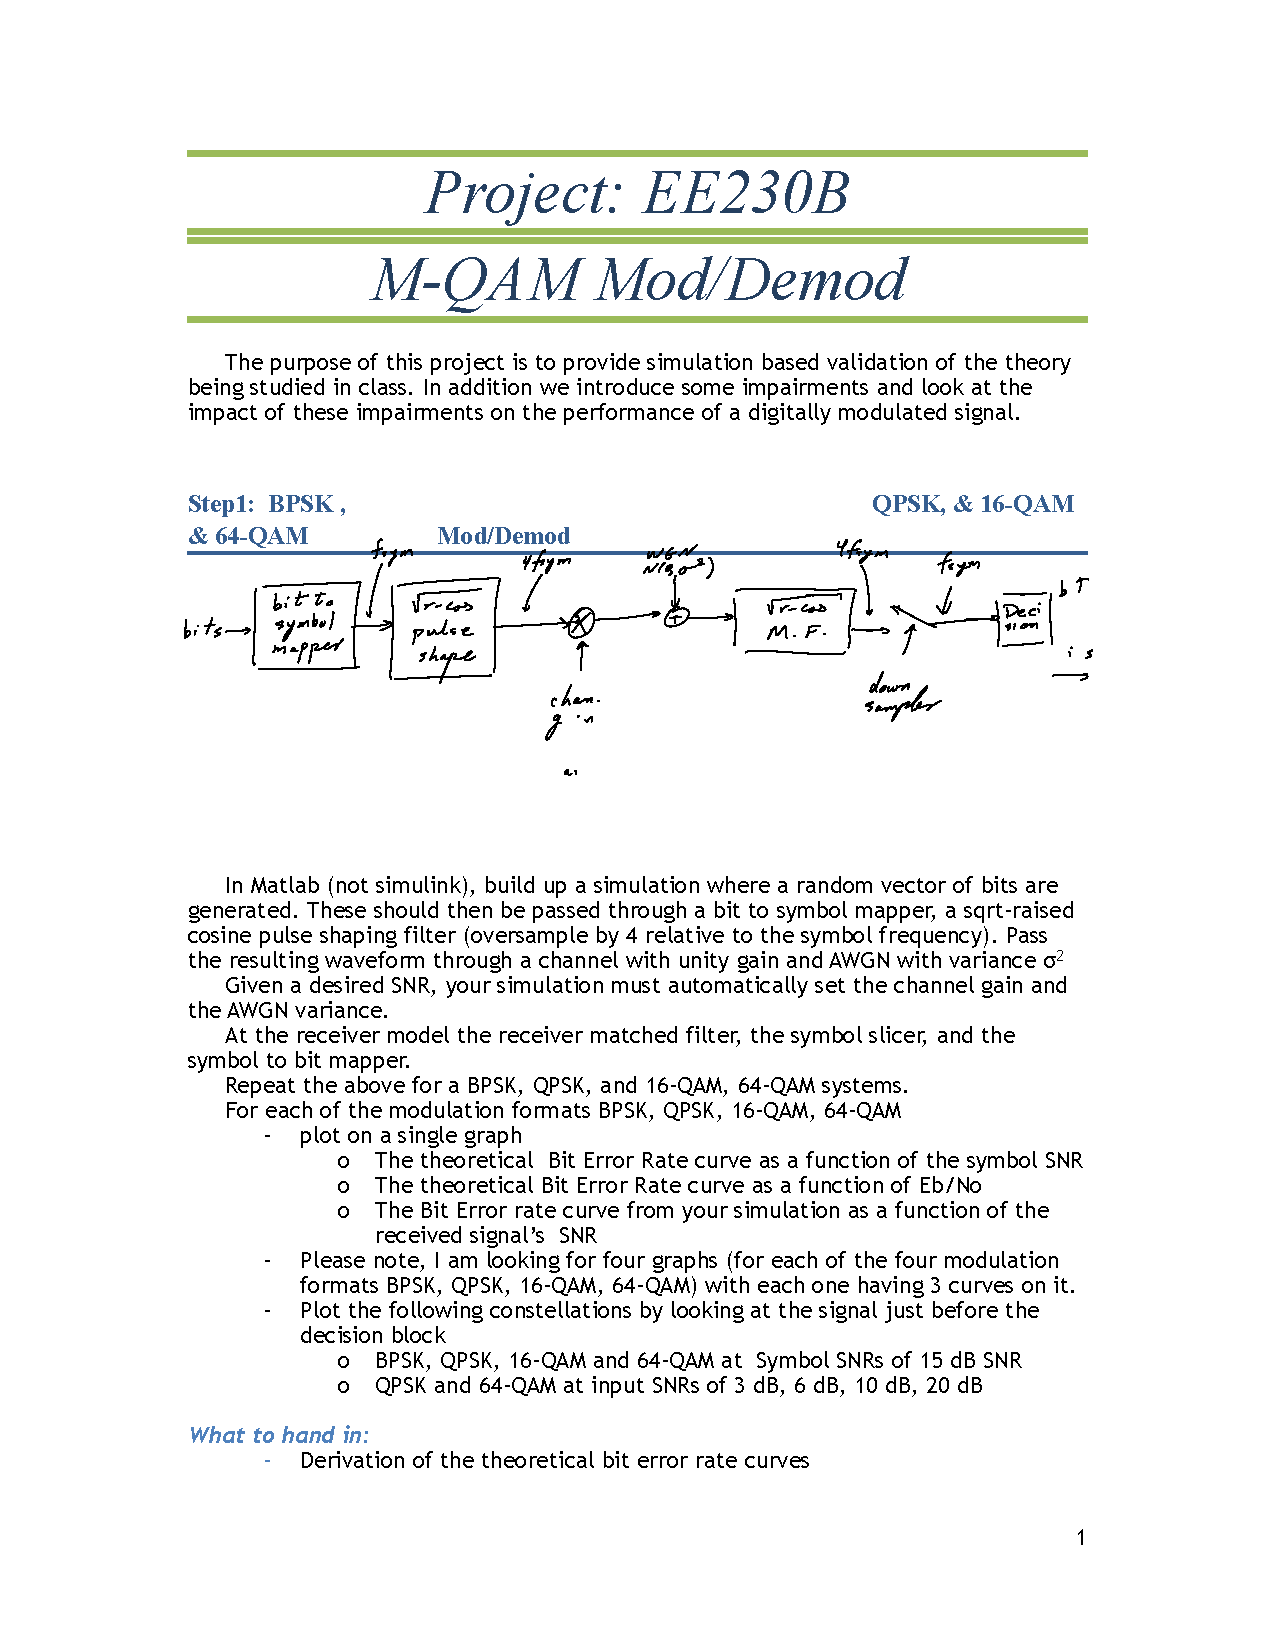
\includepdf[pages={1-5}]{project_overview.pdf}
\cleardoublepage
\newpage

\section{Communication Background}
\subsection{Feedback Theory}
\label{app:feedback}
In control theory when there is steady state error in the open loop system, feedback, or `closing the loop' can track out the error. This is appropriate for our simulation because we introduced frequency steady state error.  Depending on the order of the system, this error can become unbounded and damning.  Simple feedback can track this error if the open loop system Type is 0.  Recall, a system is of Type N when there are N poles at the s-plane origin.  Here however, we have a Type 1 system - ramp input of phase error.  The frequency offset introduced is actually a Type 1 phase error [Equation~\ref{eq:phaseToFreq}].  Introducing an additional integrator increases the order of the closed loop system to allow bounding of higher type systems. Notice in Figure~\ref{fig:system}, the loop filter is Proportional-Integral and the VCO is as well. With two integrators in the feedback path, we can bound phase error to a constant steady state level.  \\

\subsection{Data Conversion}
\label{app:converter}
Data conversion, the process of taking a continuous signal and descretizing it, can lead to additional and sometimes catastrophic errors.\\

Recall, digital signals are quantized into samples, discrete points in time.  Conversely, an analog signal has a continuous value.  Going from one to the other requires a converter.  To take an analog signal and digitize it, an Analog-to-Digial Converter (A/D) is used.  Both types of signals are shown in Figure~\ref{fig:digitization}.  There is a wrinkle: the rate of conversion is critical to preserving the information.  By the Nyquist-Shannon Sampling Theorem (\ref{eq:nyquist}), the sampling frequency must be at least twice the highest frequency in the signal.  Without reaching this frequency, the samples can wrongfully convey a lower frequency signal, alias, of the true signal.  This is shown in Figure~\ref{fig:alias}.  

\begin{align}
\label{eq:nyquist}
f_s \geq 2 f_{max}
\end{align}

\begin{figure}[h]
        \centering
        \begin{subfigure}[b]{0.4\textwidth}
                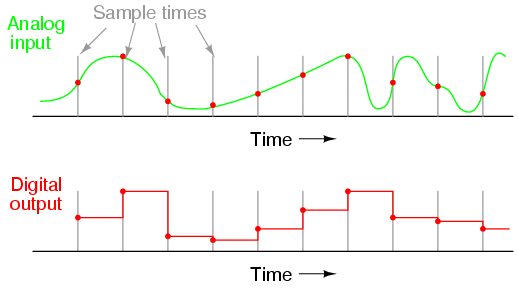
\includegraphics[width=\textwidth]{digitization.png}
                \caption{Analog and Digital signals}
                \label{fig:digitization}
        \end{subfigure}%
        \qquad \quad %add desired spacing between images, e. g.~, \quad, \qquad etc.
          %(or a blank line to force the subfigure onto a new line)
        \begin{subfigure}[b]{0.5\textwidth}
                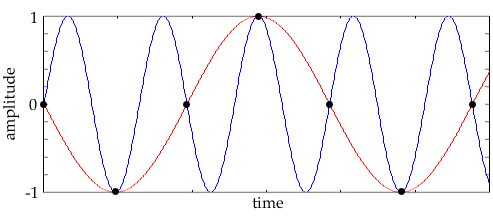
\includegraphics[width=\textwidth]{aliasing.jpg}
                \caption{Aliasing \label{fig:alias}}
                \label{fig:alias}
        \end{subfigure}
        \caption{Digital Conversion \label{fig:digitize}}
\end{figure}

\newpage
\subsection{Inter Symbol Interference and Equalization}
\label{app:ISIbackground}
Inter Symbol Interference (ISI) is when residual signal from symbols meddles the level of subsequent symbols.  Because of the bandlimiting, where the response of the system is zero above a limiting frequency, the symbols will interfere with one another. To deal with the dispersion, the Zero-ISI condition [\ref{thm:zero}] must be met.  A number of techniques can be utilized to accomplish what effectively amounts to canceling out delayed versions of symbols:

\begin{itemize}
\item Use $C^{-1}\left(f\right)$ to undo the channel
\item Use precoding
\item Use Nyquist's Pulse-Shaping Criterion and MLSE
\item Use an Equalizer
\end{itemize}

For this to be effective, the system channel medium must be known or estimated [Section~\ref{sec:estimate}].\\

\begin{thm}
\label{thm:zero}
Zero-ISI:
$$x\left(nT\right) = \left\{
\begin{array}{c c}
1 & \quad n=0 \\
0 & \quad \text{else}
\end{array} \right.$$
\end{thm}

\begin{figure}[b]
\centering
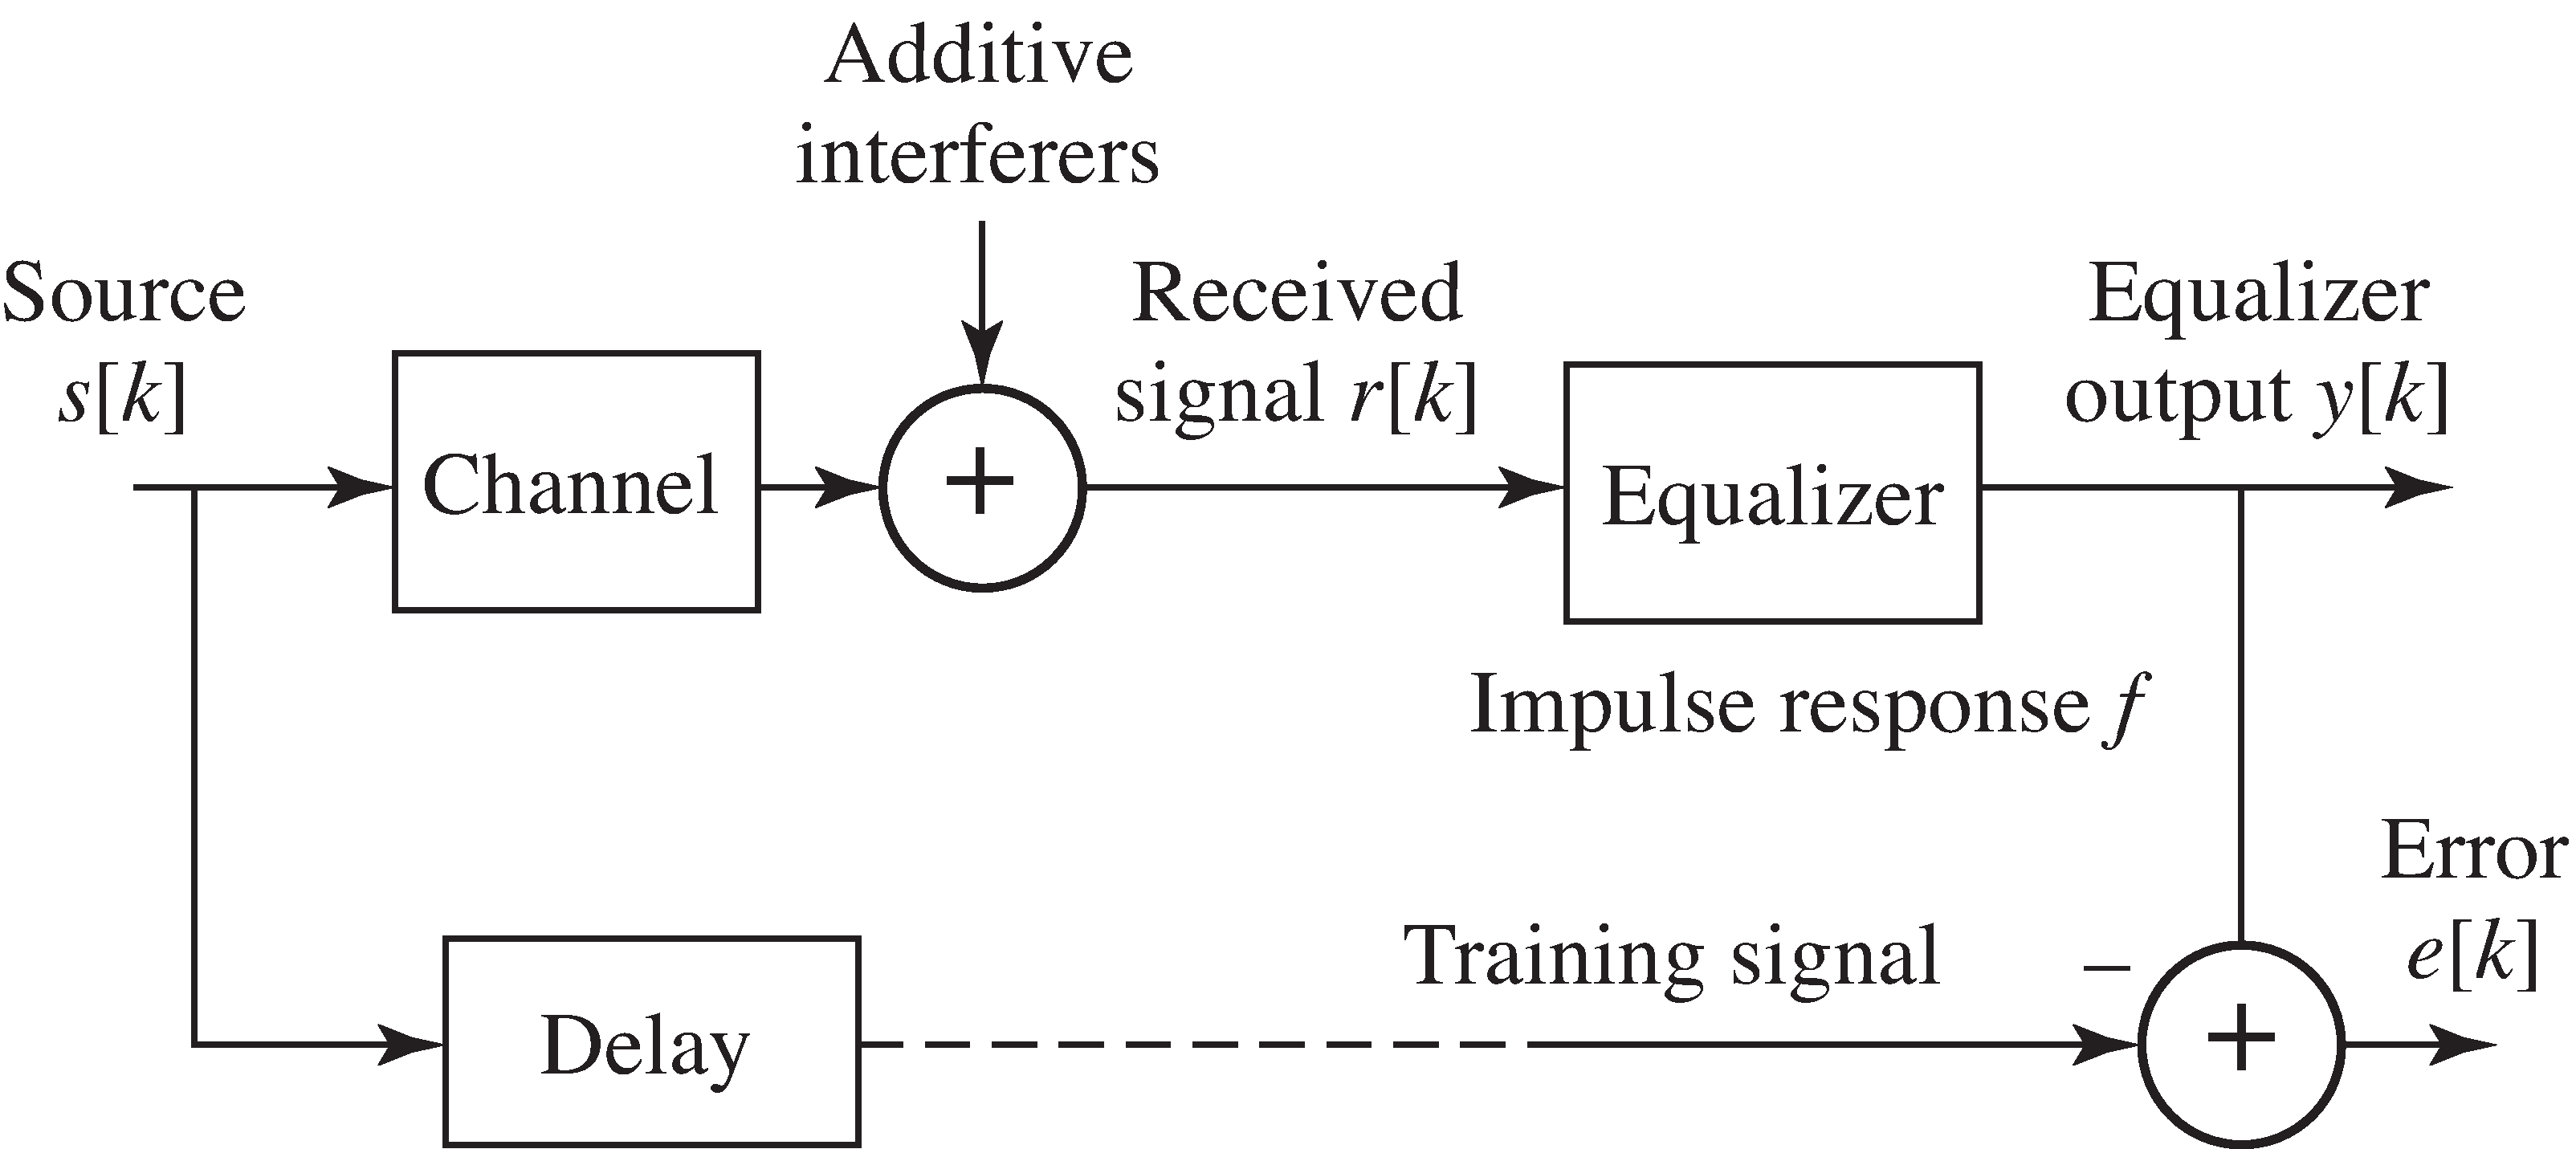
\includegraphics[width=.6\textwidth]{equalizer.png}
\caption{Generic Equalizer Filter to zero out the ISI\label{fig:equalizer}}
\end{figure}

\subsection{Estimation}
\label{app:estimate}
Considering this system, where Table~\ref{tab:filtersummary} describes the variables and Table~\ref{tab:Paramsummary} describes the dimension parameters, the channel is must be known before anything else. \\

To do channel estimation, a known sequence is sent through the system and error on the signal at output is measured.  That is, the input ($r$) and output ($y$) of the filter are known, and the tap weights ($f$) are to be determined - we can look at the impulse response of the unknown channel facing the known input.  Once the channel is understood, we can use an assortment of metrics to perform equalization.

\subsection{Equalization}
\label{app:equal}
An equalizer is a filter that zeros out the ISI in the end-to-end system.  It can be preset to handle the channel, or can adapt to the time-varying nature of a channel.  In the latter case, the equalizer parameter are adjusted on the fly by periodic transmission of a known sequence to re-estimate the channel.  In either case, the equalizer is a filter whose frequency response counteracts the system model such that Condition~\ref{thm:zero} is met. 

\begin{table}[H]
\begin{center}
\begin{tabular}{|c|c|c|c|}
\hline Variable & Meaning & Dimensions \\
\hline \hline
$\mathbf{I}$ & Symbol Source & $ m \times 1$ \\ \hline
$\mathbf{s}$ & Source & $m\times 1 $\\ \hline
$\mathbf{r}$ & Received Signal & $m\times 1$ \\ \hline
$R$ & Channel Response Matrix & $p\times n$ \\ \hline
$\mathbf{f}$ & Tap Line / Impulse Response & $n\times 1 $ \\ \hline
$\mathbf{y}$ & Equalizer Output & $ m\times 1 $ \\ \hline
 $\mathbf{e}$ & Training Error & $ m\times 1 $ \\ \hline
\end{tabular}
\caption{Summary of Signal Variables} \label{tab:filtersummary}
\end{center}
\end{table}

\begin{table}[b]
\begin{center}
\begin{tabular}{|c|c|}
\hline Parameter & Meaning \\
\hline \hline
$m$ & Signal Length \\ \hline
$N$ & Channel Filter Order \\ \hline
$n$ & Equalizer Filter Order \\ \hline
$p$ & Training Sequence Length \\ \hline
\end{tabular}
\caption{Summary of Parameters} \label{tab:Paramsummary}
\end{center}
\end{table}

The FIR form of the equalizer can then be written as Equation~\ref{eq:equalizerVector} and Equation~\ref{eq:equalizerMatrix}.  The compact form of this relation uses a matrix equation where the filter is expressed as a Toeplitz matrix.  This neat fact allows us to use the power of linear algebra to solve for the zero forcing channel.  
  
 
\begin{figure}[H]
\centering
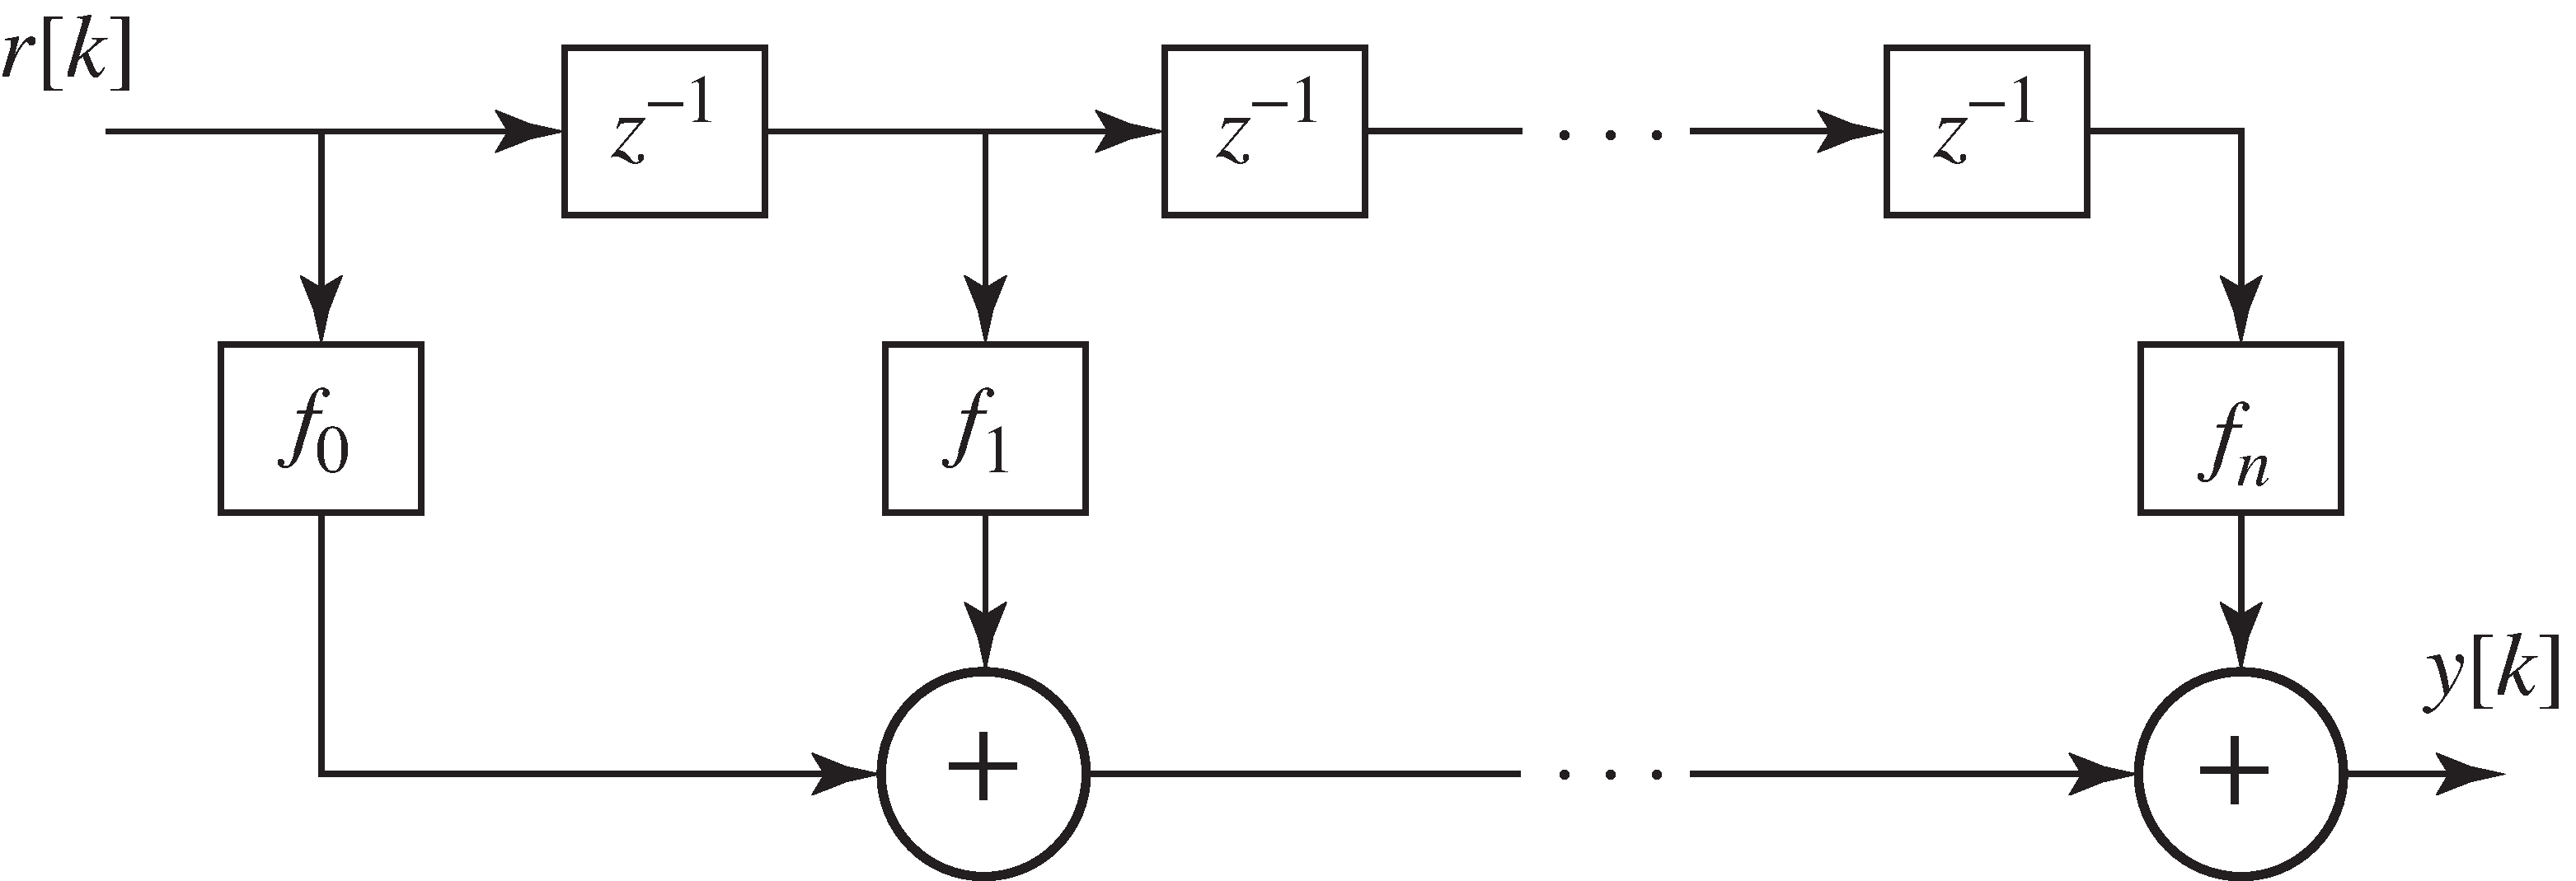
\includegraphics[width=.6\textwidth]{tapEqualizer.png}
\caption{Tapped Delay Line Represenation\label{fig:tap}}
\end{figure}

\begin{equation}
\label{eq:equalizer}
y\left[k\right] = \sum_{j=0}^n f_jr\left[k-j\right]
\end{equation}

The direct form of the FIR equalizor is shown in Figure~\ref{fig:tap}.  This is a subblock diagram view of the equalizer filter.  The transfer function can be gathered from Equation~\ref{eq:equalizer}.  The objective of this filter is to counter the system channel.  \\

\begin{equation}
\label{eq:equalizerVector}
\left[ \begin{array}{c}
 y \left[n+1\right] \\
 y \left[n+2\right] \\
 y \left[n+3\right] \\
\vdots  \\
y\left[ p \right] \end{array} \right] = 
\begin{bmatrix} 
r \left[ n+1\right]  & r[n] & \cdots & r\left[ 1 \right] \\ 
r \left[ n+2\right]  & r[n+1] & \cdots & r\left[ 2 \right] \\ 
r \left[ n+2\right]  & r[n+2] & \cdots & r\left[ 3 \right] \\ 
\vdots & \vdots & & \vdots \\
r \left[p \right] & r\left[ p-1 \right] & \cdots & r\left[ p-n \right]
\end{bmatrix}
 \left[ \begin{array}{c} f_0 \\ f_1 \\ f_2 \\ \vdots \\ f_n \end{array} \right]
\end{equation}

\begin{equation}
\label{eq:equalizerMatrix}
\mathbf{y} = R\mathbf{f}
\end{equation}
What we want is force the channel to zero for all other symbols other than the present one.  As an aside, because there is delay in the system, the intuitive sense of causality is blurred. That is, forward symbols from the present moment can actually cause interference to the present symbol. 

\newpage
\section{Random Bit Sequence Generator}
\label{app:random_bit_generator}
\lstinputlisting{random_bit_generator.m}

\section{Bit to Symbol Mapper}
\label{app:bittosym}

\subsection{QPSK Modulation}
\label{app:qpsk_mod}
\lstinputlisting{qpsk_mod.m}

\subsection{16-QAM Modulation}
\label{app:qam_16_mod}
\lstinputlisting{QAM_16_mod.m}

\section{Up Sampler}
\label{app:impulse_train}
\lstinputlisting{impulse_train.m}

\section{Square Root Raised Cosine Filter}
\label{app:sqrt_raised_cosine}
\lstinputlisting{sqrt_raised_cosine.m}

\section{Channel Models}
\subsection{Ideal Complex AWGN Channel}
\label{app:awgn_channel}
\lstinputlisting{awgn_complex_channel.m}

\subsection{Bandlimited Channel}
\label{app:bandlimited}
\lstinputlisting{bandlimited_channel.m}

\subsection{Frequency Offset}
\label{app:freq}
\lstinputlisting{freq_offset.m}

\section{Sampler}
\label{app:sampler}
\lstinputlisting{sampler.m}

\section{Decision Block}
\label{app:dblocks}
\subsection{QPSK Demodulation}
\label{app:qpsk_demod}
\lstinputlisting{qpsk_demod.m}

\subsection{16-QAM Demodulation}
\label{app:16qam_demod}
\lstinputlisting{QAM_16_demod.m}

\section{Equalizers}
\subsection{ZF Equalizer}
\label{app:zf}
\lstinputlisting{ZFEqualizer.m}


\section{Butterworth Filter}
\label{app:butterworth}
\lstinputlisting{ButterworthFilter.m}

\section{Conversion}
\label{app:convert}
\subsection{Zero Order Interpolation}
\label{app:da}
\lstinputlisting{ZeroHoldInterpolation.m}
\subsection{Zero Order Decimation}
\label{app:ad}
\lstinputlisting{ZeroHoldDecimation.m}

\section{Simulations Related Code Snippets}
\subsection{TX-End}
\label{app:TX_snip}
\lstinputlisting{TX_snippet.m}
\subsection{Channel}
\label{app:chan_snip}
\lstinputlisting{channel_snippet.m}
\subsection{RX-End}
\label{app:RX_snip}
\lstinputlisting{RX_snippet.m}
\end{document}
